\documentclass{style}

\answertrue

\exwheretrue


\begin{document}
	
\renewcommand{\labelenumi}{\arabic{enumi}.}
\renewcommand{\labelenumii}{(\arabic{enumii})}
\renewcommand{\labelenumiii}{\roman{enumiii}.}



%全国卷


\gaokaoheader{2020}{全国\lmd{1}卷}



\gaokaoxz




\begin{enumerate}
\item
行驶中的汽车如果发生剧烈碰撞,车内的安全气囊会被弹出并瞬间充满气体。若碰
撞后汽车的速度在很短时间内减小为零,关于安全气囊在此过程中的作用,下列说
法正确的是 \xzanswer{D} 


\fourchoices
{增加了司机单位面积的受力大小}
{减少了碰撞前后司机动量的变化量}
{将司机的动能全部转换成汽车的动能}
{延长了司机的受力时间并增大了司机的受力面积}


%题目类型:选择
%题目区域:动量:冲量
%题目难度:9
%思想方法:
%题目特征:材料分析
%题目备注:



\item 
火星的质量约为地球质量的$ 1/10 $,半径约为地球半径的$ 1/2 $,则同一物体在火星表
面与在地球表面受到的引力的比值约为 \xzanswer{B} 

\fourchoices
{0.2}
{0.4}
{2.0}
{2.5}

%题目类型:选择
%题目区域:万有引力
%题目难度:8
%思想方法:	
%题目特征:
%题目备注:

\item 
如图,一同学表演荡秋千,已知秋千的两根绳长均为$ 10 \ m $,该同学
和秋千踏板的总质量约为$ 50 \ kg $,绳的质量忽略不计,当该同学荡到
秋千支架的正下方时,速度大小为$ 8 \ m/s $,此时每根绳子平均承受的
拉力约为 \xzanswer{B} 
% TODO: \usepackage{graphicx} required
\begin{figure}[h!]
\centering
%\includegraphics[width=0.12\linewidth]{picture/screenshot034}
 \includesvg[width=0.16\linewidth]{picture/svg/GZ-3-tiyou-0608} 
\end{figure}



\fourchoices
{$ 200 \ N $}
{$ 400 \ N $}
{$ 600 \ N $}
{$ 800 \ N $}

%题目类型:选择
%题目区域:曲线运动:圆周
%题目难度:7
%思想方法:
%题目特征:材料分析
%题目备注:荡秋千的过程,轨迹为一圆。


\item 
图 \subref{2020-4-a} 所示的电路中,$ K $与$ L $间接一
智能电源,用以控制电容器$ C $两端的
电压$ U_{c} $,如果$ U_{c} $随时间$ t $的变化如图
\subref{2020-4-b} 所示,则下列描述电阻$ R $两端电
压$ U_{R} $随时间$ t $变化的图像中,正确的是 \xzanswer{A} 
\begin{figure}[h!]
\centering
\begin{subfigure}{0.4\linewidth}
\centering
\includesvg[width=0.5\linewidth]{picture/svg/GZ-3-tiyou-0615} 
\caption{}\label{2020-4-a}
\end{subfigure}
\hfil
\begin{subfigure}{0.4\linewidth}
\centering
\includesvg[width=0.7\linewidth]{picture/svg/GZ-3-tiyou-0616} 
\caption{}\label{2020-4-b}
\end{subfigure}
%\includesvg[width=0.83\linewidth]{picture/svg/GZ-3-tiyou-0592}
 %\includesvg[width=0.53\linewidth]{picture/svg/GZ-3-tiyou-0607}\\ 
 %\vspace{0.5em}
 %\includesvg[width=0.63\linewidth]{picture/svg/GZ-3-tiyou-0606} 
\end{figure}



\pfourchoices
{\includesvg[width=4.3cm]{picture/svg/GZ-3-tiyou-0611}}
{\includesvg[width=4.3cm]{picture/svg/GZ-3-tiyou-0612}}
{\includesvg[width=4.3cm]{picture/svg/GZ-3-tiyou-0613}}
{\includesvg[width=4.3cm]{picture/svg/GZ-3-tiyou-0614}}



%题目类型:选择
%题目区域:电路
%题目难度:6
%思想方法:
%题目特征:图像选择
%题目备注:利用排除法即可快速选出。


\item 
一匀强磁场的磁感应强度大小为$ B $,方向垂直于纸面向外,其边界如图中虚线所示,
$ \overarc{ab} $为半圆,$ ac $、$ bd $与直径$ ab $共线,$ ac $间的距离等于半圆的半径。一束质量为$ m $、
电荷量为$ q(q>0) $的粒子,在纸面内从$ c $点垂直于$ ac $射
入磁场,这些粒子具有各种速率,不计粒子之间的相互作用。在磁场中运动时间最长的粒子,其运动时间为 \xzanswer{C} 
\begin{figure}[h!]
\centering
\includesvg[width=0.3\linewidth]{picture/svg/GZ-3-tiyou-0596}
\end{figure}




\fourchoices
{$\frac{7 \pi m}{6 q B}$}
{$\frac{5 \pi m}{4 q B}$}
{$\frac{4 \pi m}{3 q B}$}
{$\frac{3 \pi n}{2 q B}$}


%题目类型:选择
%题目区域:磁场
%题目难度:4
%思想方法:
%题目特征:
%题目备注:过$ c $点作$ \overarc{ab} $的切线,交点处即为运动时间最长的点。

\item 
下列核反应方程中, \ce{X_1} 、 \ce{X_2} 、 \ce{X_3} 、 \ce{X_4} ,代表$ \alpha $粒子的有 \xzanswer{BD} 

\fourchoices
{ \ce{_{1}^{2}H + ^{2}_{1}H \rightarrow ^{1}_{0} n + X_{1} }}
{\ce{^{2}_{1}H + ^{3}_{1}H \rightarrow ^{1}_{0}n + X_{2} }}
{ \ce{^{235}_{92}H + ^{1}_{0}n \rightarrow ^{144}_{56}Ba + ^{89}_{36}Kr + 3X_{3} }}
{ \ce{ ^{1}_{0} n + \ce{^{6}_{3}Li} \rightarrow ^{3}_{1}H + X_{4} }}

%题目类型:选择
%题目区域:原子物理
%题目难度:8
%思想方法:
%题目特征:


\item 
一物块在高$ 3.0 \ m $、长$ 5.0 \ m $的斜面顶端从静止开始沿斜
面下滑,其重力势能和动能随下滑距离$ s $的变化如图中
直线 \lmd{1} 、 \lmd{2} 所示,重力加速度取$ 10 \ m/s^{2} $,则 \xzanswer{AB} 
\begin{figure}[h!]
\centering
\includesvg[width=0.3\linewidth]{picture/svg/GZ-3-tiyou-0594}
\end{figure}



\fourchoices
{物块下滑过程中机械能不守恒}
{物块与斜面间的动摩擦因数为$ 0.5 $}
{物块下滑时加速度的大小为$ 6.0 \ m/s^{2} $}
{当物块下滑$ 2.0 \ m $时机械能损失了$ 12 \ J $}


%题目类型:选择
%题目区域:能量守恒:动能定理
%题目难度:5
%思想方法:
%题目特征:图像分析
%题目备注:利用好斜率与截距,即可快速完成。


\item 
如图,$ U $形光滑金属框$ abcd $置于水平绝缘平台上,$ ab $和$ dc $边平行,和$ bc $边垂直。
$ ab $、$ dc $足够长,整个金属框电阻可忽略,一根具有一定电阻的导体棒$ MN $置于金属
框上,用水平恒力$ F $向右拉动金属框,运动过程中,装置始终处于竖直向下的匀强
磁场中,$ MN $与金属框保持良好接触,且与$ bc $边保持平行。经过一段时间后 \xzanswer{BC} 

\begin{figure}[h!]
\centering
\includesvg[width=0.33\linewidth]{picture/svg/GZ-3-tiyou-0597}
\end{figure}


\fourchoices
{金属框的速度大小趋于恒定值}
{金属框的加速度大小趋于恒定值}
{导体棒所受安培力的大小趋于恒定值}
{导体棒到金属框$ bc $边的距离趋于恒定值}

%题目类型:选择
%题目区域:磁场
%题目难度:3
%思想方法:极限:假设:隔离
%题目特征:
%题目备注:最终状态是速度之差恒定,对应两种情况:一是二者匀速,二是二者加速度相等。




\gaokaosy

\item 
某同学用伏安法测量一阻值为几十欧姆的电阻$ R_{x}$,所用电压
表的内阻为$ 1 \ K\Omega $,电流表内阻为$ 0.5 \ \Omega $,该同学采用两种测量方案,
一种是将电压表跨接在图 \subref{2020:全国1:9a} 所示电路的$ O $、$ P $两点之间,另一
种是跨接在$ O $、$ Q $两点之间,测量得到如图 \subref{2020:全国1:9b} 所示的两条$ U-I $图线,其中$ U $与$ I $分
别为电压表和电流表的示数。
\begin{figure}[!htp]
\centering
%\includesvg[width=0.3\linewidth]{picture/svg/GZ-3-tiyou-0598}
% \includesvg[width=0.3\linewidth]{picture/svg/GZ-3-tiyou-0609} 
\begin{subfigure}{0.25\linewidth}
\centering
\includesvg[width=1\linewidth]{picture/svg/GZ-3-tiyou-0617} 
\caption{}\label{2020:全国1:9a}
\end{subfigure}
\hfill
\begin{subfigure}{0.71\linewidth}
\centering
\includesvg[width=1\linewidth]{picture/svg/GZ-3-tiyou-0618} 
\caption{}\label{2020:全国1:9b}
\end{subfigure}
\end{figure}



回答下列问题$ : $

\begin{enumerate}
\item
图 \subref{2020:全国1:9b} 中标记为 \lmd{2} 的图线是采用电压表跨接在 \underlinegap (填“$ O $、$ P $”或“$ O $、$ Q $”)两点的方案测量得到的。





\item \label{2020-9-2}
根据所用实验器材和图 \subref{2020:全国1:9b} 可判断,由图线 \underlinegap (填“\lmd{1}”或“\lmd{2}”)得到
的结果更接近待测电阻的真实值,结果为 \underlinegap $ \Omega $
(保留1位小数)。



\item 
考虑到实验中电表内阻的影响,需对$ (2) $中得到的结果进行修正,修正后待
测电阻的阻值为 \underlinegap 
$ \Omega $(保留1位小数)。

\end{enumerate}


\tk{
\begin{enumerate}
\item
$ O $、$ P $	
\item 
\lmd{1} \quad $ 50.5 $
\item 
$ 50.0 $
\end{enumerate}
} 

%题目类型:实验
%题目区域:电路
%题目难度:7
%思想方法:
%题目特征:
%题目备注:电压表内接或者外接需要计算其临界电阻:$ R_{0}=\sqrt{R_{A} R_{V} } $当$ R>R_{0} $时采用内接;当$ R<R_{0} $时采用外接。



\item 
某同学用如图所示的实验装置验
证动量定理,所用器材包括,气垫导
轨、滑块(上方安装有宽度为$ d $的遮
光片)、两个与计算机相连接的光电
门、砝码盘和砝码等。

\begin{figure}[h!]
\centering
\includesvg[width=0.46\linewidth]{picture/svg/GZ-3-tiyou-0601}
\end{figure}


实验步骤如下:

\begin{enumerate}
\item
开动气泵,调节气垫导轨,轻推滑块,当滑块上的遮光片经过两个光电门的遮
光时间 \underlinegap 时,可认为气垫导轨水平;

\item 
用天平测砝码与砝码盘的总质量$ m_{1} $、滑块(含遮光片)的质量$ m_2 $;
\item 
用细线跨过轻质定滑轮将滑块与砝码盘连接,并让细线水平拉动滑块:
\item 
令滑块在砝码和砝码盘的拉动下从左边开始运动,和计算机连接的光电门能测
量出遮光片经过$ A $、$ B $两处的光电门的遮光时间$ \Delta t_{1} $、$ \Delta t_2 $及遮光片从$ A $运动到$ B $所用
的时间$ t_{ 12 } $;


\item 
在遮光片随滑块从$ A $运动到$ B $的过程中,如果将砝码和砝码盘所受重力视为
滑块所受拉力,拉力冲量的大小$ I= $ \underlinegap 
,滑块动量改变量的大小$ \Delta p= $ \underlinegap ; 
(用
题中给出的物理量及重力加速度$ g $表示)

\item 
某次测量得到的一组数据为:$ d=1.000 \ cm , m_{1}=1.50 \times 10^{-2} \ kg, m_{2} =0.400 \ kg $,
$ \Delta t_{1}=3.900 \times 10^{-2} \ s , \Delta t_2=1.270 \times 10^{-2} \ s, t_{ 12}=1.50 \ s $,
取$ g=9.80 \ m/s^{2} $,计算可得
$ I = $ \underlinegap $ N \cdot s $,$ \Delta p = $ \underlinegap $ kg \cdot m \cdot s^{-1} $;
(结果均保留$ 3 $位有效数字)

\item 
定义$ \delta=\left|\frac{I-\Delta p}{I}\right| \times 100 \% $, 本次实验$ \delta= $ \underlinegap 
$ \% $(保留$ 1 $位有效数字)。

\end{enumerate}

\tk{
\begin{enumerate}
\item[(1)]
大约相等	
\item [(5)]
$m_{1} g t_{12}$ \quad 	$m_{2}\left(\frac{d}{\Delta t_{2}}-\frac{d}{\Delta t_{1}}\right)$
\item [(6)]
$ 0.221 $ \quad $ 0.212 $
\item [(7)]
$ 4 $	
\end{enumerate}
} 

%题目类型:实验
%题目区域:动量
%题目难度:7
%思想方法:
%题目特征:计算练习
%题目备注:




\newpage

\gaokaojs


\item 
我国自主研制了运---20 重型运输机,飞机获得的升力大小$ F $可用$ F=kv^{2} $描写,$ k $为
系数; $ v $是飞机在平直跑道上的滑行速度,$ F $与飞机所受重力相等时的$ v $称为飞机的起
飞离地速度,已知飞机质量为$ 1.21 \times 10^{5} \ kg $时,起飞离地速度为$ 66 \ m/s $;装载货物后质
量为$ 1.69 \times 10^{5} \ kg $,装载货物前后起飞离地时的$ k $值可视为不变。

\begin{enumerate}
\item
求飞机装载货物后的起飞离地速度;
\item 
若该飞机装载货物后,从静止开始匀加速滑行$ 1521 \ m $起飞离地,求飞机在滑行
过程中加速度的大小和所用的时间。





\end{enumerate}


\banswer{
\begin{enumerate}
\item
$v_{2}=78 \ m/s $
\item 
$a=2 \ m/s^{2} , t=39 \ s $
\end{enumerate}	
}

%题目类型:计算
%题目区域:直线运动
%题目难度:7
%思想方法:比例
%题目特征:
%题目备注:采用比例求解,简洁快速。


\item 
在一柱形区域内有匀强电场,柱的横截面是以$ O $为圆心,
半径为$ R $的圆,$ AB $为圆的直径,如图所示,质量为$ m $,电荷量
为$ q(q>0) $的带电粒子在纸面内自$ A $点先后以不同的速度进
入电场,速度方向与电场的方向垂直。已知刚进入电场时速度为
零的粒子,自圆周上的$ C $点以速率$ v_{0} $穿出电场,$ AC $与$ AB $的夹
角$ \theta=60 ^{ \circ } $,运动中粒子仅受电场力作用。
\begin{enumerate}
\item
求电场强度的大小;
\item 
为使粒子穿过电场后的动能增量最大,该粒子进入电场时的速度应为多大?
\item 
为使粒子穿过电场前后动量变化量的大小为$ mv_{0} $,该粒子进入电场时的速度应
为多大?




\end{enumerate}
\begin{figure}[h!]
\flushright
\includesvg[width=0.23\linewidth]{picture/svg/GZ-3-tiyou-0602}
\end{figure}






\banswer{
\begin{enumerate}
\item
$E=\frac{m v_{0}^{2}}{2 q R}$
\item 
$v_{1}=\frac{\sqrt{2} v_{0}}{4}$
\item 
$ 0 $或 $v_{2}=\frac{\sqrt{3} v_{0}}{2}$
\end{enumerate}
}

%题目类型:计算
%题目区域:电场
%题目难度:4
%思想方法:	
%题目特征:
%题目备注:

\newpage
\gaokaoxx{$ 3 - 3 $}



\item 
%选修 $ 3 - 3 $
\begin{enumerate}
\item
分子间作用力$ F $与分子间距$ r $的关系如图
所示,$ r=r_{1} $时,$ F=0 $,分子间势能由$ r $决定,规定两分子
相距无穷远时分子间的势能为零。若一分子固定于原点$ O $,
另一分子从距$ O $点很远处向$ O $点运动,在两分子间距减小
到$ r_{2} $的过程中,势能 \underlinegap (填“减小”“不变”或“增大”);
在间距由$ r_{2} $减小到$ r_{1} $的过程中,势能 \hfullline (填“减小”“不变”或“增大”);\\
在间距
等于$ r_{1} $处,势能 \underlinegap (填“大于”“等于”或“小于”)零。

\begin{figure}[h!]
\centering
\includesvg[width=0.23\linewidth]{picture/svg/GZ-3-tiyou-0603}
\end{figure}

\tk{减小、减小、小于}

%题目类型:填空
%题目区域:分子动理论
%题目难度:7
%思想方法:
%题目特征:图像分析
%题目备注:


\item 
甲、乙两个储气罐储存有同种气体(可视为理想气体)。甲罐的容积为
$ V $,罐中气体的压强为$ p$;乙罐的容积为$ 2 V $,罐中气体的压强为$ \frac{ 1 }{ 2 } p $。现通过连接两罐
的细管把甲罐中的部分气体调配到乙罐中去,罐中气体温度相同且在调配过程中保持
不变,调配后两罐中气体的压强相等。求调配后:
\begin{enumerate}
\item
两罐中气体的压强;
\item 
甲罐中气体的质量与甲罐中原有气体的质量之比。
\end{enumerate}




\banswer{
\begin{enumerate}
\item
$ \frac{ 2 }{ 3 } p $
\item 
$ \frac{ 2 }{ 3 } $
\end{enumerate}
}


%题目类型:计算
%题目区域:热学:理想气体状态方程
%题目难度:6
%思想方法:
%题目特征:
%题目备注:


\end{enumerate}







\newpage
\gaokaoxx{$ 3 - 4 $}


\item 
%选修 $ 3 - 4 $
\begin{enumerate}
\item
在下列现象中,可以用多普勒效应解释的有 \underlinegap 。
(填正确答案标号,
选对1个得2分,选对2个得4分,选对3个得5分每选错1个扣3分,最低得分为
0分)
\fivechoices
{雷雨天看到闪电后,稍过一会儿才能听到雷声}
{超声波被血管中的血流反射后,探测器接收到的超声波频率发生变化}
{观察者听到远去的列车发出的汽笛声,音调会变低}
{同一声源发出的声波,在空气和水中传播的速度不同}
{天文学上观察到双星(相距较近、均绕它们连线上某点做圆周运动的两颗恒星)光谱随时间的周期性变化}

\tk{BCE} 

%题目类型:选择
%题目区域:机械波:多普勒效应
%题目难度:
%思想方法:
%题目特征:
%题目备注:


\item 
一振动片以频率$ f $做简谐振动时,固定在振动片
上的两根细杆同步周期性地触动水面上$ a $、$ b $两点,两波源发出的
波在水面上形成稳定的干涉图样、$ c $是水面上的一点,$ a $、$ b $、$ c $间
的距离均为$ l $,如图所示。已知除$ c $点外,在$ ac $连线上还有其他振
幅极大的点,其中距$ c $最近的点到$ c $的距离为$ \frac{ 3 }{ 8 } l $,求:
\begin{enumerate}
\item
波的波长;

\item 
波的传播速度。

\end{enumerate}
\begin{figure}[h!]
\flushright
\includesvg[width=0.2\linewidth]{picture/svg/GZ-3-tiyou-0604}
\end{figure}

\banswer{
\begin{enumerate}
\item
$\frac{1}{4} l$
\item 
$\frac{1}{4} f l$
\end{enumerate}
}


%题目类型:计算
%题目区域:机械波:干涉
%题目难度:
%思想方法:	
%题目特征:
%题目备注:


\end{enumerate}




\end{enumerate}



%
\gaokaoheader{2020}{全国\lmd{2}卷}



\gaokaoxz


\begin{enumerate}
\item
管道高频焊机可以对由钢板卷成的圆管的接缝实施焊接。焊机的原理如图所示,圆管通过一个接有高
频交流电源的线圈,线圈所产生的交变磁场使圆管中产生交变电流,电流产生的热量使接缝处的材料
熔化将其焊接。焊接过程中所利用的电磁学规律的发现者为 \xzanswer{D} 
\begin{figure}[h!]
\centering
\includesvg[width=0.33\linewidth]{picture/svg/GZ-3-tiyou-0619}
\end{figure}


\fourchoices
{库仑}
{霍尔}
{洛伦兹}
{法拉第}




\item
若一均匀球形星体的密度为$ \rho $,引力常量为 $ G $,则在该星体表面附近沿圆轨道绕其运动的卫星的周期是 \xzanswer{A} 

\fourchoices
{$\sqrt{\frac{3 \pi}{G \rho}}$}
{$ \sqrt{\frac{4 \pi}{G \rho}}$}
{$ \sqrt{\frac{1}{3 \pi G \rho}}$}
{$\sqrt{\frac{1}{4 \pi G \rho}}$}



\item
如图,在摩托车越野赛途中的水平路段前方有一个坑,该坑沿摩托车前进方向的水平宽度为 $ 3h $,其左
边缘 $ a $ 点比右边缘 $ b $ 点高 $ 0.5h $。若摩托车经过 $ a $ 点时的动能为 $ E_{1} $,它会落到坑内 $ c $ 点。$ c $ 与 $ a $ 的水平距
离和高度差均为 $ h $;若经过 $ a $ 点时的动能为 $ E_{2} $,该摩托车恰能越过坑到达 $ b $ 点。
$\frac{E_{2}}{E_{1}}$
等于 \xzanswer{B} 
\begin{figure}[h!]
\centering
\includesvg[width=0.43\linewidth]{picture/svg/GZ-3-tiyou-0620}
\end{figure}


\fourchoices
{$ 20 $}
{$ 18 $}
{$ 9.0 $}
{$ 3.0 $}




\item
$ CT $ 扫描是计算机 $ X $ 射线断层扫描技术的简称,$ CT $ 扫描机可用于对多种病情的探测。图 \subref{2020:全国2:4a} 是某种 $ C $
$ T $ 机主要部分的剖面图,其中 $ X $ 射线产生部分的示意图如图 \subref{2020:全国2:4b} 所示。图 \subref{2020:全国2:4b} 中 $ M $、$ N $ 之间有一电
子束的加速电场,虚线框内有匀强偏转磁场;经调节后电子束从静止开始沿带箭头的实线所示的方向
前进,打到靶上,产生 $ X $ 射线(如图中带箭头的虚线所示);将电子束打到靶上的点记为 $ P $ 点。则 \xzanswer{D} 
\begin{figure}[h!]
\centering
\begin{subfigure}{0.45\linewidth}
\centering
\includesvg[width=0.9\linewidth]{picture/svg/GZ-3-tiyou-0621} 
\caption{}\label{2020:全国2:4a}
\end{subfigure}
\hfil
\begin{subfigure}{0.45\linewidth}
\centering
\includesvg[width=0.9\linewidth]{picture/svg/GZ-3-tiyou-0622} 
\caption{}\label{2020:全国2:4b}
\end{subfigure}

\end{figure}


\fourchoices
{$ M $ 处的电势高于 $ N $ 处的电势}
{增大 $ M $、$ N $ 之间的加速电压可使 $ P $ 点左移}
{偏转磁场的方向垂直于纸面向外}
{增大偏转磁场磁感应强度的大小可使 $ P $ 点左移}



\item
氘核 \ce{^{2}_{1}H} 可通过一系列聚变反应释放能量,其总效果可用反应式
\[ \ce{6^{2}_{1}H \rightarrow {2}_{4}^{2}He + 2^{1}_{0}n + 43.15MeV} \]
表示。海水中富含氘,已知 $ 1 \ kg $ 海水中含有的氘核约为 $ 1.0 \times 10^{22} $ 个,若全都发生聚变反应,其释放的能
量与质量为 $ M $ 的标准煤燃烧时释放的热量相等;已知 $ 1 \ kg $ 标准煤燃烧释放的热量约为 $ 2.9 \times 10^{7} \ J $,$ 1 \ MeV=1.6 \times 10^{-13} \ J $,则 $ M $ 约为 \xzanswer{C} 

\fourchoices
{$ 40 \ kg $}
{$ 100 \ kg $}
{$ 400 \ kg $}
{$ 1000 \ kg $}


\item
特高压输电可使输送中的电能损耗和电压损失大幅降低。我国已成功掌握并实际应用了特高压输电技术。假设从$ A $处采用$ 550 \ kV $的超高压向$ B $处输电,输电线上损耗的电功率为$ \Delta P $,到达$ B $处时电压下降了
$ \Delta U $。在保持$ A $处输送的电功率和输电线电阻都不变的条件下,改用$ 1100 \ kV $特高压输电,输电线上损耗
的电功率变为$ \Delta P ^{\prime} $,到达$ B $处时电压下降了$ \Delta U ^{\prime} $。不考虑其他因素的影响,则 \xzanswer{AD} 

\fourchoices
{$\Delta P^{\prime}=\frac{1}{4} \Delta P$}
{$\Delta P^{\prime}=\frac{1}{2} \Delta P$}
{$\Delta U^{\prime}=\frac{1}{4} \Delta U$}
{$\Delta U^{\prime}=\frac{1}{2} \Delta U$}



\item
如图,竖直面内一绝缘细圆环的上、下半圆分别均匀分布着等量异种电荷。$ a $、$ b $为圆环水平直径上的
两个点,$ c $、$ d $为竖直直径上的两个点,它们与圆心的距离均相等。则 \xzanswer{ABC} 
\begin{figure}[h!]
\centering
\includesvg[width=0.23\linewidth]{picture/svg/GZ-3-tiyou-0623}
\end{figure}


\fourchoices
{$ a $、$ b $两点的场强相等}
{$ a $、$ b $两点的电势相等}
{$ c $、$ d $两点的场强相等}
{$ c $、$ d $两点的电势相等}


\item
水平冰面上有一固定的竖直挡板,一滑冰运动员面对挡板静止在冰面上,他把一质量为$ 4.0 \ kg $的静止物
块以大小为$ 5.0 \ m/s $的速度沿与挡板垂直的方向推向挡板,运动员获得退行速度;物块与挡板弹性碰撞,
速度反向,追上运动员时,运动员又把物块推向挡板,使其再一次以大小为$ 5.0 \ m/s $的速度与挡板弹性
碰撞。总共经过$ 8 $次这样推物块后,运动员退行速度的大小大于$ 5.0 \ m/s $,反弹的物块不能再追上运动员。
不计冰面的摩擦力,该运动员的质量可能为 \xzanswer{BC} 

\fourchoices
{$ 48 \ kg $}
{$ 53 \ kg $}
{$ 58 \ kg $}
{$ 63 \ kg $}



\gaokaosy


\item 
一细绳跨过悬挂的定滑轮,两端分别系有小球 $ A $ 和 $ B $,如图所示。一实验小组用此装置测量小球 $ B $ 运
动的加速度。
\begin{figure}[h!]
\centering
\includesvg[width=0.14\linewidth]{picture/svg/GZ-3-tiyou-0624}
\end{figure}

令两小球静止,细绳拉紧,然后释放小球,测得小球 $ B $ 释放时的高度 $ h_{0} =0.590 \ m $,下降一段距离后的
高度 $ h=0.100 \ m $;由 $ h_{0} $ 下降至 $ h $ 所用的时间 $ T=0.730 \ s $。由此求得小球 $ B $ 加速度的大小为 $ a=$ \underlinegap $m/s^{2} $(保
留 $ 3 $ 位有效数字)。

从实验室提供的数据得知,小球 $ A $、$ B $ 的质量分别为 $ 100.0 \ g $ 和 $ 150.0 \ g $,当地重力加速度大小为 $ g=9.80 \ m/s^{2} $。根据牛顿第二定律计算可得小球 $ B $ 加速度的大小为 $ a ^{\prime}= $ \underlinegap $m/s^{2} $(保留 $ 3 $ 位有效数字)。

可以看出,$ a ^{\prime} $与 $ a $ 有明显差异,除实验中的偶然误差外,写出一条可能产生这一结果的原因: \hfullline 

\hfullline 。

\tk{1.84 \quad 1.96 \quad 滑轮的轴不光滑(或滑轮有质量)} 



\newpage
\item
某同学要研究一小灯泡 $ L $($ 3.6 \ V $,$ 0.30 \ A $)的伏安特性。所用器材有:电流表 $ A_{1} $(量程 $ 200 \ mA $,内
阻 $ R_{g1} =10.0 \ \Omega $),电流表 $ A_{2} $(量程 $ 500 \ mA $,内阻 $ R_{g2} =1.0 \ \Omega $)、定值电阻 $ R_{0} $(阻值 $ R_{0} =10.0 \ \Omega $)、滑动变
阻器 $ R_{1} $(最大阻值 $ 10 \ \Omega $)、电源 $ E $(电动势 $ 4.5 \ V $,内阻很小)、开关 $ S $ 和若干导线。该同学设计的电路
如图 \subref{2020:全国2:10a} 所示。


\begin{enumerate}
\item
根据图 \subref{2020:全国2:10a} ,在图 \subref{2020:全国2:10b} 的实物图中画出连线。
\begin{figure}[h!]
\centering
\begin{subfigure}{0.4\linewidth}
\centering
\includesvg[width=0.8\linewidth]{picture/svg/GZ-3-tiyou-0625} 
\caption{}\label{2020:全国2:10a}
\end{subfigure}
\hfil
\begin{subfigure}{0.4\linewidth}
\centering
\includesvg[width=0.8\linewidth]{picture/svg/GZ-3-tiyou-0626} 
\caption{}\label{2020:全国2:10b}
\end{subfigure}
\end{figure}

\item 
若 $ I_{1} $、$ I_{2} $ 分别为流过电流表 $ A_{1} $ 和 $ A_{2} $ 的电流,利用 $ I_{1} $、$ I_{2} $、$ R_{g1} $ 和 $ R_{0} $ 写出:小灯泡两端的电压 $ U= $ \underlinegap 
,流过小灯泡的电流 $ I= $ \underlinegap 。为保证小灯泡的安全,$ I_{1} $ 不能超过 \underlinegap $ mA $。

\item 
实验时,调节滑动变阻器,使开关闭合后两电流表的示数为零。逐次改变滑动变阻器滑片位置并
读取相应的 $ I_{1} $ 和 $ I_{2} $。所得实验数据在下表中给出。
\begin{table}[h!]
\centering 
\begin{tabular}{|l|l|l|l|l|l|l|}
\hline$I_{1} / \mathrm{mA}$ & 32 & 55 & 85 & 125 & 144 & 173 \\
\hline$I_{2} / \mathrm{mA}$ & 171 & 229 & 299 & 379 & 424 & 470 \\
\hline
\end{tabular}
\end{table} 





根据实验数据可算得,当 $ I_{1} =173 \ mA $ 时,灯丝电阻 $ R=$ \underlinegap $ \Omega $(保留 $ 1 $ 位小数)。


\item 
如果用另一个电阻替代定值电阻 $ R_{0} $,其他不变,为了能够测量完整的伏安特性曲线,所用电阻的
阻值不能小于 \underlinegap $ \Omega $(保留 $ 1 $ 位小数)。

\end{enumerate}

\tk{
\begin{enumerate}
\item
如图所示:
\begin{center}
\includesvg[width=0.53\linewidth]{picture/svg/GZ-3-tiyou-0627} 
\end{center}	
\item 	
$I_{1}\left(R_{g1}+R_{0}\right) \quad I_{2}-I_{1} \quad 180$
\item 
$ 11.6 $
\item 
$ 8.0 $
\end{enumerate}
} 



\newpage

\gaokaojs

\item
如图,在 $ 0 \leq x \leq h $, $ - \infty <y<+ \infty$ 区域中存在方向垂直于纸面的匀强磁场,磁感应强度 $ B $ 的大小可调,方
向不变。一质量为 $ m $,电荷量为 $ q $($ q>0 $)的粒子以速度 $ v_{0} $ 从磁场区域左侧沿 $ x $ 轴进入磁场,不计重力。
\begin{enumerate}
\item
若粒子经磁场偏转后穿过 $ y $ 轴正半轴离开磁场,分析说明磁场的方向,并求在这种情况下磁感应
强度的最小值 $ B_{m} $;
\item 
如果磁感应强度大小为
$\frac{B_{m}}{2}$,粒子将通过虚线所示边界上的一点离开磁场。求粒子在该点的运动
方向与 $ x $ 轴正方向的夹角及该点到 $ x $ 轴的距离。

\end{enumerate}
\begin{figure}[h!]
\flushright
\includesvg[width=0.27\linewidth]{picture/svg/GZ-3-tiyou-0628}
\end{figure}

\banswer{
\begin{enumerate}
\item
$B_{\mathrm{m}}=\frac{m v_{0}}{q h}$	
\item 	
粒子会穿过图中 $P$ 点离开磁场, 运动轨迹如图所示。
\begin{center}
\includesvg[width=0.43\linewidth]{picture/svg/GZ-3-tiyou-0629} 
\end{center}
设粒子在 $P$ 点的运动方向与 $x$ 轴正方向的夹角为 $\alpha$,易得$\alpha=\frac{\pi}{6}$。	\\
$P$ 点与 $x$ 轴的距离为$y=(2-\sqrt{3}) h$。
\end{enumerate}
}




\newpage
\item
如图,一竖直圆管质量为 $ M $,下端距水平地面的高度为 $ H $,顶端塞有一质量为 $ m $ 的小球。圆管由
静止自由下落,与地面发生多次弹性碰撞,且每次碰撞时间均极短;在运动过程中,管始终保持竖直。
已知 $ M=4m $,球和管之间的滑动摩擦力大小为 $ 4mg,g $ 为重力加速度的大小,不计空气阻力。
\begin{enumerate}
\item
求管第一次与地面碰撞后的瞬间,管和球各自的加速度大小;
\item 
管第一次落地弹起后,在上升过程中球没有从管中滑出,求管上升的最大高度;
\item 
管第二次落地弹起的上升过程中,球仍没有从管中滑出,求圆管长度应满足的条件。

\end{enumerate}
\begin{figure}[h!]
\flushright
\includesvg[width=0.2\linewidth]{picture/svg/GZ-3-tiyou-0630}
\end{figure}

\banswer{
\begin{enumerate}
\item
设此时管的加速度大小为$ a_{1} $,方向向下;球的加速度大小为$ a_{2} $,方向向上;$a_{1}=2 g, \quad a_{2}=3 g$。		
\item 
$H_{max}=\frac{13}{25} H$		
\item 
$L \geq \frac{152}{125} H$		
\end{enumerate}
}



\newpage

\gaokaoxx{$ 3 - 3 $}


\item
\begin{enumerate}
\item
下列关于能量转换过程的叙述,违背热力学第一定律的有 \underlinegap ,不违背热力学第一定
律、但违背热力学第二定律的有 \underlinegap 。(填正确答案标号)

\fourchoices
{汽车通过燃烧汽油获得动力并向空气中散热}
{冷水倒入保温杯后,冷水和杯子的温度都变得更低}
{某新型热机工作时将从高温热源吸收的热量全部转化为功,而不产生其他影响}
{冰箱的制冷机工作时从箱内低温环境中提取热量散发到温度较高的室内}

\tk{B \quad C} 



\item 
潜水钟是一种水下救生设备,它是一个底部开口、上部封闭的容器,外形与钟相似。潜
水钟在水下时其内部上方空间里存有空气,以满足潜水员水下避险的需要。为计算方便,将潜水钟简化为
截面积为 $ S $、高度为 $ h $、开口向下的圆筒;工作母船将潜水钟由水面上方开口向下吊放至深度为 $ H $ 的水下,
如图所示。已知水的密度为$ \rho $,重力加速度大小为 $ g $,大气压强为 $ p_{0} $,$H \gg h$,忽略温度的变化和水密度随深度的变化。
\begin{enumerate}
\item
求进入圆筒内水的高度 $ l $;
\item 
保持 $ H $ 不变,压入空气使筒内的水全部排出,求压入的空气在其压强为 $ p_{0} $ 时的体积。
\end{enumerate}
\begin{figure}[h!]
\flushright
\includesvg[width=0.25\linewidth]{picture/svg/GZ-3-tiyou-0631}
\end{figure}

\banswer{
\begin{enumerate}
\item
考虑到$ H \gg h>l $,将$ l^{2} $当作二阶小量略去,解得$l=\frac{\rho g H}{p_{0}+\rho g (H+h)} h$,正式答案为$l=\frac{\rho g H}{p_{0}+\rho g H} h$。
\item 	
解得$V=\left( 1+\frac{\rho g h}{p_{0}} \right) S H$,正式答案为$V=\frac{\rho g S H h}{p_{0}}$
\end{enumerate}
}






\end{enumerate}





\newpage

\gaokaoxx{$ 3 - 4 $}


\item 
\begin{enumerate}
\item
用一个摆长为 $ 80.0 \ cm $ 的单摆做实验,要求摆动的最大角度小于 $ 5 ^{ \circ } $,则开始时将摆球拉离平衡位置的距离应不超过 \underlinegap $ cm $(保留 $ 1 $ 位小数)。(提示:单摆被拉开小角度的情况下,所求的距
离约等于摆球沿圆弧移动的路程。)

某同学想设计一个新单摆,要求新单摆摆动 $ 10 $ 个周期的时间与原单摆摆动 $ 11 $ 个周期的时间相等。新
单摆的摆长应该取为 \underlinegap $ cm $。

\tk{$ 6.9 \quad 96.8 $} 





\item 
直角棱镜的折射率 $ n=1.5 $,其横截面如图所示,图中$ \angle C=90 ^{ \circ } $,$ \angle A=30 ^{ \circ } $。截面内一细束
与 $ BC $ 边平行的光线,从棱镜 $ AB $ 边上的 $ D $ 点射入,经折射后射到 $ BC $ 边上。
\begin{enumerate}
\item
光线在 $ BC $ 边上是否会发生全反射?说明理由;
\item 
不考虑多次反射,求从 $ AC $ 边射出的光线与最初的入射光线夹角的正弦值。
\end{enumerate}
\begin{figure}[h!]
\flushright
\includesvg[width=0.22\linewidth]{picture/svg/GZ-3-tiyou-0632}
\end{figure}

\banswer{
\begin{enumerate}
\item
如图,设光线在$ D $点的入射角为$ i $,折射角为$ r $。折射光线射到$ BC $边上的$ E $点。设光线在$ E $点的入射角为$ \theta $,由几何关系,有	$\theta=90^{\circ}-\left(30^{\circ}-r\right)>60^{\circ}$。	
\begin{center}
\includesvg[width=0.45\linewidth]{picture/svg/GZ-3-tiyou-0633}
\end{center}
根据题给数据得	$\sin \theta>\sin 60^{\circ}>\frac{1}{n}$,即 $\theta$ 大于全反射临界角,因此光线在 $E$ 点发生全反射。	
\item 
$\sin r^{\prime}=\frac{2 \sqrt{2}-\sqrt{3}}{4}$			
\end{enumerate}
}





\end{enumerate}



\end{enumerate}

%
\gaokaoheader{2020}{全国\lmd{3}卷}


\gaokaoxz
\begin{enumerate}
%\renewcommand{\labelenumi}{\arabic{enumi}.}
% A(\Alph) a(\alph) I(\Roman) i(\roman) 1(\arabic)
%设定全局标号series=example	%引用全局变量resume=example
%[topsep=-0.3em,parsep=-0.3em,itemsep=-0.3em,partopsep=-0.3em]
%可使用leftmargin调整列表环境左边的空白长度 [leftmargin=0em]
\item
如图,水平放置的圆柱形光滑玻璃棒左边绕有一线圈,右边套有一金属圆环。圆环初始时静止。将图
中开关 $ S $ 由断开状态拨至连接状态,电路接通的瞬间,可观察到 \xzanswer{B} 
\begin{figure}[h!]
\centering
\includesvg[width=0.23\linewidth]{picture/svg/GZ-3-tiyou-0634}
\end{figure}


\fourchoices
{拨至 $ M $ 端或 $ N $ 端,圆环都向左运动}
{拨至 $ M $ 端或 $ N $ 端,圆环都向右运动}
{拨至 $ M $ 端时圆环向左运动,拨至 $ N $ 端时向右运动}
{拨至 $ M $ 端时圆环向右运动,拨至 $ N $ 端时向左运动}

%题目类型:选择
%题目难度:9
%题目区域:电磁感应:楞次定律
%思想方法:
%题目特征:
%题目备注:

\item
甲、乙两个物块在光滑水平桌面上沿同一直线运动,甲追上乙,并与乙发生碰撞,碰撞前后甲、乙的
速度随时间的变化如图中实线所示。已知甲的质量为 $ 1 \ kg $,则碰撞过程两物块损失的机械能为 \xzanswer{A} 
\begin{figure}[h!]
\centering
\includesvg[width=0.33\linewidth]{picture/svg/GZ-3-tiyou-0635}
\end{figure}


\fourchoices
{$ 3 \ J $}
{$ 4 \ J $}
{$ 5 \ J $}
{$ 6 \ J $}

%题目类型:选择
%题目难度:8.5
%题目区域:动量:动量守恒
%思想方法:
%题目特征:
%题目备注:

\item
“嫦娥四号”探测器于 $ 2019 $ 年 $ 1 $ 月在月球背面成功着陆,着陆前曾绕月球飞行,某段时间可认为绕月
做匀速圆周运动,圆周半径为月球半径的 $ K $ 倍。已知地球半径 $ R $ 是月球半径的 $ P $ 倍,地球质量是月球
质量的 $ Q $ 倍,地球表面重力加速度大小为 $ g $.则“嫦娥四号”绕月球做圆周运动的速率为 \xzanswer{D} 

\fourchoices
{$\sqrt{\frac{R K g}{Q P}}$}
{$\sqrt{\frac{R P K g}{Q}}$}
{$ \sqrt{\frac{R Q g}{K P}}$}
{$\sqrt{\frac{R P g}{Q K}}$}


%题目类型:选择
%题目难度:8
%题目区域:万有引力
%思想方法:比例
%题目特征:材料分析
%题目备注:






\item
如图,悬挂甲物体的细线拴牢在一不可伸长的轻质细绳上 $ O $ 点处;绳的一端固定在墙上,另一端通过
光滑定滑轮与物体乙相连。甲、乙两物体质量相等。系统平衡时,$ O $ 点两侧绳与竖直方向的夹角分别
为$ \alpha $和$ \beta $。若$ \alpha =70 ^{ \circ } $,则$ \beta $等于 \xzanswer{B} 
\begin{figure}[h!]
\centering
\includesvg[width=0.24\linewidth]{picture/svg/GZ-3-tiyou-0636}
\end{figure}


\fourchoices
{$ 45 ^{ \circ } $}
{$ 55 ^{ \circ } $}
{$ 60 ^{ \circ } $}
{$ 70 ^{ \circ } $}


%题目类型:选择
%题目难度:5
%题目区域:相互作用
%思想方法:几何:相似
%题目特征:
%题目备注:




\item
真空中有一匀强磁场,磁场边界为两个半径分别为 $ a $ 和 $ 3a $ 的同轴圆柱面,磁场的方向与圆柱轴线平行,
其横截面如图所示。一速率为 $ v $ 的电子从圆心沿半径方向进入磁场。已知电子质量为 $ m $,电荷量为 $ e $,
忽略重力。为使该电子的运动被限制在图中实线圆围成的区域内,磁场的磁感应强度最小为 \xzanswer{C} 
\begin{figure}[h!]
\centering
\includesvg[width=0.23\linewidth]{picture/svg/GZ-3-tiyou-0637}
\end{figure}


\fourchoices
{$\frac{3 m v}{2 a e}$}
{$\frac{m v}{a e}$}
{$\frac{3 m v}{4 a e}$}
{$\frac{3 m v}{5 a e}$}


%题目类型:选择
%题目难度:5
%题目区域:磁场
%思想方法:几何
%题目特征:
%题目备注:





\item
$ 1934 $ 年,约里奥—居里夫妇用$ \alpha $粒子轰击铝箔,首次产生了人工放射性同位素 \ce{X} ,反应方程为:
${ }_{2}^{4} \mathrm{He}+{ }_{13}^{27} \mathrm{Al} \rightarrow \mathrm{X}+{ }_{0}^{1} \mathrm{n}$。 \ce{X} 会衰变成原子核 \ce{Y} ,衰变方程为 $\mathrm{X} \rightarrow \mathrm{Y}+{ }_{1}^{0} \mathrm{e}$,则 \xzanswer{AC} 


\fourchoices
{\ce{X} 的质量数与 \ce{Y} 的质量数相等}
{\ce{X} 的电荷数比 \ce{Y} 的电荷数少$ 1 $}
{\ce{X} 的电荷数比${ }_{13}^{27} \mathrm{Al}$的电荷数多$ 2 $}
{\ce{X} 的质量数与${ }_{13}^{27} \mathrm{Al}$的质量数相等}

%题目类型:选择
%题目难度:8
%题目区域:原子物理
%思想方法:
%题目特征:
%题目备注:



\item
在图 \subref{2020:全国3:7a} 所示的交流电路中,电源电压的有效值为 $ 220 \ V $,理想变压器原、副线圈的匝数比为 $ 10:1 $,
$ R_{1} $、$ R_{2} $、$ R_{3} $ 均为固定电阻,$ R_{2} =10 \ \Omega $,$ R_{3} =20 \ \Omega $,各电表均为理想电表。已知电阻 $ R_{2} $ 中电流 $ i_{2} $ 随时间 $ t $变化的正弦曲线如图 \subref{2020:全国3:7b} 所示。下列说法正确的是 \xzanswer{AD} 
\begin{figure}[h!]
\centering
\begin{subfigure}{0.4\linewidth}
\centering
\includesvg[width=0.7\linewidth]{picture/svg/GZ-3-tiyou-0638} 
\caption{}\label{2020:全国3:7a}
\end{subfigure}
\hfil
\begin{subfigure}{0.4\linewidth}
\centering
\includesvg[width=0.9\linewidth]{picture/svg/GZ-3-tiyou-0639} 
\caption{}\label{2020:全国3:7b}
\end{subfigure}
\end{figure}


\fourchoices
{所用交流电的频率为$ 50 \ Hz $}
{电压表的示数为$ 100 \ V $}
{电流表的示数为$ 1.0 \ A $}
{变压器传输的电功率为$ 15.0 \ W $}

%题目类型:选择
%题目难度:6.5
%题目区域:电磁感应:变压器与高压输电
%思想方法:等效
%题目特征:
%题目备注:变压器有三大功能:变电阻、变电流、变电压。



\item
如图,$ \angle M $是锐角三角形$ PMN $最大的内角,电荷量为$ q $($ q>0 $)的点电荷固定在$ P $点。下列说法正确的是 \xzanswer{BC} 
\begin{figure}[h!]
\centering
\includesvg[width=0.18\linewidth]{picture/svg/GZ-3-tiyou-0640}
\end{figure}


\fourchoices
{沿$ MN $边,从$ M $点到$ N $点,电场强度的大小逐渐增大}
{沿$ MN $边,从$ M $点到$ N $点,电势先增大后减小}
{正电荷在$ M $点的电势能比其在$ N $点的电势能大}
{将正电荷从$ M $点移动到$ N $点,电场力所做的总功为负}


%题目类型:选择
%题目难度:5
%题目区域:电场:电场强度:电势能
%思想方法:几何
%题目特征:
%题目备注:



\gaokaosy

\item
某同学利用图 \subref{2020:全国3:9a} 所示装置验证动能定理。调整木板的倾角平衡摩擦阻力后,挂上钩码,钩码下落,
带动小车运动并打出纸带。某次实验得到的纸带及相关数据如图 \subref{2020:全国3:9b} 所示。
\begin{figure}[h!]
\centering
\begin{subfigure}{0.4\linewidth}
\centering
\includesvg[width=0.9\linewidth]{picture/svg/GZ-3-tiyou-0641} 
\caption{}\label{2020:全国3:9a}
\end{subfigure}
\hfil
\begin{subfigure}{0.53\linewidth}
\centering
\includesvg[width=0.99\linewidth]{picture/svg/GZ-3-tiyou-0642} 
\caption{}\label{2020:全国3:9b}
\end{subfigure}
\end{figure}

已知打出图 \subref{2020:全国3:9b} 中相邻两点的时间间隔为 $ 0.02 \ s $,从图 \subref{2020:全国3:9b} 给出的数据中可以得到,打出 $ B $ 点时小
车的速度大小 $ v_{B} =$ \underlinegap $m/s $,打出 $ P $ 点时小车的速度大小 $ v_{P}=$ \underlinegap $m/s $。(结果均保留 $ 2 $ 位小数)

若要验证动能定理,除了需测量钩码的质量和小车的质量外,还需要从图 \subref{2020:全国3:9b} 给出的数据中求得的物
理量为 \underlinegap 。


\tk{ $ 0.36 \quad 1.80$ \quad $ B $、$ P $之间的距离} 


%题目类型:实验
%题目难度:9
%题目区域:直线运动:能量守恒:动能定理
%思想方法:
%题目特征:
%题目备注:




\newpage
\item 
已知一热敏电阻当温度从 $ 10 \ \celsius $升至 $ 60 \ \celsius $时阻值从几千欧姆降至几百欧姆,某同学利用伏安法测量其
阻值随温度的变化关系。所用器材:电源 $ E $、开关 $ S $、滑动变阻器 $ R $(最大阻值为 $ 20 \ \Omega $)、电压表(可视
为理想电表)和毫安表(内阻约为 $ 100 \ \Omega $)。
\begin{enumerate}
%\renewcommand{\labelenumi}{\arabic{enumi}.}
% A(\Alph) a(\alph) I(\Roman) i(\roman) 1(\arabic)
%设定全局标号series=example	%引用全局变量resume=example
%[topsep=-0.3em,parsep=-0.3em,itemsep=-0.3em,partopsep=-0.3em]
%可使用leftmargin调整列表环境左边的空白长度 [leftmargin=0em]
\item
在答题卡上所给的器材符号之间画出连线,组成测量电路图。
\begin{figure}[h!]
\centering
\includesvg[width=0.43\linewidth]{picture/svg/GZ-3-tiyou-0643}
\end{figure}

\item 
实验时,将热敏电阻置于温度控制室中,记录不同温度下电压表和亳安表的示数,计算出相应的
热敏电阻阻值。若某次测量中电压表和毫安表的示数分别为 $ 5.5 \ V $ 和 $ 3.0 \ mA $,则此时热敏电阻的阻值为 \underlinegap 
$ k \Omega $(保留 $ 2 $ 位有效数字)。实验中得到的该热敏电阻阻值 $ R $ 随温度 $ t $ 变化的曲线如图 \subref{2020:全国3:10:2a} 所示。
\begin{figure}[h!]
\centering
\begin{subfigure}{0.5\linewidth}
\centering
\includesvg[width=0.96\linewidth]{picture/svg/GZ-3-tiyou-0644} 
\caption{}\label{2020:全国3:10:2a}
\end{subfigure}
\hfil
\begin{subfigure}{0.4\linewidth}
\centering
\includesvg[width=0.7\linewidth]{picture/svg/GZ-3-tiyou-0645} 
\caption{}\label{2020:全国3:10:2b}
\end{subfigure}
\end{figure}

\item 
将热敏电阻从温控室取出置于室温下,测得达到热平衡后热敏电阻的阻值为 $ 2.2 \ k\Omega $。由图 \subref{2020:全国3:10:2a} 求
得,此时室温为 \underlinegap $ \celsius $(保留 $ 3 $ 位有效数字)。
\item 
利用实验中的热敏电阻可以制作温控报警器,其电路的一部分如图 \subref{2020:全国3:10:2b} 所示。图中,$ E $ 为直流电
源(电动势为 $ 10 \ V $,内阻可忽略);当图中的输出电压达到或超过 $ 6.0 \ V $ 时,便触发报警器(图中未画出)
报警。若要求开始报警时环境温度为 $ 50 \ \celsius $,则图中 \underlinegap (填
“$ R_{1} $”或“$ R_{2} $”)应使用热敏电阻,另一固定电阻的阻值应为 \underlinegap $ k \Omega $(保留 $ 2 $ 位有效数字)。

\end{enumerate}

\tk{
\begin{enumerate}
%\renewcommand{\labelenumi}{\arabic{enumi}.}
% A(\Alph) a(\alph) I(\Roman) i(\roman) 1(\arabic)
%设定全局标号series=example	%引用全局变量resume=example
%[topsep=-0.3em,parsep=-0.3em,itemsep=-0.3em,partopsep=-0.3em]
%可使用leftmargin调整列表环境左边的空白长度 [leftmargin=0em]
\item
如图所示。 
\begin{center}
\includesvg[width=0.23\linewidth]{picture/svg/GZ-3-tiyou-0652} 	
\end{center}

\item 
$ 1.8 $ 
\item 
$ 26.0 $,官方答案为:$ 25.5 $ 
\item 
$ R_{1} \quad 1.2 $	
\end{enumerate}
} 


%题目类型:实验
%题目难度:6
%题目区域:电路
%思想方法:
%题目特征:
%题目备注:




\newpage
\item
如图,一边长为 $ l_{0} $ 的正方形金属框 $ abcd $ 固定在水平面内,空间存在方向垂直于水平面、磁感应强度大
小为 $ B $ 的匀强磁场。一长度大于 $ \sqrt{2}l_{0} $ 的均匀导体棒以速率 $ v $ 自左向右在金属框上匀速滑过,滑动过程中导
体棒始终与 $ ac $ 垂直且中点位于 $ ac $ 上,导体棒与金属框接触良好。已知导体棒单位长度的电阻为 $ r $,金属框
电阻可忽略。将导体棒与 $ a $ 点之间的距离记为 $ x $,求导体棒所受安培力的大小随 $ x $( $ 0 \leq x \leq \sqrt{2}l_{0} $ )变化的关
系式。
\begin{figure}[h!]
\flushright
\includesvg[width=0.25\linewidth]{picture/svg/GZ-3-tiyou-0646}
\end{figure}

\banswer{
$f=\left\{\begin{array}{l}\frac{2 B^{2} v}{r} x, 0 \leq x \leq \frac{\sqrt{2}}{2} l_{0} \\ \frac{2 B^{2} v}{r}\left(\sqrt{2} l_{0}-x\right), \frac{\sqrt{2}}{2} l_{0}<x \leq \sqrt{2} l_{0}\end{array}\right.$
}


%题目类型:计算
%题目难度:6
%题目区域:磁场:安培力:电磁感应:电磁感应定律
%思想方法:函数
%题目特征:
%题目备注:




\item
如图,相距 $ L=11.5 \ m $ 的两平台位于同一水平面内,二者之间用传送带相接。传送带向右匀速运动,其
速度的大小 $ v $ 可以由驱动系统根据需要设定。质量 $ m=10 \ kg $ 的载物箱(可视为质点),以初速度 $ v_{0} =5.0 \ m/s $ 自左侧平台滑上传送带。载物箱与传送带间的动摩擦因数$ \mu =0.10 $,重力加速度取 $ g=10 \ m/s^{2} $。
\begin{enumerate}
%\renewcommand{\labelenumi}{\arabic{enumi}.}
% A(\Alph) a(\alph) I(\Roman) i(\roman) 1(\arabic)
%设定全局标号series=example	%引用全局变量resume=example
%[topsep=-0.3em,parsep=-0.3em,itemsep=-0.3em,partopsep=-0.3em]
%可使用leftmargin调整列表环境左边的空白长度 [leftmargin=0em]
\item
若 $ v=4.0 \ m/s $,求载物箱通过传送带所需的时间;
\item 
求载物箱到达右侧平台时所能达到的最大速度和最小速度;
\item 
若 $ v=6.0 \ m/s $,载物箱滑上传送带$\Delta t=\frac{13}{12} \ s $ 后,传送带速度突然变为零。求载物箱从左侧平台向右
侧平台运动的过程中,传送带对它的冲量。

\end{enumerate}
\begin{figure}[h!]
\flushright
\includesvg[width=0.33\linewidth]{picture/svg/GZ-3-tiyou-0647}
\end{figure}

\banswer{
\begin{enumerate}
%\renewcommand{\labelenumi}{\arabic{enumi}.}
% A(\Alph) a(\alph) I(\Roman) i(\roman) 1(\arabic)
%设定全局标号series=example	%引用全局变量resume=example
%[topsep=-0.3em,parsep=-0.3em,itemsep=-0.3em,partopsep=-0.3em]
%可使用leftmargin调整列表环境左边的空白长度 [leftmargin=0em]
\item
$t_{1}=2.75 \ s$	
\item 
$v_{min}=\sqrt{2} \ m / s, \quad v_{max}=4 \sqrt{3} \ m / s$
\item 
$I=0$	
\end{enumerate}
}


%题目类型:计算
%题目难度:5.5
%题目区域:运动定律:动量:动量定理
%思想方法:
%题目特征:计算练习
%题目备注:



\newpage

\gaokaoxx{$ 3 - 3 $}



\item 
%选修$ 3 - 3 $
\begin{enumerate}
%\renewcommand{\labelenumi}{\arabic{enumi}.}
% A(\Alph) a(\alph) I(\Roman) i(\roman) 1(\arabic)
%设定全局标号series=example	%引用全局变量resume=example
%[topsep=-0.3em,parsep=-0.3em,itemsep=-0.3em,partopsep=-0.3em]
%可使用leftmargin调整列表环境左边的空白长度 [leftmargin=0em]
\item
如图,一开口向上的导热气缸内。用活塞封闭了一定质量的理想气体,活塞与气缸壁间
无摩擦。现用外力作用在活塞上。使其缓慢下降。环境温度保持不变,系统始终处于平衡状态。在活塞下
降过程中 \underlinegap 。(填正确答案标号。选对 $ 1 $ 个得 $ 2 $ 分。选对 $ 2 $ 个得 $ 4 $ 分,选对 $ 3 $ 个得 $ 5 $ 分;每选错$ 1 $ 个扣 $ 3 $ 分,最低得分为 $ 0 $ 分)
\begin{figure}[h!]
\centering
\includesvg[width=0.2\linewidth]{picture/svg/GZ-3-tiyou-0648}
\end{figure}

\fivechoices
{气体体积逐渐减小,内能增加}
{气体压强逐渐增大,内能不变}
{气体压强逐渐增大,放出热量}
{外界对气体做功,气体内能不变}
{外界对气体做功,气体吸收热量}

\tk{BCD} 

%题目类型:选择
%题目难度:7
%题目区域:热学:热力学第一定律
%思想方法:
%题目特征:
%题目备注:




\item 
如图,两侧粗细均匀、横截面积相等、高度均为 $ H=18 \ cm $ 的 $ U $ 型管,左管上端封闭,
右管上端开口。右管中有高 $ h_{0} =4 \ cm $ 的水银柱,水银柱上表面离管口的距离 $ l=12 \ cm $。管底水平段的体积可
忽略。环境温度为 $ T_{1} =283 \ K $。大气压强 $ P_0=76 \ cmHg $。
\begin{enumerate}
%\renewcommand{\labelenumi}{\arabic{enumi}.}
% A(\Alph) a(\alph) I(\Roman) i(\roman) 1(\arabic)
%设定全局标号series=example	%引用全局变量resume=example
%[topsep=-0.3em,parsep=-0.3em,itemsep=-0.3em,partopsep=-0.3em]
%可使用leftmargin调整列表环境左边的空白长度 [leftmargin=0em]
\item
现从右侧端口缓慢注入水银(与原水银柱之间无气隙),恰好使水银柱下端到达右管底部。此时
水银柱的高度为多少?
\item 
再将左管中密封气体缓慢加热,使水银柱上表面恰与右管口平齐,此时密封气体的温度为多少?
\end{enumerate}
\begin{figure}[h!]
\flushright
\includesvg[width=0.25\linewidth]{picture/svg/GZ-3-tiyou-0649}
\end{figure}


\banswer{
\begin{enumerate}
%\renewcommand{\labelenumi}{\arabic{enumi}.}
% A(\Alph) a(\alph) I(\Roman) i(\roman) 1(\arabic)
%设定全局标号series=example	%引用全局变量resume=example
%[topsep=-0.3em,parsep=-0.3em,itemsep=-0.3em,partopsep=-0.3em]
%可使用leftmargin调整列表环境左边的空白长度 [leftmargin=0em]
\item
$ h=12.9 \ cm $	
\item 		
$ T_{2} =363 \ K $	
\end{enumerate}
}


%题目类型:计算
%题目难度:7
%题目区域:热学:理想气体状态方程
%思想方法:
%题目特征:计算练习
%题目备注:




\end{enumerate}


\newpage

\gaokaoxx{$ 3 - 4 $}



\item 
%选修 $ 3 - 4 $
\begin{enumerate}
%\renewcommand{\labelenumi}{\arabic{enumi}.}
% A(\Alph) a(\alph) I(\Roman) i(\roman) 1(\arabic)
%设定全局标号series=example	%引用全局变量resume=example
%[topsep=-0.3em,parsep=-0.3em,itemsep=-0.3em,partopsep=-0.3em]
%可使用leftmargin调整列表环境左边的空白长度 [leftmargin=0em]
\item
如图,一列简谐横波平行于 $ x $ 轴传播,图中的实线和虚线分别为 $ t=0 $ 和 $ t=0.1 \ s $ 时的波形
图。已知平衡位置在 $ x=6 \ m $ 处的质点,在 $ 0 $ 到 $ 0.1 \ s $ 时间内运动方向不变。这列简谐波的周期为 \underlinegap $ s $,
波速为 \underlinegap $ m/s $,传播方向沿 $ x $ 轴 \underlinegap (填“正方向”或“负方向”)。
\begin{figure}[h!]
\centering
\includesvg[width=0.53\linewidth]{picture/svg/GZ-3-tiyou-0650}
\end{figure}


\tk{0.4 \quad 10 \quad 负方向} 

%题目类型:填空
%题目难度:7.5
%题目区域:机械波:波的描述
%思想方法:
%题目特征:图像分析
%题目备注:




\item 
如图,一折射率为 $ \sqrt{3} $ 的材料制作的三棱镜,其横截面为直角三角形 $ ABC $,$ \angle A=90 ^{ \circ } $,
$ \angle B=30 ^{ \circ } $。一束平行光平行于 $ BC $ 边从 $ AB $ 边射入棱镜,不计光线在棱镜内的多次反射,求 $ AC $ 边与 $ BC $ 边上
有光出射区域的长度的比值。
\begin{figure}[h!]
\flushright
\includesvg[width=0.45\linewidth]{picture/svg/GZ-3-tiyou-0651}
\end{figure}

\banswer{
如图($ a $)所示,设从$ D $点入射的光线经折射后恰好射向$ C $点,光在$ AB $边上的入射角为$ \theta 1 $,折射角为$ \theta 2 $。设从$ AD $范围入射的光折射后在$ AC $边上的入射角为$ \theta ^{\prime\prime} $,如图($ b $)所示。
\begin{figure}[h!]
\centering
\begin{subfigure}{1\linewidth}
\centering
\includesvg[width=0.85\linewidth]{picture/svg/GZ-3-tiyou-0653} 
\caption{}\label{}
\end{subfigure}
\\
\begin{subfigure}{1\linewidth}
\centering
\includesvg[width=0.85\linewidth]{picture/svg/GZ-3-tiyou-0654} 
\caption{}\label{}
\end{subfigure}
\end{figure}
易得:$\frac{A C}{C F}=2$
}

%题目类型:计算
%题目难度:6.5
%题目区域:光学
%思想方法:几何
%题目特征:
%题目备注:




\end{enumerate}





\end{enumerate}


%

%地方卷
\gaokaoheader{2020}{江苏卷}

\gaokaoxz
\begin{enumerate}



\item
质量为 $ 1.5 \times 10^{3} \ kg $ 的汽车在水平路面上匀速行驶,速度为 $ 20 \ m/s $,受到的阻力大小为 $ 1.8 \times 10^3 \ N $。此时,
汽车发动机输出的实际功率是 \xzanswer{C} 

\fourchoices
{$ 90 \ W $}
{$ 30 \ kW $}
{$ 36 \ kW $}
{$ 300 \ kW $}




\item
电流互感器是一种测量电路中电流的变压器,工作原理如图所示.其原线圈匝数较少,串联在电路中,副
线圈匝数较多,两端接在电流表上.则电流互感器 \xzanswer{D} 
\begin{figure}[h!]
\centering
\includesvg[width=0.23\linewidth]{picture/svg/GZ-3-tiyou-0655}
\end{figure}


\fourchoices
{是一种降压变压器}
{能测量直流电路的电流}
{原、副线圈电流的频率不同}
{副线圈的电流小于原线圈的电流}




\item
如图所示,两匀强磁场的磁感应强度 $ B_{1} $ 和 $ B_{2} $ 大小相等、方向相反.金属圆环的直径与两磁场的边界重合.
下列变化会在环中产生顺时针方向感应电流的是 \xzanswer{B} 
\begin{figure}[h!]
\centering
\includesvg[width=0.23\linewidth]{picture/svg/GZ-3-tiyou-0656}
\end{figure}


\fourchoices
{同时增大 $ B_{1} $ 减小 $ B_{2} $}
{同时减小 $ B_{1} $ 增大 $ B_{2} $}
{同时以相同的变化率增大 $ B_{1} $ 和 $ B_{2} $}
{同时以相同的变化率减小 $ B_{1} $ 和 $ B_{2} $}




\item
如图所示,一小物块由静止开始沿斜面向下滑动,最后停在水平地面上.斜面和地面平滑连接,且物块与
斜面、物块与地面间的动摩擦因数均为常数.该过程中,物块的动能 $ E_{k} $ 与水平位移 $ x $ 关系的图象是 \xzanswer{A} 
\begin{figure}[h!]
\centering
\includesvg[width=0.3\linewidth]{picture/svg/GZ-3-tiyou-0657}
\end{figure}

\pfourchoices
{\includesvg[width=3cm]{picture/svg/GZ-3-tiyou-0658}}
{\includesvg[width=3cm]{picture/svg/GZ-3-tiyou-0659}}
{\includesvg[width=3cm]{picture/svg/GZ-3-tiyou-0660}}
{\includesvg[width=3cm]{picture/svg/GZ-3-tiyou-0661}}







\item
中欧班列在欧亚大陆开辟了“生命之路”
,为国际抗疫贡献了中国力量.某运送防疫物资的班列由 $ 40 $ 节质
量相等的车厢组成,在车头牵引下,列车沿平直轨道匀加速行驶时,第 $ 2 $ 节对第 $ 3 $ 节车厢的牵引力为 $ F $.若
每节车厢所受摩擦力、空气阻力均相等,则倒数第 $ 3 $ 节对倒数第 $ 2 $ 节车厢的牵引力为 \xzanswer{C} 

\fourchoices
{$F$}
{$\frac{19 F}{20}$}
{$\frac{F}{19}$}
{$\frac{F}{20}$}






\item
某汽车的电源与启动电机、车灯连接的简化电路如图所示.当汽车启动时,开关 $ S $ 闭合,电机工作,车灯
突然变暗,此时\xzanswer{ABD} 
\begin{figure}[h!]
\centering
\includesvg[width=0.26\linewidth]{picture/svg/GZ-3-tiyou-0662}
\end{figure}


\fourchoices
{车灯的电流变小}
{路端电压变小}
{电路的总电流变小}
{电源的总功率变大}





\item
甲、乙两颗人造卫星质量相等,均绕地球做圆周运动,甲的轨道半径是乙的 $ 2 $ 倍.下列应用公式进行的推
论正确的有 \xzanswer{CD} 

\fourchoices
{由 $v=\sqrt{g R}$ 可知,甲的速度是乙的 $\sqrt{2}$ 倍}
{由 $a=\omega^{2} r$ 可知,甲的向心加速度是乙的 2 倍}
{由$ F=G \frac{M m}{r^{2}}$ 可知,甲的向心力是乙的 $\frac{1}{4}$}
{由 $\frac{r^{3}}{T^{2}}=k$ 可知,甲的周期是乙的 $2 \sqrt{2}$ 倍}






\item 
如图所示,小球 $ A $、$ B $ 分别从 $ 2l $ 和 $ l $ 的高度水平抛出后落地,上述过程中 $ A $、$ B $ 的水平位移分别为 $ l $ 和 $ 2l $.
忽略空气阻力,则 \xzanswer{AD} 
\begin{figure}[h!]
\centering
\includesvg[width=0.23\linewidth]{picture/svg/GZ-3-tiyou-0663}
\end{figure}


\fourchoices
{$ A $ 和 $ B $ 的位移大小相等}
{$ A $ 的运动时间是 $ B $ 的 $ 2 $ 倍}
{$ A $ 的初速度是 $ B $ 的$ \frac{ 1 }{ 2 } $}
{$ A $ 的末速度比 $ B $ 的大}





\item
如图所示,绝缘轻杆的两端固定带有等量异号电荷的小球(不计重力)。开始时,两小球分别静止在 $ A $、$ B $
位置.现外加一匀强电场 $ E $,在静电力作用下,小球绕轻杆中点 $ O $ 转到水平位置.取 $ O $ 点的电势为 $ 0 $.下列说法
正确的有 \xzanswer{AB} 
\begin{figure}[h!]
\centering
\includesvg[width=0.23\linewidth]{picture/svg/GZ-3-tiyou-0664}
\end{figure}


\fourchoices
{电场 $ E $ 中 $ A $ 点电势低于 $ B $ 点}
{转动中两小球的电势能始终相等}
{该过程静电力对两小球均做负功}
{该过程两小球的总电势能增加}







\gaokaosy

\item
某同学描绘一种电子元件的 $ I-U $ 关系图象,采用的实验电路图如图$ a $所示,$ \voltmetermytikz $ 为电压表, 
$ \mammetermytikz $ 为电流表,$ E $ 为电源(电动势约 $ 6 \ V $ ),$ R $ 为滑动变阻器(最大阻值 $ 20 \ \Omega $ ), $ R_{0} $ 为定值电阻,$ S $ 为开关。

\begin{enumerate}
\item
请用笔画线代替导线,将图$ b $所示的实物电路连接完整.
\begin{figure}[h!]
\centering
\begin{subfigure}{0.4\linewidth}
\centering
\includesvg[width=0.7\linewidth]{picture/svg/GZ-3-tiyou-0665} 
\caption{}\label{}
\end{subfigure}
\begin{subfigure}{0.4\linewidth}
\centering
\includesvg[width=0.8\linewidth]{picture/svg/GZ-3-tiyou-0667} 
\caption{}\label{}
\end{subfigure}

\end{figure}

\newpage

\item 
调节滑动变阻器,记录电压表和电流表的示数如下表:

\begin{table}[h!]
\centering 
\begin{tabular}{|c|c|c|c|c|c|c|c|}
\hline 
电压$ U/V $ & 0.000 & 0.250 & 0.500 & 0.650 & 0.700 & 0.725 & 0.750
\\
\hline
电流$ I/mA $ & 0.00 & 0.10 & 0.25 & 0.60 & 1.70 & 4.30 & 7.50\\ 
\hline 
\end{tabular}
\end{table} 




请根据表中的数据,在方格纸上作出该元件的 $ I-U $ 图线.

\begin{figure}[h!]
\centering
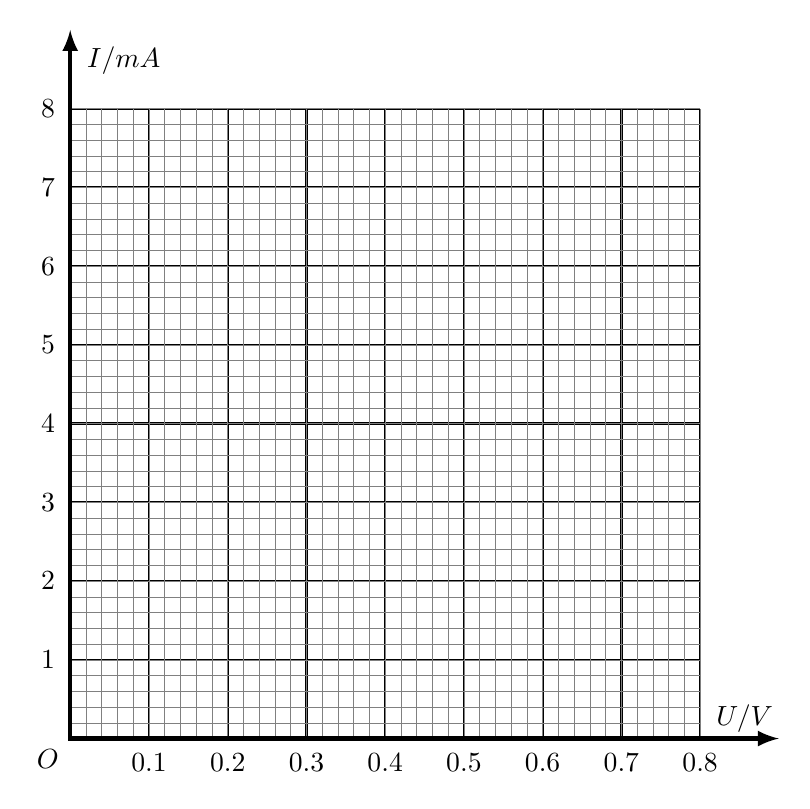
\begin{tikzpicture}
\draw[thick] (0,0) grid (8,8);
\draw[step=0.2cm,gray,very thin] (0,0) grid (8,8);

\draw[ultra thick,latex-latex] (9,0) node [above left=-2pt] {$ U/V $} -- (0,0) node [below left ] {$ O $} -- (0,9) node [below right=2pt] {$ I/mA $} ;



\foreach \label in {1,2,...,8}
{
\node[below=2pt] (ww) at (\label cm , 0) {$ 0.\label $}	;
\node[left=2pt] (ww) at (0, \label cm) {$ \label $}	;
}


\end{tikzpicture}
\end{figure}

\item 
根据作出的 $ I-U $ 图线可知,该元件是 \underlinegap (选填“线性”或“非线性”)元件.
\item 
在上述测量中,如果用导线代替电路中的定值电阻 $ R_{0} $,会导致的两个后果是 \underlinegap 。
\fourchoices
{电压和电流的测量误差增大}
{可能因电流过大烧坏待测元件}
{滑动变阻器允许的调节范围变小}
{待测元件两端电压的可调节范围变小}


\end{enumerate}


\tk{
\begin{enumerate}
\item
如图
\begin{center}
\includesvg[width=0.93\linewidth]{picture/svg/GZ-3-tiyou-0675} 
\end{center}
\item 
如图
\begin{center}
\includesvg[width=0.93\linewidth]{picture/svg/GZ-3-tiyou-0676} 
\end{center}
\item 
非线性
\item 
BC
\end{enumerate}
} 





\item
疫情期间“停课不停学”
,小明同学在家自主开展实验探究.用手机拍摄物体自由下落的视频,
得到分帧图片,利用图片中小球的位置来测量当地的重力加速度,实验装置如图$ a $所示.
\begin{figure}[h!]
\centering
\begin{subfigure}{0.35\linewidth}
\centering
\includesvg[width=0.7\linewidth]{picture/svg/GZ-3-tiyou-0669} 
\caption{}\label{}
\end{subfigure}
\begin{subfigure}{0.55\linewidth}
\centering
\includesvg[width=0.96\linewidth]{picture/svg/GZ-3-tiyou-0670} 
\caption{}\label{}
\end{subfigure}
\end{figure}
\begin{enumerate}
\item
家中有乒乓球、小塑料球和小钢球,其中最适合用作实验中下落物体的是 \underlinegap .
\item 
下列主要操作步骤的正确顺序是 \underlinegap .(填写各步骤前的序号)

①把刻度尺竖直固定在墙上

②捏住小球,从刻度尺旁静止释放

③手机固定在三角架上,调整好手机镜头的位置

④打开手机摄像功能,开始摄像

\item 
停止摄像,从视频中截取三帧图片,图片中的小球和刻度如图$ 2 $所示.已知所截取的图片相邻两
帧之间的时间间隔为 $ \frac{ 1 }{ 6 } \ s $,刻度尺的分度值是 $ 1 \ mm $,由此测得重力加速度为 \underlinegap $ m/s^{2} $.

\item 
在某次实验中,小明释放小球时手稍有晃动,视频显示小球下落时偏离了竖直方向.从该视频中截取图
片, \underlinegap (选填“仍能”或“不能”)用($ 3 $)问中的方法测出重力加速度.

\end{enumerate}


\tk{
\begin{enumerate}
\item
小钢球 
\item 
①③④② 
\item 
$ 9.6 $($ 9.5 \sim 9.7 $都算对) 
\item 
仍能	
\end{enumerate}
} 








\gaokaoxx{$ 3-5 $}



\item 
\begin{enumerate}
\item
“测温枪”
(学名“红外线辐射测温仪”)具有响应快、非接触和操作方便等优点.它是根据黑体辐射规
律设计出来的,能将接收到的人体热辐射转换成温度显示.若人体温度升高,则人体热辐射强度 $ I $ 及其极大
值对应的波长 $ \lambda $ 的变化情况是 \underlinegap .
\fourchoices
{$ I $增大, $ \lambda $ 增大}
{$ I $ 增大, $ \lambda $ 减小}
{$ I $ 减小, $ \lambda $ 增大}
{$ I $ 减小, $ \lambda $ 减小}

\tk{B} 





\item 
大量处于某激发态的氢原子辐射出多条谱线,其中最长和最短波长分别为 $ \lambda_{1} $ 和 $ \lambda_{2} $,则该激发态与基
态的能量差为 \underlinegap ,波长为 $ \lambda_{1} $ 的光子的动量为 \underlinegap .(已知普朗克常量为 $ h $,光速为 $ c $)

\tk{$\frac{h c}{\lambda_{2}} \quad \frac{h}{\lambda_{1}}$} 





\item 
一只质量为 $ 1.4 \ kg $ 的乌贼吸入 $ 0.1 \ kg $ 的水,静止在水中.遇到危险时,它在极短时间内把吸入的水向后
全部喷出,以 $ 2 \ m/s $ 的速度向前逃窜.求该乌贼喷出的水的速度大小 $ v $.

\banswer{
$v=28 \ m / s$
}





\end{enumerate}









\newpage

\gaokaoxx{$ 3-3 $}

\item 
\begin{enumerate}
\item
玻璃的出现和使用在人类生活里已有四千多年的历史,它是一种非晶体.下列关于玻璃的说法正确的有 \underlinegap .
\fourchoices
{没有固定的熔点}
{天然具有规则的几何形状}
{沿不同方向的导热性能相同}
{分子在空间上周期性排列}

\tk{AC} 





\item 
一瓶酒精用了一些后,把瓶盖拧紧,不久瓶内液面上方形成了酒精的饱和汽,此时 \underlinegap (选填“有”
或“没有”
)酒精分子从液面飞出.当温度升高时,瓶中酒精饱和汽的密度 \underlinegap (选填“增大”
“减小”或“不
变”).

\tk{有 \quad 增大} 





\item 
一定质量的理想气体从状态 $ A $ 经状态 $ B $ 变化到状态 $ C $,其 $ p-\frac{1}{V} $
图象如图所示,求该过程中气体吸收
的热量 $ Q $.
\begin{figure}[h!]
\flushright
\includesvg[width=0.25\linewidth]{picture/svg/GZ-3-tiyou-0671}
\end{figure}

\banswer{
$Q=2 \times 10^{5} \ J$
}





\end{enumerate}




\gaokaoxx{$ 3-4 $}



\item 

\begin{enumerate}
\item
电磁波广泛应用在现代医疗中.下列属于电磁波应用的医用器械有 \underlinegap .
\fourchoices
{杀菌用的紫外灯}
{拍胸片的 $ X $ 光机}
{治疗咽喉炎的超声波雾化器}
{检查血流情况的“彩超”机}

\tk{AB} 





\item 
我国的光纤通信技术处于世界领先水平.光纤内芯(内层玻璃)的折射率比外套(外层玻璃)的
\underlinegap (选填“大”或“小”
).某种光纤的内芯在空气中全反射的临界角为 $ 43 ^{ \circ } $,则该内芯的折射率为 \underlinegap .(取
$ \sin 43 ^{ \circ } =0.68, \cos 43 ^{ \circ } =0.73 $,结果保留 $ 2 $ 位有效数字)


\tk{大 \quad 1.5} 





\item 
国际宇航联合会将 $ 2020 $ 年度“世界航天奖”授予我国“嫦娥四号”任务团队.“嫦娥四号”任务创造
了多项世界第一.在探月任务中,
“玉兔二号”月球车朝正下方发射一束频率为 $ f $ 的电磁波,该电磁波分别在
月壤层的上、下表面被反射回来,反射波回到“玉兔二号”的时间差为 $ \Delta t $.已知电磁波在月壤层中传播的波
长为 $ \lambda $,求该月壤层的厚度 $ d $.

\banswer{
$d=\frac{f \lambda \Delta t}{2}$
}





\end{enumerate}



\gaokaojs



\item
如图所示,电阻为 $ 0.1 \ \Omega $ 的正方形单匝线圈 $ abcd $ 的边长为 $ 0.2 \ m $, $ bc $ 边与匀强磁场边缘重合.
磁场的宽度等于线圈的边长,磁感应强度大小为 $ 0.5 \ T $.在水平拉力作用下,线圈以 $ 8 \ m/s $ 的速度向右穿过磁
场区域.求线圈在上述过程中:
\begin{enumerate}
\item
感应电动势的大小 $ E $;
\item 
所受拉力的大小 $ F $;
\item 
感应电流产生的热量 $ Q $.

\end{enumerate}
\begin{figure}[h!]
\flushright
\includesvg[width=0.33\linewidth]{picture/svg/GZ-3-tiyou-0672}
\end{figure}

\banswer{
\begin{enumerate}
\item
$E=0.8 \ V$	
\item 	
$F=0.8 \ N$
\item 
$Q=0.32 \ J$	
\end{enumerate}
}





\item
如图所示,鼓形轮的半径为 $ R $,可绕固定的光滑水平轴 $ O $ 转动.在轮上沿相互垂直的直径方向固
定四根直杆,杆上分别固定有质量为 $ m $ 的小球,球与 $ O $ 的距离均为 $ 2R $.在轮上绕有长绳,绳上悬挂着质量
为 $ M $ 的重物.重物由静止下落,带动鼓形轮转动.重物落地后鼓形轮匀速转动,转动的角速度为 $ \omega $.绳与轮之
间无相对滑动,忽略鼓形轮、直杆和长绳的质量,不计空气阻力,重力加速度为 $ g $.求:
\begin{enumerate}
\item
重物落地后,小球线速度的大小 $ v $;
\item 
重物落地后一小球转到水平位置 $ A $,此时该球受到杆的作用力的大小 $ F $;
\item 
重物下落的高度 $ h $.
\end{enumerate}
\begin{figure}[h!]
\flushright
\includesvg[width=0.25\linewidth]{picture/svg/GZ-3-tiyou-0673}
\end{figure}



\banswer{
\begin{enumerate}
\item
$v=2 \omega R$	
\item 
$F=\sqrt{\left(2 m \omega^{2} R\right)^{2}+(m g)^{2}}$
\item 
$h=\frac{M+16 m}{2 M g}(\omega R)^{2}$
\end{enumerate}
}






\newpage

\item
空间存在两个垂直于 $ Oxy $ 平面的匀强磁场,$ y $ 轴为两磁场的边界,磁感应强度分别为 $ 2B_{0} $、$ 3B_{0} $.
甲、乙两种比荷不同的粒子同时从原点 $ O $ 沿 $ x $ 轴正向射入磁场,速度均为 $ v $.甲第 $ 1 $ 次、第 $ 2 $ 次经过 $ y $ 轴的
位置分别为 $ P $、$ Q $,其轨迹如图所示.甲经过 $ Q $ 时,乙也恰好同时经过该点.已知甲的质量为 $ m $,电荷量为 $ q $.
不考虑粒子间的相互作用和重力影响.求:
\begin{enumerate}
\item
$ Q $ 到 $ O $ 的距离 $ d $;
\item 
甲两次经过 $ P $ 点的时间间隔 $ \Delta t $;
\item 
乙的比荷$ \frac{q}{m} $可能的最小值.
\end{enumerate}
\begin{figure}[h!]
\flushright
\includesvg[width=0.28\linewidth]{picture/svg/GZ-3-tiyou-0674}
\end{figure}



\banswer{
\begin{enumerate}
\item
$d=\frac{m v}{3 q B_{0}}$
\item 
$\Delta t=\frac{2 \pi m}{q B_{0}}$
\item 
比荷的最小值为 $\frac{2 q}{m}$
\end{enumerate}
}





\end{enumerate}

%

\gaokaoheader{2020}{山东卷}


\gaokaoxz


\begin{enumerate}
\item
一质量为 $ m $ 的乘客乘坐竖直电梯下楼,其位移 $ s $ 与时间 $ t $ 的关系图像如图所示。乘客所受支持力的大小
用 $ F_{N} $ 表示,速度大小用 $ v $ 表示。重力加速度大小为 $ g $。以下判断正确的是 \xzanswer{D} 
\begin{figure}[h!]
\centering
\includesvg[width=0.23\linewidth]{picture/svg/GZ-3-tiyou-0729}
\end{figure}


\fourchoices
{$ 0 \sim t_{1} $ 时间内,$ v $ 增大,$ F_{N} >mg $}
{$ t_{1} \sim t_{2} $ 时间内,$ v $ 减小,$ F_{N} <mg $}
{$ t_{2} \sim t_{3} $ 时间内,$ v $ 增大,$ F_{N} <mg $}
{$ t_{2} \sim t_{3} $ 时间内,$ v $ 减小,$ F_{N} >mg $}





\item
氚核 \ce{^{3}_{1}H} 发生$ \beta $衰变成为氦核 \ce{^{3}_{2}He} 。假设含氚材料中 \ce{^{3}_{2}He} 发生$ \beta $衰变产生的电子可以全部定向移动,在 $ 3.2 \times 10^{4} \ s $ 时间内形成的平均电流为 $ 5.0 \times 10^{-8} \ A $。已知电子电荷量为 $ 1.6 \times 10^{-19} \ C $,在这段时间内发生$ \beta $衰变的
氚核 \ce{^{3}_{1}H} 的个数为 \xzanswer{B} 

\fourchoices
{$5.0 \times 10^{14}$}
{$1.0 \times 10^{16}$}
{$ 2.0 \times 10^{16}$}
{$1.0 \times 10^{18}$}






\item
双缝干涉实验装置的截面图如图所示。光源 $ S $ 到 $ S_{1} $、$ S_{2} $ 的距离相等,$ O $ 点为 $ S_{1} $、$ S_{2} $ 连线中垂线与光屏的
交点。光源 $ S $ 发出的波长为 $ \lambda $ 的光,经 $ S_{1} $ 出射后垂直穿过玻璃片传播到 $ O $ 点,经 $ S_{2} $ 出射后直接传播到
$ O $ 点,由 $ S_{1} $ 到 $ O $ 点与由 $ S_{2} $ 到 $ O $ 点,光传播的时间差为 $ \Delta t $。玻璃片厚度为 $ 10\lambda $,玻璃对该波长光的折射
率为 $ 1.5 $,空气中光速为 $ c $,不计光在玻璃片内的反射。以下判断正确的是 \xzanswer{A} 
\begin{figure}[h!]
\centering
\includesvg[width=0.3\linewidth]{picture/svg/GZ-3-tiyou-0730}
\end{figure}


\fourchoices
{$\Delta t=\frac{5 \lambda}{c}$}
{$ \Delta t=\frac{15 \lambda}{2 c}$}
{$ \Delta t=\frac{10 \lambda}{c}$}
{$ \Delta t=\frac{15 \lambda}{c}$}





\item
一列简谐横波在均匀介质中沿 $ x $ 轴负方向传播,
已知 $ x= \frac{ 5 }{ 4 } \lambda $ 处质点的振动方程为 $y=A \cos \left(\frac{2 \pi}{T} t\right)$,
则$ t= \frac{ 3 }{ 4 } T $
时刻的波形图正确的是 \xzanswer{D} 

\pfourchoices
{\includesvg[width=3.3cm]{picture/svg/GZ-3-tiyou-0731}}
{\includesvg[width=3.3cm]{picture/svg/GZ-3-tiyou-0732}}
{\includesvg[width=3.3cm]{picture/svg/GZ-3-tiyou-0733}}
{\includesvg[width=3.3cm]{picture/svg/GZ-3-tiyou-0734}}







\item
图 \subref{2020:山东:5a} 中的理想变压器原、副线圈匝数比 $ n_{1}:n_{2}=22:3 $,输入端 $ a $、$ b $ 所接电压 $ u $ 随时间 $ t $ 的变化关系如图 \subref{2020:山东:5b} 所示。灯泡 $ L $ 的电阻恒为 $ 15 \ \Omega $,额定电压为 $ 24 \ V $。定值电阻 $ R_{1} =10 \ \Omega $、$ R_{2} =5 \ \Omega $, 滑动变阻器 $ R $ 的最
大阻值为 $ 10 \ \Omega $。为使灯泡正常工作,滑动变阻器接入电路的电阻应调节为 \xzanswer{A} 

\begin{figure}[h!]
\centering
\begin{subfigure}{0.4\linewidth}
\centering
\includesvg[width=0.8\linewidth]{picture/svg/GZ-3-tiyou-0735} 
\caption{}\label{2020:山东:5a}
\end{subfigure}
\begin{subfigure}{0.4\linewidth}
\centering
\includesvg[width=0.8\linewidth]{picture/svg/GZ-3-tiyou-0736} 
\caption{}\label{2020:山东:5b}
\end{subfigure}	
\end{figure}


\fourchoices
{$ 1 \ \Omega $}
{$ 5 \ \Omega $}
{$ 6 \ \Omega $}
{$ 8 \ \Omega $}





\item
一定质量的理想气体从状态 $ a $ 开始,经 $ a \rightarrow b $、$ b \rightarrow c $、$ c \rightarrow a $ 三个过程后回到初始状态 $ a $,其 $ p-V $ 图像如图
所示。已知三个状态的坐标分别为 $ a $($ V_{0} $, $ 2p_0 $)、 $ b $($ 2V_0 $,$ p_{0} $)、$ c $($ 3V_0 $, $ 2p_0 $) 以下判断正确的是 \xzanswer{C} 
\begin{figure}[h!]
\centering
\includesvg[width=0.26\linewidth]{picture/svg/GZ-3-tiyou-0737}
\end{figure}


\fourchoices
{气体在 $ a \rightarrow b $ 过程中对外界做的功小于在 $ b \rightarrow c $ 过程中对外界做的功}
{气体在 $ a \rightarrow b $ 过程中从外界吸收的热量大于在 $ b \rightarrow c $ 过程中从外界吸收的热量}
{在 $ c \rightarrow a $ 过程中,外界对气体做的功小于气体向外界放出的热量}
{气体在 $ c \rightarrow a $ 过程中内能的减少量大于 $ b \rightarrow c $ 过程中内能的增加量}





\item
我国将在今年择机执行“天问 $ 1 $ 号”火星探测任务。质量为 $ m $ 的着陆器在着陆火星前,会在火星表面附近
经历一个时长为 $ t_{0} $、速度由 $ v_{0} $ 减速到零的过程。已知火星的质量约为地球的 $ 0.1 $ 倍,半径约为地球的 $ 0.5 $倍,地球表面的重力加速度大小为 $ g $,忽略火星大气阻力。若该减速过程可视为一个竖直向下的匀减
速直线运动,此过程中着陆器受到的制动力大小约为 \xzanswer{B} 

\fourchoices
{$m\left(0.4 g-\frac{v_{0}}{t_{0}}\right)$}
{$ m\left(0.4 g+\frac{v_{0}}{t_{0}}\right)$}
{$ m\left(0.2 g-\frac{v_{0}}{t_{0}}\right)$}
{$ m\left(0.2 g+\frac{v_{0}}{t_{0}}\right)$}






\item
如图所示,一轻质光滑定滑轮固定在倾斜木板上,质量分别为 $ m $ 和 $ 2m $ 的物块 $ A $、$ B $,通过不可伸长的轻
绳跨过滑轮连接,$ A $、$ B $ 间的接触面和轻绳均与木板平行。$ A $ 与 $ B $ 间、$ B $ 与木板间的动摩擦因数均为$ \mu $,
设最大静摩擦力等于滑动摩擦力。当木板与水平面的夹角为 $ 45 ^{ \circ } $时,物块 $ A $、$ B $ 刚好要滑动,则$ \mu $的值为 \xzanswer{C} 
\begin{figure}[h!]
\centering
\includesvg[width=0.27\linewidth]{picture/svg/GZ-3-tiyou-0738}
\end{figure}

\fourchoices
{$\frac{1}{3}$}
{$\frac{1}{4}$}
{$\frac{1}{5}$}
{$\frac{1}{6}$}








\item
截面为等腰直角三角形的三棱镜如图 \subref{2020:山东:9a} 所示。$ DE $ 为嵌在三棱镜内部紧贴 $ BB ^{\prime} C ^{\prime} C $ 面的线状单色可见光光
源,$ DE $ 与三棱镜的 $ ABC $ 面垂直,$ D $ 位于线段 $ BC $ 的中点。图 \subref{2020:山东:9b} 为图 \subref{2020:山东:9a} 中 $ ABC $ 面的正视图。三棱镜对
该单色光的折射率为 $ 2 $,只考虑由 $ DE $ 直接射向侧面 $ AA ^{\prime} C ^{\prime} C $ 的光线。下列说法正确的是 \xzanswer{AC} 
\begin{figure}[h!]
\centering
\begin{subfigure}{0.3\linewidth}
\centering
\includesvg[width=0.8\linewidth]{picture/svg/GZ-3-tiyou-0739} 
\caption{}\label{2020:山东:9a}
\end{subfigure}
\begin{subfigure}{0.3\linewidth}
\centering
\includesvg[width=0.8\linewidth]{picture/svg/GZ-3-tiyou-0740} 
\caption{}\label{2020:山东:9b}
\end{subfigure}
\end{figure}


\fourchoices
{光从 $ AA ^{\prime} C ^{\prime} C $ 面出射的区域占该侧面总面积的$ \frac{ 1 }{ 2 } $}
{光从 $ AA ^{\prime} C ^{\prime} C $ 面出射的区域占该侧面总面积的$ \frac{ 2 }{ 3 } $}
{若 $ DE $ 发出的单色光频率变小,$ AA ^{\prime} C ^{\prime} C $ 面有光出射的区域面积将增大}
{若 $ DE $ 发出的单色光频率变小,$ AA ^{\prime} C ^{\prime} C $ 面有光出射的区域面积将减小}





\item
真空中有两个固定的带正电的点电荷,电荷量不相等。一个带负电的试探电荷置于二者连线上的 $ O $ 点
时,仅在电场力的作用下恰好保持静止状态。过 $ O $ 点作两正电荷连线的垂线,以 $ O $ 点为圆心的圆与连
线和垂线分别交于 $ a $、$ c $ 和 $ b $、$ d $,如图所示。以下说法正确的是 \xzanswer{BD} 
\begin{figure}[h!]
\centering
\includesvg[width=0.39\linewidth]{picture/svg/GZ-3-tiyou-0741}
\end{figure}


\fourchoices
{$ a $ 点电势低于 $ O $ 点}
{$ b $ 点电势低于 $ c $ 点}
{该试探电荷在 $ a $ 点的电势能大于在 $ b $ 点的电势能}
{该试探电荷在 $ c $ 点的电势能小于在 $ d $ 点的电势能}






\item
如图所示,质量为 $ M $ 的物块 $ A $ 放置在光滑水平桌面上,右侧连接一固定于墙面的水平轻绳,左侧通过
一倾斜轻绳跨过光滑定滑轮与一竖直轻弹簧相连。现将质量为 $ m $ 的钩码 $ B $ 挂于弹簧下端,当弹簧处于
原长时,将 $ B $ 由静止释放,当 $ B $ 下降到最低点时(未着地),$ A $ 对水平桌面的压力刚好为零。轻绳不
可伸长,弹簧始终在弹性限度内,物块 $ A $ 始终处于静止状态。以下判断正确的是 \xzanswer{ACD} 
\begin{figure}[h!]
\centering
\includesvg[width=0.28\linewidth]{picture/svg/GZ-3-tiyou-0742}
\end{figure}


\fourchoices
{$ M<2m $}
{$ 2m<M<3 \ m $}
{在 $ B $ 从释放位置运动到最低点的过程中,所受合力对 $ B $ 先做正功后做负功}
{在 $ B $ 从释放位置运动到速度最大的过程中,$ B $ 克服弹簧弹力做的功等于 $ B $ 机械能的减少量}






\item 
如图所示,平面直角坐标系的第一和第二象限分别存在磁感应强度大小相等、方向相反且垂直于坐标
平面的匀强磁场,图中虚线方格为等大正方形。一位于 $ Oxy $ 平面内的刚性导体框 $ abcde $ 在外力作用下
以恒定速度沿 $ y $ 轴正方向运动(不发生转动)。从图示位置开始计时,$ 4 \ s $ 末 $ bc $ 边刚好进入磁场。在
此过程中,导体框内感应电流的大小为 $ I $ , $ ab $ 边所受安培力的大小为 $ F_{ab} $,二者与时间 $ t $ 的关系图像,
可能正确的是 \xzanswer{BC} 
\begin{figure}[h!]
\centering
\includesvg[width=0.28\linewidth]{picture/svg/GZ-3-tiyou-0743}
\end{figure}

\pfourchoices
{\includesvg[width=3cm]{picture/svg/GZ-3-tiyou-0744}}
{\includesvg[width=3cm]{picture/svg/GZ-3-tiyou-0745}}
{\includesvg[width=3cm]{picture/svg/GZ-3-tiyou-0746}}
{\includesvg[width=3cm]{picture/svg/GZ-3-tiyou-0747}}









\gaokaosy

\item
$ 2020 $ 年 $ 5 $ 月,我国进行了珠穆朗玛峰的高度测量,其中一种方法是通过使用重力仪测量重力
加速度,进而间接测量海拔高度。某同学受此启发就地取材设计了如下实验,测量当地重力加速度的
大小。实验步骤如下:
\begin{figure}[h!]
\centering
\begin{subfigure}{0.4\linewidth}
\centering
\includesvg[width=0.7\linewidth]{picture/svg/GZ-3-tiyou-0748} 
\caption{}\label{2020:山东:13a}
\end{subfigure}
\begin{subfigure}{0.8\linewidth}
\centering
\includesvg[width=0.8\linewidth]{picture/svg/GZ-3-tiyou-0749} 
\caption{}\label{2020:山东:13b}
\end{subfigure}
\end{figure}

\begin{enumerate}
\renewcommand{\labelenumii}{\roman{enumii}.}
\item
如图 \subref{2020:山东:13a} 所示,选择合适高度的垫块,使木板的倾角为 $ 53 ^{ \circ } $,在其上表面固定一与小物块下滑路径平行的刻度尺(图中未画出)。
\item 
调整手机使其摄像头正对木板表面,开启视频录像功能。将小物块从木板顶端释放,用手机记录
下小物块沿木板向下做加速直线运动的情况。然后通过录像的回放,选择小物块运动路径上合适的一
点作为测量参考点,得到小物块相对于该点的运动距离 $ L $ 与运动时间 $ t $ 的数据。
\item 
该同学选取部分实验数据,画出了$\frac{2 L}{t}-t$图像,利用图像数据得到小物块下滑的加速度大小为 $ 5.6 \ m/s^{2} $。
\item 
再次调节垫块,改变木板的倾角,重复实验。

\end{enumerate}


回答以下问题:
\begin{enumerate}
\item
当木板的倾角为 $ 37 ^{ \circ } $时,所绘图像如图 \subref{2020:山东:13b} 所示。由图像可得,物块过测量参考点时速度的大小为 \underlinegap 
$ m/s $;选取图线上位于坐标纸网格交叉点上的 $ A $、$ B $ 两点,利用 $ A $、$ B $ 两点数据得到小物块下滑加速
度的大小为 \underlinegap $ m/s^{2} $。(结果均保留 $ 2 $ 位有效数字)


\item 
根据上述数据,进一步分析得到当地的重力加速度大小为 \underlinegap $ m/s^{2} $。(结果保留 $ 2 $ 位有效数字,$ \sin 37 ^{ \circ } =0.60 $,$ \cos 37 ^{ \circ } =0.80 $ )


\end{enumerate}

\tk{
\begin{enumerate}
\item 
$ 0.32 $或$ 0.33 $\quad$ 3.1 $ 
\item 
$ 9.4 $	
\end{enumerate}
} 







\item
实验方案对实验测量的精度有直接的影响,某学习小组对“测量电源的电动势和内阻”的实验方
案进行了探究。实验室提供的器材有:

干电池一节(电动势约 $ 1.5 \ V $,内阻小于 $ 1 \ \Omega $);


电压表 $ V $ (量程 $ 3 \ V $,内阻约 $ 3 \ k\Omega $);


电流表 $ A $ (量程 $ 0.6 \ A $,内阻约 $ 1 \ \Omega $);


滑动变阻器 $ R $ (最大阻值为 $ 20 \ \Omega $);


定值电阻 $ R_{1} $ (阻值 $ 2 \ \Omega $);


定值电阻 $ R_{2} $ (阻值 $ 5 \ \Omega $);

开关一个,导线若干。

\begin{enumerate}
\item
该小组按照图 \subref{2020:山东:14a} 所示的电路进行实验,通过调节滑动变阻器阻值使电流表示数逐渐接近满偏,记
录此过程中电压表和电流表的示数,利用实验数据在 $ U-I $ 坐标纸上描点,如图 \subref{2020:山东:14b} 所示,结果发现电压表
示数的变化范围比较小,出现该现象的主要原因是 \underlinegap 。(单选,填正确答案标号)
\fourchoices
{电压表分流}
{干电池内阻较小}
{滑动变阻器最大阻值较小}
{电流表内阻较小}
\begin{figure}[h!]
\centering
\begin{subfigure}{0.4\linewidth}
\centering
\includesvg[width=0.7\linewidth]{picture/svg/GZ-3-tiyou-0750} 
\caption{}\label{2020:山东:14a}
\end{subfigure}
\begin{subfigure}{0.5\linewidth}
\centering
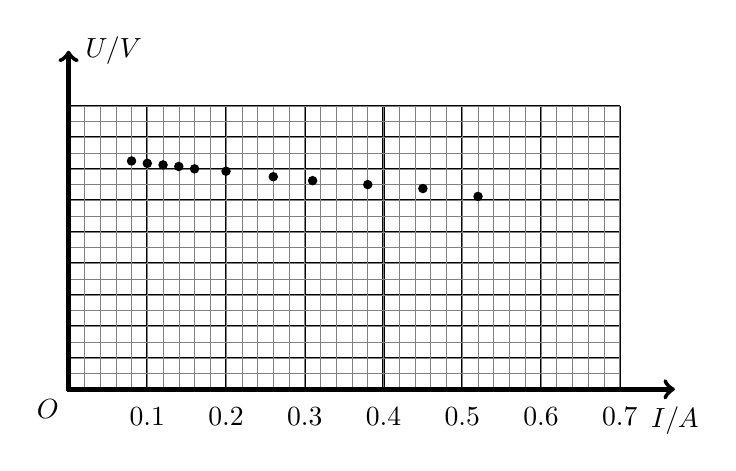
\begin{tikzpicture}
\draw[thick,xstep=1cm,ystep=0.4cm] (0,0) grid (7,3.6); %主网格
\draw[step=0.2cm,gray,very thin] (0,0) grid (7,3.6);%次网格

\draw[ultra thick,->] (-0.02,0) -- (7.7,0) node [below =2pt] {$ I/A $} ; %横坐标轴
\draw[ultra thick,->] (0,-0.02) -- (0,4.3) node [right =2pt] {$ U/V $} ; %纵坐标轴
\node at (0,0) [below left] {$ O $};%原点

\foreach \xlabel in {1,2,...,7}{ %x轴刻度
\node[below=3pt] at (\xlabel cm , 0) {$ 0.\xlabel $};
}
\foreach \ylabel in {0.4,0.8,1.2,1.6,2.0,2.4,2.8,3.2,3.6}{ %y轴刻度
\FPset\myy{\ylabel}%给计算的量赋值
\FPeval{myresult}{trunc(myy/2:1)}%表达式计算,\FPprint\myresult显示
\node[left=3pt] at (0, \ylabel cm) {$ \FPprint\myresult $};
}

\draw[fill] (0.8,2.9) circle [radius=1.5pt];
\draw[fill] (1.0,2.87) circle [radius=1.5pt];
\draw[fill] (1.2,2.85) circle [radius=1.5pt];
\draw[fill] (1.4,2.83) circle [radius=1.5pt];
\draw[fill] (1.6,2.80) circle [radius=1.5pt];
\draw[fill] (2,2.77) circle [radius=1.5pt];
\draw[fill] (2.6,2.7) circle [radius=1.5pt];
\draw[fill] (3.1,2.65) circle [radius=1.5pt];
\draw[fill] (3.8,2.6) circle [radius=1.5pt];
\draw[fill] (4.5,2.55) circle [radius=1.5pt];
\draw[fill] (5.2,2.45) circle [radius=1.5pt];
\end{tikzpicture}
\caption{}\label{2020:山东:14b}
\end{subfigure}
\end{figure}

\item 
针对电压表示数的变化范围比较小的问题,该小组利用实验室提供的器材改进了实验方案,重新
测量得到的数据如下表所示。

\begin{table}[h!]
\centering 
\begin{tabular}{|c|c|c|c|c|c|c|c|}
\hline 
序号 & 1 & 2 & 3 & 4 & 5 & 6 & 7
\\
\hline
$ I/A $ & 0.08 & 0.14 & 0.20 & 0.26 & 0.32 & 0.36 & 0.40
\\
\hline
$ U/V $& 1.35 & 1.20 & 1.05 & 0.88 & 0.73 & 0.71 & 0.52\\ 
\hline 
\end{tabular}
\end{table} 




请根据实验数据,回答以下问题:
\begin{enumerate}
\item
答题卡的坐标纸上已标出后 $ 3 $ 组数据对应的坐标点,请在答题卡的坐标纸上标出前 $ 4 $ 组数据对应的
坐标点并画出 $ U-I $ 图像。
\begin{figure}[h!]
\centering
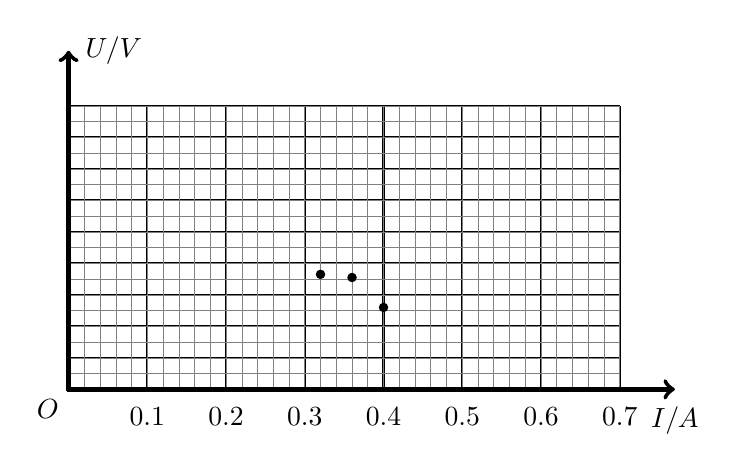
\begin{tikzpicture}
\draw[thick,xstep=1cm,ystep=0.4cm] (0,0) grid (7,3.6); %主网格
\draw[step=0.2cm,gray,very thin] (0,0) grid (7,3.6);%次网格

\draw[ultra thick,->] (-0.02,0) -- (7.7,0) node [below =2pt] {$ I/A $} ; %横坐标轴
\draw[ultra thick,->] (0,-0.02) -- (0,4.3) node [right =2pt] {$ U/V $} ; %纵坐标轴
\node at (0,0) [below left] {$ O $};%原点

\foreach \xlabel in {1,2,...,7}{ %x轴刻度
\node[below=3pt] at (\xlabel cm , 0) {$ 0.\xlabel $};
}
\foreach \ylabel in {0.4,0.8,1.2,1.6,2.0,2.4,2.8,3.2,3.6}{ %y轴刻度
\FPset\myy{\ylabel}%给计算的量赋值
\FPeval{myresult}{trunc(myy/2:1)}%表达式计算,\FPprint\myresult显示
\node[left=3pt] at (0, \ylabel cm) {$ \FPprint\myresult $};
}

\draw[fill] (4,1.04) circle [radius=1.5pt];
\draw[fill] (3.6,1.42) circle [radius=1.5pt];
\draw[fill] (3.2,1.46) circle [radius=1.5pt];
\end{tikzpicture}
\end{figure}


\item 
根据实验数据可知,所选的定值电阻为 \underlinegap (填“$ R_{1} $”或“$ R_{2} $”)。


\item 
用笔画线代替导线,请在答题卡上按照改进后的方案,将实物图连接成完整电路。
\begin{figure}[h!]
\centering
\includesvg[width=0.43\linewidth]{picture/svg/GZ-3-tiyou-1709}
\end{figure}

\end{enumerate}


\end{enumerate}


\tk{
\begin{enumerate}
\item
B	
\item 	
\begin{enumerate}
\item
如图:
\begin{center}
\includesvg[width=0.93\linewidth]{picture/svg/GZ-3-tiyou-0759} 
\end{center}
\item 
$ R_{1} $
\item 
如图:
\begin{center}
\includesvg[width=0.93\linewidth]{picture/svg/GZ-3-tiyou-1708} 
\end{center}
\end{enumerate}
\end{enumerate}
} 




\newpage
\gaokaojs

\item
中医拔罐的物理原理是利用玻璃罐内外的气压差使罐吸附在人体穴位上,进而治疗某些疾病。
常见拔罐有两种,如图所示,左侧为火罐,下端开口;右侧为抽气拔罐,下端开口,上端留有抽气阀
门。使用火罐时,先加热罐中气体,然后迅速按到皮肤上,自然降温后火罐内部气压低于外部大气压,
使火罐紧紧吸附在皮肤上。抽气拔罐是先把罐体按在皮肤上,再通过抽气降低罐内气体压强。某次使
用火罐时,罐内气体初始压强与外部大气压相同,温度为 $ 450 \ K $,最终降到 $ 300 \ K $,因皮肤凸起,内
部气体体积变为罐容积的$ \frac{20}{21} $。若换用抽气拔罐,抽气后罐内剩余气体体积变为抽气拔罐容积的$ \frac{20}{21} $,
罐内气压与火罐降温后的内部气压相同。罐内气体均可视为理想气体,忽略抽气过程中气体温度的变
化。求应抽出气体的质量与抽气前罐内气体质量的比值。
\begin{figure}[h!]
\flushright
\includesvg[width=0.35\linewidth]{picture/svg/GZ-3-tiyou-0752}
\end{figure}


\banswer{
$\frac{\Delta m}{m}=\frac{1}{3}$
}



\newpage
\item 
单板滑雪 $ U $ 型池比赛是冬奥会比赛项目,其场地可以简化为如图 \subref{2020:山东:16a} 所示的模型$ :U $ 形滑道由两
个半径相同的四分之一圆柱面轨道和一个中央的平面直轨道连接而成,轨道倾角为 $ 17.2 ^{ \circ } $。某次练习
过程中,运动员以 $ v_{M}=10 \ m/s $ 的速度从轨道边缘上的 $ M $ 点沿轨道的竖直切面 $ ABCD $ 滑出轨道,速度方
向与轨道边缘线 $ AD $ 的夹角$ \alpha =72.8 ^{ \circ } $,腾空后沿轨道边缘的 $ N $ 点进入轨道。图 \subref{2020:山东:16b} 为腾空过程左视图。
该运动员可视为质点,不计空气阻力,取重力加速度的大小 $ g=10 \ m/s^{2}, \sin 72.8 ^{ \circ } =0.96 $,$ \cos 72.8 ^{ \circ } =0.30$。求:
\begin{enumerate}
\item
运动员腾空过程中离开 $ AD $ 的距离的最大值 $ d $;
\item 
$ M $、$ N $ 之间的距离 $ L $。
\end{enumerate}
\begin{figure}[h!]
\flushright
\begin{subfigure}{0.4\linewidth}
\centering
\includesvg[width=0.85\linewidth]{picture/svg/GZ-3-tiyou-0754} 
\caption{}\label{2020:山东:16a}
\end{subfigure}
\begin{subfigure}{0.4\linewidth}
\centering
\includesvg[width=0.95\linewidth]{picture/svg/GZ-3-tiyou-0755} 
\caption{}\label{2020:山东:16b}
\end{subfigure}
\end{figure}



\banswer{
\begin{enumerate}
\item
$d=4.8 \ m$	
\item 
$L=12 \ m$
\end{enumerate}
}






\newpage
\item
某型号质谱仪的工作原理如图 \subref{2020:山东:17a} 所示。$ M $、$ N $ 为竖直放置的两金属板,两板间电压为 $ U,Q $ 板
为记录板,分界面 $ P $ 将 $ N $、$ Q $ 间区域分为宽度均为 $ d $ 的 \lmd{1} 、 \lmd{1} 两部分,$ M $、$ N $、$ P $、$ Q $ 所在平面相互平行,
$ a $、$ b $ 为 $ M $、$ N $ 上两正对的小孔。以 $ a $、$ b $ 所在直线为 $ z $ 轴, 向右为正方向,取 $ z $ 轴与 $ Q $ 板的交点 $ O $ 为坐
标原点,以平行于 $ Q $ 板水平向里为 $ x $ 轴正方向,竖直向上为 $ y $ 轴正方向,建立空间直角坐标系 $ Oxyz $。
区域 \lmd{1} 、$ \lmd{2} $内分别充满沿 $ x $ 轴正方向的匀强磁场和匀强电场,磁感应强度大小、电场强度大小分别为 $ B $和 $ E $。一质量为 $ m $,电荷量为$ +q $ 的粒子,从 $ a $ 孔飘入电场(初速度视为零),经 $ b $ 孔进入磁场,过 $ P $ 面
上的 $ c $ 点(图中未画出)进入电场,最终打到记录板 $ Q $ 上。不计粒子重力。
\begin{enumerate}
\item
求粒子在磁场中做圆周运动的半径 $ R $ 以及 $ c $ 点到 $ z $ 轴的距离 $ L $;
\item 
求粒子打到记录板上位置的 $ x $ 坐标;
\item 
求粒子打到记录板上位置的 $ y $ 坐标(用 $ R $、$ d $ 表示);
\item 
如图 \subref{2020:山东:17b} 所示,在记录板上得到三个点 $ s_{1} $、$ s_{2} $、$ s_{3} $,若这三个点是质子 \ce{^{1}_{1}H} 、氚核 \ce{^{3}_{1}H} 、氦核 \ce{^{4}_{2}He} 的位
置,请写出这三个点分别对应哪个粒子(不考虑粒子间的相互作用,不要求写出推导过程)。

\end{enumerate}
\begin{figure}[h!]
\flushright
\begin{subfigure}{0.4\linewidth}
\centering
\includesvg[width=0.8\linewidth]{picture/svg/GZ-3-tiyou-0756} 
\caption{}\label{2020:山东:17a}
\end{subfigure}
\begin{subfigure}{0.4\linewidth}
\centering
\includesvg[width=0.6\linewidth]{picture/svg/GZ-3-tiyou-0757} 
\caption{}\label{2020:山东:17b}
\end{subfigure}	
\end{figure}


\banswer{
\begin{enumerate}
\item
$R=\frac{\sqrt{2 m q U}}{q B}$ \quad $L=\frac{\sqrt{2 m q U}}{q B}-\sqrt{\frac{2 m U}{q B^{2}}-d^{2}}$
\item 
$x=\frac{m d^{2} E}{4 m U-2 q d^{2} B^{2}}$
\item 
$y=R-\sqrt{R^{2}-d^{2}}+\frac{d^{2}}{\sqrt{R^{2}-d^{2}}}$
\item 
$s_{1} $、$ s_{2}$、$ s_{3}$ 分别对应气核 ${ }_{1}^{3} \mathrm{H}$、氦去 ${ }_{2}^{4} \mathrm{He}$、质子 ${ }^{1}_{1} \mathrm{H}$ 的位置
\end{enumerate}
}





\newpage
\item
如图所示,一倾角为$ \theta $的固定斜面的底端安装一弹性挡板,$ P $、$ Q $ 两物块的质量分别为 $ m $ 和
$ 4m $,$ Q $ 静止于斜面上 $ A $ 处。某时刻,$ P $ 以沿斜面向上的速度 $ v_{0} $ 与 $ Q $ 发生弹性碰撞。$ Q $ 与斜面间的动摩
擦因数等于 $ \tan \theta $,设最大静摩擦力等于滑动摩擦力。$ P $ 与斜面间无摩擦,与挡板之间的碰撞无动能损
失。两物块均可以看作质点,斜面足够长,$ Q $ 的速度减为零之前 $ P $ 不会与之发生碰撞。重力加速度大
小为 $ g $。
\begin{enumerate}
\item
求 $ P $ 与 $ Q $ 第一次碰撞后瞬间各自的速度大小 $ v _{P1} $、$ v _{Q1} $;
\item 
求第 $ n $ 次碰撞使物块 $ Q $ 上升的高度 $ h_n $;
\item 
求物块 $ Q $ 从 $ A $ 点上升的总高度 $ H $;
\item 
为保证在 $ Q $ 的速度减为零之前 $ P $ 不会与之发生碰撞,求 $ A $ 点与挡板之间的最小距离 $ s $。
\end{enumerate}
\begin{figure}[h!]
\flushright
\includesvg[width=0.4\linewidth]{picture/svg/GZ-3-tiyou-0758}
\end{figure}

\banswer{
\begin{enumerate}
\item
$v_{P 1}=-\frac{3}{5} v_{0}$ \quad 
$v_{Q 1}=\frac{2}{5} v_{0}$
\item 
$h_{1}=\frac{v_{0}^{2}}{25 g}$ \\
$h_{2}=\frac{7}{25} \cdot \frac{v_{0}^{2}}{25 g}$ \\
$h_{3}=\left(\frac{7}{25}\right)^{2} \cdot \frac{v_{0}^{2}}{25 g}$\\
总结可知,第 $n$ 次碰撞后,物块 $Q$ 上升的高度为:\\
$h_{n}=\left(\frac{7}{25}\right)^{n-1} \cdot \frac{v_{0}^{2}}{25 g} \quad(n=1,2,3 \cdots \cdots)$
\item 
$s=\frac{(8 \sqrt{7}-13) v_{0}^{2}}{200 g \sin \theta}$
\end{enumerate}	
}





\end{enumerate}

%

\gaokaoheader{2020}{天津卷}



%一、单项选择题(每小题 $ 5 $ 分,共 $ 25 $ 分。每小题给出的四个选项中,只有一个选项是正确的)

\begin{enumerate}
%\renewcommand{\labelenumi}{\arabic{enumi}.}
% A(\Alph) a(\alph) I(\Roman) i(\roman) 1(\arabic)
%设定全局标号series=example	%引用全局变量resume=example
%[topsep=-0.3em,parsep=-0.3em,itemsep=-0.3em,partopsep=-0.3em]
%可使用leftmargin调整列表环境左边的空白长度 [leftmargin=0em]
\item
在物理学发展的进程中,人们通过对某些重要物理实验的深入观察和研究,获得正确的理论认识。下列
图示的实验中导致发现原子具有核式结构的是 \xzanswer{D} 
\pfourchoices
{\includesvg[width=4cm]{picture/svg/GZ-3-tiyou-0763}}
{\includesvg[width=4cm]{picture/svg/GZ-3-tiyou-0765}}
{\includesvg[width=4cm]{picture/svg/GZ-3-tiyou-0766}}
{\includesvg[width=4cm]{picture/svg/GZ-3-tiyou-0767}}


%题目类型:选择
%题目难度:9.5
%题目区域:光学:原子物理:电磁感应
%思想方法:
%题目特征:图像选择
%题目备注:




\item
北斗问天,国之夙愿。我国北斗三号系统的收官之星是地球静止轨道卫星,其轨道半径约为地球半径的$ 7 $倍。与近地轨道卫星相比,地球静止轨道卫星 \xzanswer{A} 
% TODO: \usepackage{graphicx} required
\begin{figure}[h!]
\centering
\includegraphics[width=0.2\linewidth]{picture/screenshot053}
\end{figure}


\fourchoices
{周期大}
{线速度大}
{角速度大}
{加速度大}

%题目类型:选择
%题目难度:8.5
%题目区域:万有引力
%思想方法:
%题目特征:材料分析
%题目备注:



\item
新冠肺炎疫情突发,中华儿女风雨同舟、守望相助,筑起了抗击疫情的巍峨长城。志愿者用非接触式体
温测量仪,通过人体辐射的红外线测量体温,防控人员用紫外线灯在无人的环境下消杀病毒,为人民健康保驾护航。红外线和紫外线相比较 \xzanswer{B} 

\fourchoices
{红外线的光子能量比紫外线的大}
{真空中红外线的波长比紫外线的长}
{真空中红外线的传播速度比紫外线的大}
{红外线能发生偏振现象,而紫外线不能}

%题目类型:选择
%题目难度:8.5
%题目区域:原子物理:电磁波
%思想方法:
%题目特征:材料分析
%题目备注:



\item
一列简谐横波沿 $ x $ 轴正方向传播,周期为 $ T $, $ t=0 $ 时的波形如图所示。 $ t=\frac{T}{4} $时 \xzanswer{C} 
\begin{figure}[h!]
\centering
\includesvg[width=0.23\linewidth]{picture/svg/GZ-3-tiyou-0768}
\end{figure}

\fourchoices
{质点 $ a $ 速度方向沿 $ y $ 轴负方向}
{质点 $ b $ 沿 $ x $ 轴正方向迁移了 $ 1 \ m $}
{质点 $ c $ 的加速度为零}
{质点 $ d $ 的位移为$ -5 \ cm $}

%题目类型:选择
%题目难度:7.5
%题目区域:机械波:波的描述
%思想方法:
%题目特征:
%题目备注:




\item
水枪是孩子们喜爱的玩具,常见的气压式水枪储水罐示意如图。从储水罐充气口充入气体,达到一定压
强后,关闭充气口。扣动扳机将阀门 $ M $ 打开,水即从枪口喷出。若在水不断喷出的过程中,罐内气体温
度始终保持不变,则气体 \xzanswer{B} 
\begin{figure}[h!]
\centering
\includesvg[width=0.23\linewidth]{picture/svg/GZ-3-tiyou-0769}
\end{figure}


\fourchoices
{压强变大}
{对外界做功}
{对外界放热}
{分子平均动能变大}

%题目类型:选择
%题目难度:7
%题目区域:热学:热力学第一定律:分子动理论
%思想方法:
%题目特征:材料分析
%题目备注:





%二、不定项选择题(每小题 $ 5 $ 分,共 $ 15 $ 分。每小题给出的四个选项中,都有多个选项是正确的。全部选对的得 $ 5 $ 分,选对但不全的得 $ 3 $ 分,选错或不答的得 $ 0 $ 分)


\item
手机无线充电是比较新颖的充电方式。如图所示,电磁感应式无线充电的原理与变压器类似,通过分别安
装在充电基座和接收能量装置上的线圈,利用产生的磁场传递能量。当充电基座上的送电线圈通入正弦式
交变电流后,就会在邻近的受电线圈中感应出电流,最终实现为手机电池充电。在充电过程中 \xzanswer{AC} 
% TODO: \usepackage{graphicx} required
\begin{figure}[h!]
\centering
\begin{subfigure}{0.4\linewidth}
\centering
\includegraphics[width=0.3\linewidth]{picture/screenshot054}
\caption{}\label{}
\end{subfigure}
\begin{subfigure}{0.4\linewidth}
\centering
\includesvg[width=0.5\linewidth]{picture/svg/GZ-3-tiyou-0770} 
\caption{}\label{}
\end{subfigure}
\end{figure}


\fourchoices
{送电线圈中电流产生的磁场呈周期性变化}
{受电线圈中感应电流产生的磁场恒定不变}
{送电线圈和受电线圈通过互感现象实现能量传递}
{手机和基座无需导线连接,这样传递能量没有损失}


%题目类型:选择
%题目难度:8.5
%题目区域:电磁感应
%思想方法:
%题目特征:材料分析
%题目备注:



\item
如图所示,在 $ Oxy $ 平面的第一象限内存在方向垂直纸面向里,磁感应强度大小为 $ B $ 的匀强磁场。一带电
粒子从 $ y $ 轴上的 $ M $ 点射入磁场,速度方向与 $ y $ 轴正方向的夹角 $ \theta=45 ^{ \circ } $。粒子经过磁场偏转后在 $ N $ 点(图
中未画出)垂直穿过 $ x $ 轴。已知 $ OM=a $,粒子电荷量为 $ q $,质量为 $ m $,重力不计。则 \xzanswer{AD} 
\begin{figure}[h!]
\centering
\includesvg[width=0.2\linewidth]{picture/svg/GZ-3-tiyou-0771}
\end{figure}


\fourchoices
{粒子带负电荷}
{粒子速度大小为$\frac{q B a}{m}$}
{粒子在磁场中运动的轨道半径为 $ a $}
{$ N $ 与 $ O $ 点相距 $ (\sqrt{2}+1)a $}


%题目类型:选择
%题目难度:6
%题目区域:磁场:磁场中带电粒子的运动
%思想方法:
%题目特征:
%题目备注:



\item
复兴号动车在世界上首次实现速度 $ 350 \ km/h $ 自动驾驶功能,成为我国高铁自主创新的又一重大标志性
成果。一列质量为 $ m $ 的动车,初速度为 $ v_{0} $,以恒定功率 $ P $ 在平直轨道上运动,经时间 $ t $ 达到该功率下的
最大速度 $ v_{m} $,设动车行驶过程所受到的阻力 $ F $ 保持不变。动车在时间 $ t $ 内 \xzanswer{BC} 
% TODO: \usepackage{graphicx} required
\begin{figure}[h!]
\centering
\includegraphics[width=0.3\linewidth]{picture/screenshot055}
\end{figure}


\fourchoices
{做匀加速直线运动}
{加速度逐渐减小}
{牵引力的功率 $ P=Fv_{m} $}
{牵引力做功 $W=\frac{1}{2} m v_{\mathrm{m}}^{2}-\frac{1}{2} m v_{0}^{2}$}

%题目类型:选择
%题目难度:6
%题目区域:能量守恒:功与功率
%思想方法:
%题目特征:材料分析
%题目备注:





\gaokaosy

\item
\begin{enumerate}
%\renewcommand{\labelenumi}{\arabic{enumi}.}
% A(\Alph) a(\alph) I(\Roman) i(\roman) 1(\arabic)
%设定全局标号series=example	%引用全局变量resume=example
%[topsep=-0.3em,parsep=-0.3em,itemsep=-0.3em,partopsep=-0.3em]
%可使用leftmargin调整列表环境左边的空白长度 [leftmargin=0em]
\item
某实验小组利用图 \subref{2020天津09a} 所示装置测定平抛运动的初速度。把白纸和复写纸叠放一起固定在竖直木板
上,在桌面上固定一个斜面,斜面的底边 $ ab $ 与桌子边缘及木板均平行。每次改变木板和桌边之间
的距离,让钢球从斜面顶端同一位置滚下,通过碰撞复写纸,在白纸上记录钢球的落点。
\begin{figure}[h!]
\centering
\begin{subfigure}{0.4\linewidth}
\centering
\includesvg[width=0.7\linewidth]{picture/svg/GZ-3-tiyou-0772} 
\caption{}\label{2020天津09a}
\end{subfigure}
\begin{subfigure}{0.4\linewidth}
\centering
\includesvg[width=0.135\linewidth]{picture/svg/GZ-3-tiyou-0773} 
\caption{}\label{2020天津09b}
\end{subfigure}
\end{figure}

\begin{enumerate}
	%\renewcommand{\labelenumi}{\arabic{enumi}.}
	% A(\Alph) a(\alph) I(\Roman) i(\roman) 1(\arabic)
	%设定全局标号series=example	%引用全局变量resume=example
	%[topsep=-0.3em,parsep=-0.3em,itemsep=-0.3em,partopsep=-0.3em]
	%可使用leftmargin调整列表环境左边的空白长度 [leftmargin=0em]
	\item
为了正确完成实验,以下做法必要的是 \underlinegap 。
\fourchoices
{实验时应保持桌面水平}
{每次应使钢球从静止开始释放}
{使斜面的底边 $ ab $ 与桌边重合}
{选择对钢球摩擦力尽可能小的斜面}

\item 
实验小组每次将木板向远离桌子的方向移动 $ 0.2 \ m $,在白纸上记录了钢球的 $ 4 $ 个落点,相邻两点之间的距离依次为 $ 15.0 \ cm $、$ 25.0 \ cm $、$ 35.0 \ cm $,示意如图 $ b $。重力加速度 $ g=10 \ m/s^{2} $,钢球平抛的初速度为 \underlinegap $ m/s $。

\item 
图 \subref{2020天津09a} 装置中,木板上悬挂一条铅垂线,其作用是 \hfullline 。

\end{enumerate}


 \tk{
\begin{enumerate}
	%\renewcommand{\labelenumi}{\arabic{enumi}.}
	% A(\Alph) a(\alph) I(\Roman) i(\roman) 1(\arabic)
	%设定全局标号series=example	%引用全局变量resume=example
	%[topsep=-0.3em,parsep=-0.3em,itemsep=-0.3em,partopsep=-0.3em]
	%可使用leftmargin调整列表环境左边的空白长度 [leftmargin=0em]
	\item
	AB 
	\item 
	$ 2 $ 
	\item 
	方便将木板调整到竖直平面	
\end{enumerate} 
} 


%题目类型:实验
%题目难度:8
%题目区域:曲线运动:平抛
%思想方法:
%题目特征:
%题目备注:



\item 
某实验小组选用以下器材测定电池组的电动势和内阻,要求测量结果尽量准确。


电压表 \qquad (量程 $ 0 \sim 3 \ V $,内阻约为 $ 3 \ k \Omega $ )

电流表 \qquad (量程 $ 0 \sim 0.6 \ A $,内阻约为 $ 1 \ \Omega $ )

滑动变阻器 \qquad ( $ 0 \sim 20 \ \Omega $,额定电流 $ 1 \ A $ )

待测电池组 \qquad (电动势约为 $ 3 \ V $,内阻约为 $ 1 \ \Omega $ )

开关、导线若干

\begin{enumerate}
	%\renewcommand{\labelenumi}{\arabic{enumi}.}
	% A(\Alph) a(\alph) I(\Roman) i(\roman) 1(\arabic)
	%设定全局标号series=example	%引用全局变量resume=example
	%[topsep=-0.3em,parsep=-0.3em,itemsep=-0.3em,partopsep=-0.3em]
	%可使用leftmargin调整列表环境左边的空白长度 [leftmargin=0em]
	\item
该小组连接的实物电路如图所示,经仔细检查,发现电路中有一条导线连接不当,这条导线对
应的编号是 \underlinegap 。
\begin{figure}[h!]
\centering
\includesvg[width=0.45\linewidth]{picture/svg/GZ-3-tiyou-0774}
\end{figure}


\item 
改正这条导线的连接后开始实验,闭合开关前,滑动变阻器的滑片 $ P $ 应置于滑动变阻器的
端 \underlinegap (填“$ a $”或者“$ b $”)

\item 
实验中发现调节滑动变阻器时,电流表读数变化明显但电压表读数变化不明显。为了解决这个问题,在电池组负极和开关之间串联一个阻值为 $ 5 \ \Omega $ 的电阻,之后该小组得到了几组电压表读数 $ U $
和对应的电流表读数 $ I $ ,
并作出 $ U-I $ 图像,如图所示。根据图像可知,
电池组的电动势为 \underlinegap $ V $,
内阻为 \underlinegap $ \Omega $。(结果均保留两位有效数字)
\begin{figure}[h!]
\centering
\includesvg[width=0.45\linewidth]{picture/svg/GZ-3-tiyou-0775}
\end{figure}

\end{enumerate}

 \tk{
\begin{enumerate}
	%\renewcommand{\labelenumi}{\arabic{enumi}.}
	% A(\Alph) a(\alph) I(\Roman) i(\roman) 1(\arabic)
	%设定全局标号series=example	%引用全局变量resume=example
	%[topsep=-0.3em,parsep=-0.3em,itemsep=-0.3em,partopsep=-0.3em]
	%可使用leftmargin调整列表环境左边的空白长度 [leftmargin=0em]
	\item
	$ 5  $
	\item 
	$ a $ 
	\item 
	$ 2.9 \quad 0.80 $
\end{enumerate} 
} 

%题目类型:实验
%题目难度:8
%题目区域:电路
%思想方法:
%题目特征:
%题目备注:



\end{enumerate}





\gaokaojs

\item
如图所示,垂直于纸面向里的匀强磁场,磁感应强度 $ B $ 随时间 $ t $ 均匀变化。正方形硬质金属
框 $ abcd $ 放置在磁场中,金属框平面与磁场方向垂直,电阻 $ R=0.1 \ \Omega $,边长 $ l=0.2 \ m $。求:
\begin{enumerate}
%\renewcommand{\labelenumi}{\arabic{enumi}.}
% A(\Alph) a(\alph) I(\Roman) i(\roman) 1(\arabic)
%设定全局标号series=example	%引用全局变量resume=example
%[topsep=-0.3em,parsep=-0.3em,itemsep=-0.3em,partopsep=-0.3em]
%可使用leftmargin调整列表环境左边的空白长度 [leftmargin=0em]
\item
在 $ t=0 $ 到 $ t=0.1 \ s $ 时间内,金属框中的感应电动势 $ E $;
\item 
$ t=0.05 \ s $ 时,金属框 $ ab $ 边受到的安培力 $ F $ 的大小和方向;
\item 
在 $ t=0 $ 到 $ t=0.1 \ s $ 时间内,金属框中电流的电功率 $ P $。

\end{enumerate}
\begin{figure}[h!]
\flushright
\begin{subfigure}{0.4\linewidth}
\centering
\includesvg[width=0.4\linewidth]{picture/svg/GZ-3-tiyou-0776} 
\caption{}\label{}
\end{subfigure}
\begin{subfigure}{0.4\linewidth}
\centering
\includesvg[width=0.6\linewidth]{picture/svg/GZ-3-tiyou-0777} 
\caption{}\label{}
\end{subfigure}
\end{figure}

\banswer{
\begin{enumerate}
%\renewcommand{\labelenumi}{\arabic{enumi}.}
% A(\Alph) a(\alph) I(\Roman) i(\roman) 1(\arabic)
%设定全局标号series=example	%引用全局变量resume=example
%[topsep=-0.3em,parsep=-0.3em,itemsep=-0.3em,partopsep=-0.3em]
%可使用leftmargin调整列表环境左边的空白长度 [leftmargin=0em]
\item
$E=0.08 \ V$
\item 
$F=0.016 \ N$方向垂直于 $a b$ 向左。
\item 
$P=0.064 \ W$
\end{enumerate}
}


%题目类型:计算
%题目难度:8
%题目区域:磁场:安培力
%思想方法:
%题目特征:
%题目备注:



\item
长为 $ l $ 的轻绳上端固定,下端系着质量为 $ m_{1} $ 的小球 $ A $,处于静止状态。$ A $ 受到一个水平瞬时
冲量后在竖直平面内做圆周运动,恰好能通过圆周轨迹的最高点。当 $ A $ 回到最低点时,质量为 $ m_{2} $ 的小
球 $ B $ 与之迎面正碰,碰后 $ A $、$ B $ 粘在一起,仍做圆周运动,并能通过圆周轨迹的最高点。不计空气阻力,重力加速度为 $ g $,求:
\begin{enumerate}
%\renewcommand{\labelenumi}{\arabic{enumi}.}
% A(\Alph) a(\alph) I(\Roman) i(\roman) 1(\arabic)
%设定全局标号series=example	%引用全局变量resume=example
%[topsep=-0.3em,parsep=-0.3em,itemsep=-0.3em,partopsep=-0.3em]
%可使用leftmargin调整列表环境左边的空白长度 [leftmargin=0em]
\item
$ A $ 受到的水平瞬时冲量 $ I $ 的大小;
\item 
碰撞前瞬间 $ B $ 的动能 $ E_{k} $ 至少多大?
\end{enumerate}


\banswer{
\begin{enumerate}
%\renewcommand{\labelenumi}{\arabic{enumi}.}
% A(\Alph) a(\alph) I(\Roman) i(\roman) 1(\arabic)
%设定全局标号series=example	%引用全局变量resume=example
%[topsep=-0.3em,parsep=-0.3em,itemsep=-0.3em,partopsep=-0.3em]
%可使用leftmargin调整列表环境左边的空白长度 [leftmargin=0em]
\item
$I=m_{1} \sqrt{5 g l}$
\item 
$E_{\mathrm{k}}=\frac{5 g l\left(2 m_{1}+m_{2}\right)^{2}}{2 m_{2}}$
\end{enumerate}
}


%题目类型:计算
%题目难度:7.5
%题目区域:动量:动量定理:动量守恒
%思想方法:
%题目特征:
%题目备注:



\newpage
\item
多反射飞行时间质谱仪是一种测量离子质量的新型实验仪器,其基本原理如图所示,从离子
源 $ A $ 处飘出的离子初速度不计,经电压为 $ U $ 的匀强电场加速后射入质量分析器。质量分析器由两个反
射区和长为 $ l $ 的漂移管(无场区域)构成,开始时反射区 $ 1 $、$ 2 $ 均未加电场,当离子第一次进入漂移管
时,两反射区开始加上电场强度大小相等、方向相反的匀强电场,其电场强度足够大,使得进入反射
区的离子能够反射回漂移管。离子在质量分析器中经多次往复即将进入反射区 $ 2 $ 时,撤去反射区的电
场,离子打在荧光屏 $ B $ 上被探测到,可测得离子从 $ A $ 到 $ B $ 的总飞行时间。设实验所用离子的电荷量均
为 $ q $,不计离子重力。
\begin{enumerate}
%\renewcommand{\labelenumi}{\arabic{enumi}.}
% A(\Alph) a(\alph) I(\Roman) i(\roman) 1(\arabic)
%设定全局标号series=example	%引用全局变量resume=example
%[topsep=-0.3em,parsep=-0.3em,itemsep=-0.3em,partopsep=-0.3em]
%可使用leftmargin调整列表环境左边的空白长度 [leftmargin=0em]
\item
求质量为 $ m $ 的离子第一次通过漂移管所用的时间 $ T_{1} $;
\item 
反射区加上电场,电场强度大小为 $ E $,求离子能进入反射区的最大距离 $ x $;
\item 
已知质量为 $ m_{0} $ 的离子总飞行时间为 $ t_{0} $,待测离子的总飞行时间为 $ t_{1} $,两种离子在质量分析器中
反射相同次数,求待测离子质量 $ m_{1} $。



\end{enumerate}
\begin{figure}[h!]
\flushright
\includesvg[width=0.85\linewidth]{picture/svg/GZ-3-tiyou-0778}
\end{figure}

\tk{
\begin{enumerate}
%\renewcommand{\labelenumi}{\arabic{enumi}.}
% A(\Alph) a(\alph) I(\Roman) i(\roman) 1(\arabic)
%设定全局标号series=example	%引用全局变量resume=example
%[topsep=-0.3em,parsep=-0.3em,itemsep=-0.3em,partopsep=-0.3em]
%可使用leftmargin调整列表环境左边的空白长度 [leftmargin=0em]
\item
$T_{1}=l\sqrt{\frac{m}{2 q U}}$
\item 
$x=\frac{U}{E}$
\item 
$m_{1}=\left(\frac{t_{1}}{t_{0}}\right)^{2} m_{0}$
\end{enumerate}
} 

%题目类型:计算
%题目难度:6
%题目区域:电场:电场中带电粒子的运动
%思想方法:
%题目特征:计算练习
%题目备注:



\end{enumerate}

%

\gaokaoheader{2020}{北京卷}





\gaokaoxz

\begin{enumerate}
\item
以下现象不属于干涉的是 \xzanswer{C} 

\fourchoices
{白光经过杨氏双缝得到彩色图样}
{白光照射肥皂膜呈现彩色图样}
{白光经过三棱镜得到彩色图样}
{白光照射水面油膜呈现彩色图样}


\item
氢原子能级示意如图。现有大量氢原子处于 $ n = 3 $ 能级上,下列说法正确的是 \xzanswer{C} 
\begin{figure}[h!]
\centering
\includesvg[width=0.23\linewidth]{picture/svg/GZ-3-tiyou-0779}
\end{figure}

\fourchoices
{这些原子跃迁过程中最多可辐射出 $ 2 $ 种频率的光子}
{从 $ n = 3 $ 能级跃迁到 $ n = 1 $ 能级比跃迁到 $ n = 2 $ 能级辐射的光子频率低}
{从 $ n =3 $ 能级跃迁到 $ n = 4 $ 能级需吸收 $ 0.66 \ eV $ 的能量}
{$ n = 3 $ 能级的氢原子电离至少需要吸收 $ 13.6 \ eV $ 的能量}


\item
随着通信技术的更新换代,无线通信使用的电磁波频率更高,频率资源更丰富,在相同时间内能够传输的信息
量更大。第 $ 5 $ 代移动通信技术(简称 $ 5G $)意味着更快的网速和更大的网络容载能力,“$ 4G $ 改变生活,$ 5G $ 改变
社会”。与 $ 4G $ 相比,$ 5G $ 使用的电磁波 \xzanswer{A} 


\fourchoices
{光子能量更大}
{衍射更明显}
{传播速度更大}
{波长更长}



\item
如图所示,一定量的理想气体从状态 $ A $ 开始,经历两个过程,先后到达状态 $ B $ 和 $ C $。有关 $ A $、$ B $ 和 $ C $ 三个状态
温度 $ T_{A} $、$ T_{B} $ 和 $ T_{C} $ 的关系,正确的是 \xzanswer{C} 
\begin{figure}[h!]
\centering
\begin{tikzpicture}[decoration={
markings,
mark=at position 0.5 with {\arrow{>}}}]
\draw[thick,gray] (0,0) grid (3,3);
\draw[gray!70,very thin,step=0.2] (0,0) grid (3,3);
\draw [->] (0,0) node [below left]{$ O $}--(0,3.5) node[right=1pt] {$ p $} ;
\draw [->] (0,0)--(3.5,0) node[above=1pt] {$ V $} ;
\draw (1,0) node[below=2pt] {$ V_{0} $};
\draw (0,1) node[left=2pt] {$ p_{0} $};
\foreach \x in {2,3}
{
\draw (\x,0) node[below=2pt] {$ \x V_{0} $};
\draw (0,\x) node[left=2pt] {$ \x p_{0} $};	
}

\draw[very thick,postaction={decorate}] (0.6,2) node[above] {$ A $} --
(2,2)node[above]{$ B $};
\draw[very thick,postaction={decorate}] (2,2)--(2,0.6)node[right]{C};
\fill (0.6,2) circle [radius=2pt];
\fill (2,2) circle [radius=2pt];
\fill (2,0.6) circle [radius=2pt];

\end{tikzpicture}
\end{figure}


\fourchoices
{$T_{A}=T_{B} $, $ T_{B}=T_{C}$}
{$ T_{A}<T_{B} $, $ T_{B}<T_{C}$}
{$ T_{A}=T_{C} $, $ T_{B}>T_{C}$}
{$ T_{A}=T_{C} $, $ T_{B}<T_{C}$}


\item
我国首次火星探测任务被命名为“天问一号”。已知火星质量约为地球质量的 $ 10 \% $,半径约为地球半径的 $ 50 \% $,
下列说法正确的是 \xzanswer{A} 

\fourchoices
{火星探测器的发射速度应大于地球的第二宇宙速度}
{火星探测器的发射速度应介于地球的第一和第二宇宙速度之间}
{火星的第一宇宙速度大于地球的第一宇宙速度}
{火星表面的重力加速度大于地球表面的重力加速度}


\item
一列简谐横波某时刻波形如图$ a $所示。由该时刻开始计时,质点 $ L $ 的振动情况如图$ b $所示。下列说法正确的是 \xzanswer{B} 
\begin{figure}[h!]
\centering
\begin{subfigure}{0.4\linewidth}
\centering
\includesvg[width=0.7\linewidth]{picture/svg/GZ-3-tiyou-0782} 
\caption{}\label{}
\end{subfigure}
\begin{subfigure}{0.4\linewidth}
\centering
\includesvg[width=0.7\linewidth]{picture/svg/GZ-3-tiyou-0783} 
\caption{}\label{}
\end{subfigure}
\end{figure}


\fourchoices
{该横波沿 $ x $ 轴负方向传播}
{质点 $ N $ 该时刻向 $ y $ 轴负方向运动}
{质点 $ L $ 经半个周期将沿 $ x $ 轴正方向移动到 $ N $ 点}
{该时刻质点 $ K $ 与$ M $的速度、加速度都相同}

\item
真空中某点电荷的等势面示意如图,图中相邻等势面间电势差相等。下列说法正确的是 \xzanswer{B} 
\begin{figure}[h!]
\centering
\includesvg[width=0.23\linewidth]{picture/svg/GZ-3-tiyou-0784}
\end{figure}


\fourchoices
{该点电荷一定为正电荷}
{$ P $ 点的场强一定比 $ Q $ 点的场强大}
{$ P $ 点电势一定比 $ Q $ 点电势低}
{正检验电荷在 $ P $ 点比在 $ Q $ 点的电势能大}

\item
如图所示,在带负电荷的橡胶圆盘附近悬挂一个小磁针。现驱动圆盘绕中心轴高速旋转,小磁针发生偏转。下
列说法正确的是 \xzanswer{B} 
\begin{figure}[h!]
\centering
\includesvg[width=0.23\linewidth]{picture/svg/GZ-3-tiyou-0785}
\end{figure}


\fourchoices
{偏转原因是圆盘周围存在电场}
{偏转原因是圆盘周围产生了磁场}
{仅改变圆盘的转动方向,偏转方向不变}
{仅改变圆盘所带电荷的电性,偏转方向不变}


\item
如图所示, 理想变压器原线圈接在$u=U_{m} \sin (\omega t+\varphi)$的交流电源上, 副线圈接三个阻值相同的电阻 $ R $,不计
电表内电阻影响。闭合开关 $ S $ 后 \xzanswer{A} 
\begin{figure}[h!]
\centering
\includesvg[width=0.48\linewidth]{picture/svg/GZ-3-tiyou-0786}
\end{figure}


\fourchoices
{电流表 $ A_{2} $ 的示数减小}
{电压表 $ V_{1} $ 的示数减小}
{电压表 $ V_{2} $ 的示数不变}
{电流表 $ A_{1} $ 的示数不变}


\item
分子力 $ F $ 随分子间距离 $ r $ 的变化如图所示。将两分子从相距 $ r = r_{2} $ 处释放,仅考虑这两个分子间的作用,下列说法
正确的是 \xzanswer{D} 
\begin{figure}[h!]
\centering
\includesvg[width=0.25\linewidth]{picture/svg/GZ-3-tiyou-0787}
\end{figure}


\fourchoices
{从 $r=r_{2}$ 到 $r=r_{0}$ 分子间引力、斥力都在减小}
{从 $r=r_{2}$ 到 $r=r_{1}$ 分子力的大小先减小后增大}
{从 $r=r_{2}$ 到 $r=r_{0}$ 分子势能先减小后增大}
{从 $r=r_{2}$ 到 $r=r_{1}$ 分子动能先增大后减小}




\item
某同学利用图$ a $所示装置研究摩擦力的变化情况。实验台上固定一个力传感器,传感器用棉线拉住物块,物块放
置在粗糙的长木板上。水平向左拉木板,传感器记录的 $ F - t $ 图像如图$ b $所示。下列说法正确的是 \xzanswer{C} 
\begin{figure}[h!]
\centering
\begin{subfigure}{0.4\linewidth}
\centering
\includesvg[width=0.8\linewidth]{picture/svg/GZ-3-tiyou-0788} 
\caption{}\label{}
\end{subfigure}
\hfil
\begin{subfigure}{0.46\linewidth}
\centering
\includesvg[width=0.95\linewidth]{picture/svg/GZ-3-tiyou-0789} 
\caption{}\label{}
\end{subfigure}
\end{figure}

\fourchoices
{实验中必须让木板保持匀速运动}
{图$ b $中曲线就是摩擦力随时间的变化曲线}
{最大静摩擦力与滑动摩擦力之比约为 $ 10:7 $}
{只用图$ b $中数据可得出物块与木板间的动摩擦因数}


\item 
图$ a $表示某金属丝的电阻 $ R $ 随摄氏温度 $ t $ 变化的情况。把这段金属丝与电池、电流表串联起来(图$ b $),用这段
金属丝做测温探头,把电流表的刻度改为相应的温度刻度,就得到了一个简易温度计。下列说法正确的是 \xzanswer{B} 
\begin{figure}[h!]
\centering
\begin{subfigure}{0.4\linewidth}
\centering
\includesvg[width=0.6\linewidth]{picture/svg/GZ-3-tiyou-0790} 
\caption{}\label{}
\end{subfigure}
\begin{subfigure}{0.4\linewidth}
\centering
\includesvg[width=0.6\linewidth]{picture/svg/GZ-3-tiyou-0791} 
\caption{}\label{}
\end{subfigure}
\end{figure}

\fourchoices
{$ t_{A} $ 应标在电流较大的刻度上,且温度与电流是线性关系}
{$ t_{A} $ 应标在电流较大的刻度上,且温度与电流是非线性关系}
{$ t_{B} $ 应标在电流较大的刻度上,且温度与电流是线性关系}
{$ t_{B} $ 应标在电流较大的刻度上,且温度与电流是非线性关系}



\item
在同一竖直平面内,$ 3 $ 个完全相同的小钢球($ 1 $ 号、$ 2 $ 号、$ 3 $ 号)悬挂于同一高度;静止时小球恰能接触且悬线
平行,如图所示。在下列实验中,悬线始终保持绷紧状态,碰撞均为对心正碰。以下分析正确的是 \xzanswer{D} 
\begin{figure}[h!]
\centering
\includesvg[width=0.18\linewidth]{picture/svg/GZ-3-tiyou-0792}
\end{figure}


\fourchoices
{将 $ 1 $ 号移至高度 $ h $ 释放,碰撞后,观察到 $ 2 $ 号静止、$ 3 $ 号摆至高度 $ h $。若 $ 2 $ 号换成质量不同的小钢球,重复上述实验,$ 3 $ 号仍能摆至高度 $ h $}
{将 $ 1 $、$ 2 $ 号一起移至高度 $ h $ 释放,碰撞后,观察到 $ 1 $ 号静止,$ 2 $、$ 3 $ 号一起摆至高度 $ h $,释放后整个过程机械能和动量都守恒}
{将右侧涂胶的 $ 1 $ 号移至高度 $ h $ 释放,$ 1 $、$ 2 $ 号碰撞后粘在一起,根据机械能守恒,$ 3 $ 号仍能摆至高度 $ h $}
{将 $ 1 $ 号和右侧涂胶的 $ 2 $ 号一起移至高度 $ h $ 释放,碰撞后,$ 2 $、$ 3 $ 号粘在一起向右运动,未能摆至高度 $ h $,释放后整个过程机械能和动量都不守恒}


\item
在无风的环境里,某人在高处释放静止的篮球,篮球竖直下落;如果先让篮球以一定的角速度绕过球心的水平
轴转动(如图)再释放,则篮球在向下掉落过程中偏离竖直方向做曲线运动。其原因是,转动的篮球在运动过
程中除受重力外,还受到空气施加的阻力 $ f_{1} $ 和偏转力 $ f_{2} $。这两个力与篮球速度 $ v $ 的关系大致为: $ f_{1} = k_1 v^{2} $,
方向与篮球运动方向相反; $ f_{2} = k_2v $,方向与篮球运动方向垂直。下列说法正确的是 \xzanswer{C} 
\begin{figure}[h!]
\centering
\includesvg[width=0.4\linewidth]{picture/svg/GZ-3-tiyou-0793}
\end{figure}


\fourchoices
{$ k_{1} $、 $ k_{2} $ 是与篮球转动角速度无关的常量}
{篮球可回到原高度且角速度与释放时的角速度相同}
{人站得足够高,落地前篮球有可能向上运动}
{释放条件合适,篮球有可能在空中持续一段水平直线运动}





\gaokaosy

\item
在“探究加速度与物体受力、物体质量的关系”实验中,做如下探究:
\begin{figure}[h!]
\centering
\includesvg[width=0.73\linewidth]{picture/svg/GZ-3-tiyou-0794}
\caption{}\label{2020:北京15:1}
\end{figure}
\begin{enumerate}
\item
为猜想加速度与质量的关系,可利用图 \ref{2020:北京15:1} 所示装置进行对比实验。两小车放在水平板上,前端通过钩码
牵引,后端各系一条细线,用板擦把两条细线按在桌上,使小车静止。抬起板擦,小车同时运动,一段
时间后按下板擦,小车同时停下。对比两小车的位移,可知加速度与质量大致成反比。关于实验条件,
下列正确的是:
\underlinegap 
(选填选项前的字母)。


\threechoices
{小车质量相同,钩码质量不同}
{小车质量不同,钩码质量相同}
{小车质量不同,钩码质量不同}

\item 
某同学为了定量验证($ 1 $)中得到的初步关系,设计实验并得到小车加速度 $ a $ 与质量 $ M $ 的 $ 7 $ 组实验数据,
如下表所示。在图 \ref{2020:北京15:2} 所示的坐标纸上已经描好了 $ 6 $ 组数据点,请将余下的一组数据描在坐标纸上,并作
出$a-\frac{1}{M}$图像。
\begin{table}[h!]
\centering 
\begin{tabular}{|c|c|c|c|c|c|c|c|}
\hline 次数 & 1 & 2 & 3 & 4 & 5 & 6 & 7 \\
\hline$a /\left(m \cdot s^{-2}\right)$ & 0.62 & 0.56 & 0.48 & 0.40 & 0.32 & 0.24 & 0.15 \\
\hline$M / kg$ & 0.25 & 0.29 & 0.33 & 0.40 & 0.50 & 0.71 & 1.00 \\
\hline
\end{tabular}
\end{table} 
\begin{figure}[h!]
\centering
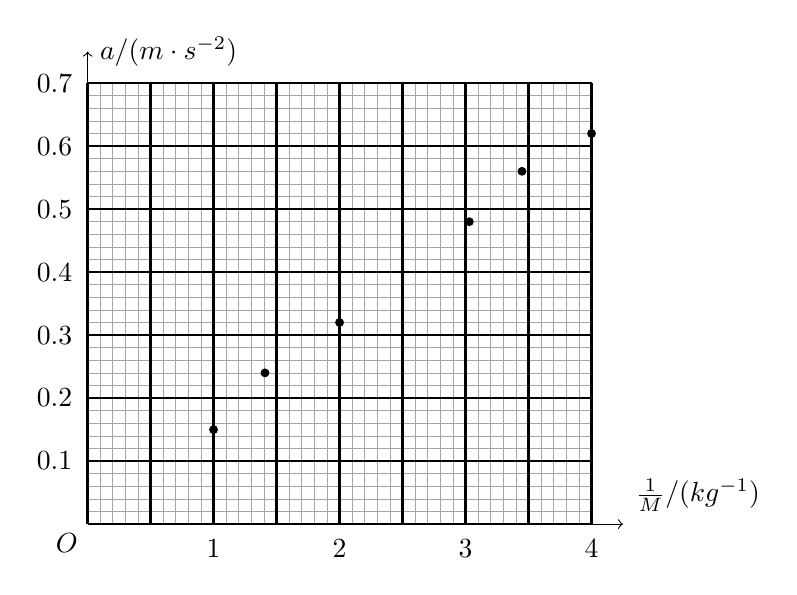
\begin{tikzpicture}[scale=0.8]

\draw[gray!70,very thin,step=0.2] (0,0) grid (8,7);
\draw[thick] (0,0) grid (8,7);
\draw [->] (0,0) node [below left]{$ O $}--(8.5,0) node[above right=1pt] {$ \frac{1}{M}/(kg^{-1}) $} ;
\draw [->] (0,0)--(0,7.5) node[right=1pt] {$ a/(m \cdot s^{-2}) $} ;


\draw (2,0) node[below=2pt] {$ 1 $};
\draw (4,0) node[below=2pt] {$ 2 $};
\draw (6,0) node[below=2pt] {$ 3 $};
\draw (8,0) node[below=2pt] {$ 4 $};


\foreach \x in {1,...,7}
{
\draw (0,\x) node[left=2pt] {$ 0.\x $};	
}



\fill (8,6.2) circle [radius=2pt];
\fill (6.8965,5.6) circle [radius=2pt];
\fill (6.06,4.8) circle [radius=2pt];
\fill (4,3.2) circle [radius=2pt];
\fill (2.816,2.4) circle [radius=2pt];
\fill (2,1.5) circle [radius=2pt];

\end{tikzpicture}
\caption{}\label{2020:北京15:2}
\end{figure}




\item 
在探究加速度与力的关系实验之前,需要思考如何测“力”。请在图 \ref{2020:北京15:3} 中画出小车受力的示意图。为了简
化“力”的测量,下列说法正确的是: \underlinegap (选填选项前的字母)
。
\begin{figure}[h!]
\centering
\includesvg[width=0.22\linewidth]{picture/svg/GZ-3-tiyou-0796}
\caption{}\label{2020:北京15:3}
\end{figure}

\fourchoices
{使小车沿倾角合适的斜面运动,小车受力可等效为只受绳的拉力}
{若斜面倾角过大,小车所受合力将小于绳的拉力}
{无论小车运动的加速度多大,砂和桶的重力都等于绳的拉力}
{让小车的运动趋近于匀速运动,砂和桶的重力才近似等于绳的拉力}

\end{enumerate}


\tk{
\begin{enumerate}
\item
B	
\item 	
如图所示
\begin{center}
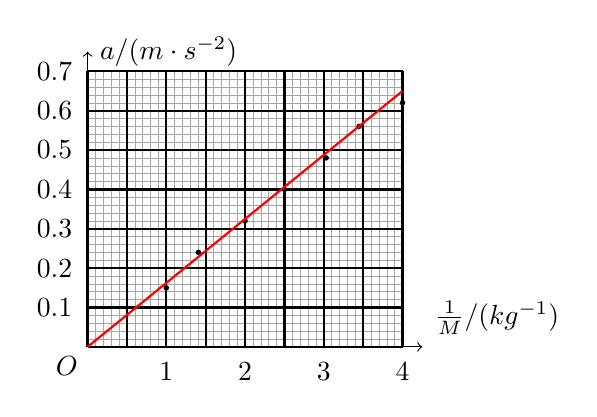
\begin{tikzpicture}[scale=0.5]
\draw[gray!70,very thin,step=0.2] (0,0) grid (8,7);
\draw[thick] (0,0) grid (8,7);
\draw [->] (0,0) node [below left]{$ O $}--(8.5,0) node[above right=1pt] {$ \frac{1}{M}/(kg^{-1}) $} ;
\draw [->] (0,0)--(0,7.5) node[right=1pt] {$ a/(m \cdot s^{-2}) $} ;


\draw (2,0) node[below=2pt] {$ 1 $};
\draw (4,0) node[below=2pt] {$ 2 $};
\draw (6,0) node[below=2pt] {$ 3 $};
\draw (8,0) node[below=2pt] {$ 4 $};


\foreach \x in {1,...,7}
{
\draw (0,\x) node[left=2pt] {$ 0.\x $};	
}



\fill (8,6.2) circle [radius=2pt];
\fill (6.8965,5.6) circle [radius=2pt];
\fill (6.06,4.8) circle [radius=2pt];
\fill (4,3.2) circle [radius=2pt];
\fill (2.816,2.4) circle [radius=2pt];
\fill (2,1.5) circle [radius=2pt];
\fill (5,4) circle [radius=2pt];
\draw[red,thick] (0,0) -- (8,6.5);
\end{tikzpicture}
\end{center}
\item 	
AD
\end{enumerate}
} 


\item 
用图 \ref{2020:北京16:1} 所示的 \subref{2020:北京16:1a} 、 \subref{2020:北京16:1b} 两种方法测量某电源的电动势和内电阻(约为 $ 1 \ \Omega $)
。其中 $ R $ 为电阻箱,电流表的内电阻约
为 $ 0.1 \ \Omega $,电压表的内电阻约为 $ 3 \ k\Omega $。
\begin{figure}[h!]
\centering
\begin{subfigure}{0.4\linewidth}
\centering
\includesvg[width=0.8\linewidth]{picture/svg/GZ-3-tiyou-0797} 
\caption{}\label{2020:北京16:1a}
\end{subfigure}
\hfil
\begin{subfigure}{0.4\linewidth}
\centering
\includesvg[width=0.8\linewidth]{picture/svg/GZ-3-tiyou-0798} 
\caption{}\label{2020:北京16:1b}
\end{subfigure}
\caption{}\label{2020:北京16:1}
\end{figure}

\begin{enumerate}
\item
利用图 \ref{2020:北京16:1} 中 \subref{2020:北京16:1a} 图实验电路测电源的电动势 $ E $ 和内电阻 $ r $,所测量的实际是图 \ref{2020:北京16:2} 中虚线框所示“等效电源”
的电动势 $ E ^{\prime} $ 和内电阻 $ r ^{\prime} $ 。若电流表内电阻用 $ R_{A} $ 表示,请你用 $ E $、$ r $ 和 $ R_{A} $ 表示出 $ E ^{\prime} $ 、 $ r ^{\prime} $ ,并简要说明理
由。
\begin{figure}[h!]
\centering
\includesvg[width=0.33\linewidth]{picture/svg/GZ-3-tiyou-0799}
\caption{}\label{2020:北京16:2}
\end{figure}



\item 
某同学利用图像分析甲、乙两种方法中由电表内电阻引起的实验误差。在图 \ref{2020:北京16:3} 中,实线是根据实验数据
(图 \subref{2020:北京16:1a} :$ U=IR $,图 \subref{2020:北京16:1b} :$\left.I=\frac{U}{R}\right)$)描点作图得到的 $ U-I $ 图像;虚线是该电源的路端电压 $ U $ 随电流 $ I $ 变化的
$ U-I $ 图像(没有电表内电阻影响的理想情况)。
\begin{figure}[h!]
\centering
\includesvg[width=0.75\linewidth]{picture/svg/GZ-3-tiyou-0800}
\caption{}\label{2020:北京16:3}
\end{figure}




在图 \ref{2020:北京16:3} 中,对应图 \subref{2020:北京16:1a} 电路分析的 $ U-I $ 图像是: \underlinegap ;对应图 \subref{2020:北京16:1b} 电路分析的 $ U-I $ 图像是: \underlinegap 。
\item 
综合上述分析,为了减小由电表内电阻引起的实验误差,本实验应选择图 \ref{2020:北京16:1} 中的 \underlinegap (填“\subref{2020:北京16:1a}”或“\subref{2020:北京16:1b}”)
。

\end{enumerate}


\tk{
\begin{enumerate}
\item
$E^{\prime}=E $,$ r ^{\prime} =r+R_{\mathrm{A}} $。理由如下:\\
将电源和电流表视为等效电源,电源电动势是电源本身具有的属性,电流表不具有产生电动
势的本领,所以等效电源的电动势仍然为
$E^{\prime}=E $,
而电流表的内阻和电动势的内阻作为等效电源的内阻,即$ r ^{\prime} =r+R_{\mathrm{A}} $。
\item 
C \quad A
\item 
\subref{2020:北京16:1b}
\end{enumerate}
} 


\gaokaojs

\item
无人机在距离水平地面高度 $ h $ 处,以速度 $ v_{0} $ 水平匀速飞行并释放一包裹,不计空气阻力,重力加速度为 $ g $。
\begin{enumerate}
\item
求包裹释放点到落地点的水平距离 $ x $;
\item 
求包裹落地时的速度大小 $ v $;
\item 
以释放点为坐标原点,初速度方向为 $ x $ 轴方向,竖直向下为 $ y $ 轴方向,建立平面直角坐标系,写出该包
裹运动的轨迹方程。
\end{enumerate}




\banswer{
\begin{enumerate}
\item
$x=v_{0} \sqrt{\frac{2 h}{g}}$
\item 
$v=\sqrt{v_{0}^{2}+2 g h}$
\item 
$y=\frac{g}{2 v_{0}^{2}} x^{2}$
\end{enumerate}
}


\vfill

\item
如图 \subref{2020:北京18:a} 所示, $ N =200 $ 匝的线圈(图中只画了 $ 2 $ 匝),电阻 $ r=2 \ \Omega $ ,其两端与一个 $ R = 48 \ \Omega $ 的电阻相连,线
圈内有指向纸内方向的磁场。线圈中的磁通量按图 \subref{2020:北京18:b} 所示规律变化。
\begin{enumerate}
\item
判断通过电阻 $ R $ 的电流方向;
\item 
求线圈产生的感应电动势 $ E $;
\item 
求电阻 $ R $ 两端的电压 $ U $。
\end{enumerate}
\begin{figure}[h!]
\flushright
\begin{subfigure}{0.3\linewidth}
\centering
\includesvg[width=0.87\linewidth]{picture/svg/GZ-3-tiyou-0805} 
\caption{}\label{2020:北京18:a}
\end{subfigure}
\begin{subfigure}{0.3\linewidth}
\centering
\includesvg[width=0.87\linewidth]{picture/svg/GZ-3-tiyou-0806} 
\caption{}\label{2020:北京18:b}
\end{subfigure}
\end{figure}


\banswer{
\begin{enumerate}
\item
$a \rightarrow b$
\item 
$ E=10 \ V $
\item 
$ U=9.6 \ V $
\end{enumerate}
}




\newpage
\item 
如图 \subref{2020:北京19:a} 所示,真空中有一长直细金属导线 $ MN $,与导线同轴放置一半径为 $ R $ 的金属圆柱面。假设导线沿径向均
匀射出速率相同的电子,已知电子质量为 $ m $,电荷量为 $ e $。不考虑出射电子间的相互作用。
\begin{enumerate}
\item
可以用以下两种实验方案测量出射电子的初速度:
\begin{enumerate}
\item
在柱面和导线之间,只加恒定电压;

\item 
在柱面内,只加与 $ MN $ 平行的匀强磁场。
\end{enumerate}


当电压为 $ U_{0} $ 或磁感应强度为 $ B_{0} $ 时,刚好没有电子到达柱面。分别计算出射电子的初速度 $ v_{0} $。

\item 
撤去柱面,沿柱面原位置放置一个弧长为 $ a $、长度为 $ b $ 的金属片,如图 \subref{2020:北京19:b} 所示。在该金属片上检测到出
射电子形成的电流为 $ I $ ,电子流对该金属片的压强为 $ p $。求单位长度导线单位时间内出射电子的总动能。

\end{enumerate}
\begin{figure}[h!]
\flushright
\begin{subfigure}{0.3\linewidth}
\centering
\includesvg[width=0.5\linewidth]{picture/svg/GZ-3-tiyou-0807} 
\caption{}\label{2020:北京19:a}
\end{subfigure}
\begin{subfigure}{0.3\linewidth}
\centering
\includesvg[width=0.5\linewidth]{picture/svg/GZ-3-tiyou-0808} 
\caption{}\label{2020:北京19:b}
\end{subfigure}
\end{figure}


\banswer{
\begin{enumerate}
\item
\begin{enumerate}
\item
当电压为$ U_{0} $时$v_{0}=\sqrt{\frac{2 e U_{0}}{m}}$
\item 
磁感应强度为$ B_{0} $时$v_{0}=\frac{B_{0} q R}{2 m}$(粒子的运动轨迹在水平面内)
\end{enumerate}
\item 
$\frac{e \pi ab p^{2} R}{m I}$
\end{enumerate}
}



\newpage
\item 
某试验列车按照设定的直线运动模式,利用计算机控制制动装置,实现安全准确地进站停车。制动装置包括电
气制动和机械制动两部分。图 \subref{2020:北京20:a} 所示为该列车在进站停车过程中设定的加速度大小 $ a $车 随速度 $ v $ 的变化曲线。
\begin{enumerate}
\item
求列车速度从 $ 20 \ m/s $ 降至 $ 3 \ m/s $ 经过的时间 $ t $ 及行进的距离 $ x $。
\item 
有关列车电气制动,可以借助图 \subref{2020:北京20:b} 模型来理解。图中水平平行金属导轨处于竖直方向的匀强磁场中,回
路中的电阻阻值为 $ R $,不计金属棒 $ MN $ 及导轨的电阻。 $ MN $ 沿导轨向右运动的过程,对应列车的电气制
动过程,可假设 $ MN $ 棒运动的速度与列车的速度、棒的加速度与列车电气制动产生的加速度成正比。列
车开始制动时,其速度和电气制动产生的加速度大小对应图 $ 1 $ 中的 $ P $ 点。论证电气制动产生的加速度大
小随列车速度变化的关系,并在图 \subref{2020:北京20:a}中画出图线。

\item 
制动过程中,除机械制动和电气制动外,列车还会受到随车速减小而减小的空气阻力。分析说明列车从$ 100 \ m/s $ 减到 $ 3 \ m/s $ 的过程中,在哪个速度附近所需机械制动最强?


\end{enumerate}
\begin{figure}[h!]
\flushright 
\begin{subfigure}{0.45\linewidth}
\centering
\includesvg[width=0.97\linewidth]{picture/svg/GZ-3-tiyou-0809}
\caption{}\label{2020:北京20:a}
\end{subfigure}
\begin{subfigure}{0.4\linewidth}
\centering
\includesvg[width=0.95\linewidth]{picture/svg/GZ-3-tiyou-0810} 
\caption{}\label{2020:北京20:b}
\end{subfigure}
\end{figure}

\banswer{
\begin{enumerate}
\item
$t=\frac{170}{7} = \approx 24.3 \ s $\\
$ x = \frac{1955}{7} = \approx 279.3 \ m$
\item 
列车电气制动产生的加速度与列车的速度成正比,为过$ P $ 点的
正比例函数,论证过程略。画出的图线如下图所示:
\begin{center}
\includesvg[width=0.93\linewidth]{picture/svg/GZ-3-tiyou-0813} 
\end{center}
\item 
由于空气阻力造成的加速度和电气制动造成的加速度之和依然与速度成正比关系,易知在$ 3 \ m/s $附近所需的机械制动最强。
\end{enumerate}
}



\end{enumerate}

%
\gaokaoheader{2020}{上海卷}





\gaokaoxz


\begin{enumerate}
\item
原子核符号 $^{17}_{8} O $ 中,$ 17 $表示 \xzanswer{D} 
\fourchoices
{电子数}
{质子数}
{中子数}
{核子数}



\item
下列电磁波中穿透能力最强的是 \xzanswer{A} 
\fourchoices
{$ \gamma $射线}
{$ X $射线}
{紫外线}
{红外线}


\item 
天然放射性元素的发现揭示了 \xzanswer{D} 
\fourchoices
{质子拥有复杂结构}
{分子拥有复杂结构}
{原子拥有复杂结构}
{原子核拥有复杂结构}



\item
下列不是基本单位的是 \xzanswer{A} 
\fourchoices
{牛顿}
{千克}
{米}
{秒}


\item 
太阳辐射的能量主要来自于太阳内部的 \xzanswer{D}

\fourchoices
{化学反应}
{裂变反应}
{链式反应}
{热核反应}




\item
一个带电粒子的电量可能为 \xzanswer{A}
\fourchoices
{$2 e$}
{$1.6 e$}
{$1.9 \times 10^{-16} e$}
{$1.6 \times 10^{-19} e$}







\item 
机械波在一个周期内传播的距离等于 \xzanswer{A} 
\fourchoices
{一个波长}
{四个波长}
{一个振幅}
{四个振幅}



\item
下列物理量中是矢量的为 \xzanswer{B} 
\fourchoices
{磁通量}
{磁感应强度}
{电流强度}
{磁通量密度}


\item 
如图将小车沿光滑斜面释放瞬间,小车的 \xzanswer{A} 
\begin{figure}[h!]
\centering
\includesvg[width=0.19\linewidth]{picture/svg/GZ-3-tiyou-1653}
\end{figure}

\fourchoices
{速度为$ 0 $}
{动能不为$ 0 $}
{加速度为$ 0 $}
{合外力为$ 0 $}



\item
如图,质量为$ M $、内壁光滑的气缸开口向下悬挂于天花板。横截面积为$ S $、质量为$ m $的活塞将一定质量的气体封闭在气缸内。平衡后,封闭气体的压强为(大气压强为$ p_{0} $) \xzanswer{C} 
\begin{figure}[h!]
\centering
\includesvg[width=0.2\linewidth]{picture/svg/GZ-3-tiyou-1654}
\end{figure}


\fourchoices
{$p_{0}-\frac{M g}{S}$}
{$p_{0}+\frac{M g}{S}$}
{$p_{0}-\frac{m g}{S}$}
{$p_{0}+\frac{m g}{S}$}



\item
如图,陀螺在平铺于水平桌面的白纸上稳定转动,若在陀螺表面滴上几滴墨水,则由于陀螺转动甩出的墨水在纸上的痕迹最接近于 \xzanswer{B} 
\begin{figure}[h!]
\centering
\includesvg[width=0.19\linewidth]{picture/svg/GZ-3-tiyou-1655}
\end{figure}

\pfourchoices
{\includesvg[width=3cm]{picture/svg/GZ-3-tiyou-1657}}
{\includesvg[width=3cm]{picture/svg/GZ-3-tiyou-1658}}
{\includesvg[width=3cm]{picture/svg/GZ-3-tiyou-1659}}
{\includesvg[width=3cm]{picture/svg/GZ-3-tiyou-1660}}






\item
小车从一斜面下滑,受到恒定阻力,下列$ v-t $图中哪个能正确反应小车的运动情况? \xzanswer{C} 

\pfourchoices
{\includesvg[width=3cm]{picture/svg/GZ-3-tiyou-1661}}
{\includesvg[width=3cm]{picture/svg/GZ-3-tiyou-1662}}
{\includesvg[width=3cm]{picture/svg/GZ-3-tiyou-1663}}
{\includesvg[width=3cm]{picture/svg/GZ-3-tiyou-1664}}




\item
如图,在上端有活塞的玻璃管底部放置一小块硝化棉,用手快速向下压活塞,可观察到硝化棉被点燃,在此过程中 \xzanswer{B} 
\begin{figure}[h!]
\centering
\includesvg[width=0.036\linewidth]{picture/svg/GZ-3-tiyou-1665}
\end{figure}

\fourchoices
{气体对外界做功,气体内能增加}
{外界对气体做功,气体内能增加}
{气体对外界做功,气体内能减少}
{外界对气体做功,气体内能减少}




\item
波速$ v=4 \ m /s $,沿$ x $轴传播的横波,某时刻质点$ a $沿$ y $轴正方向运动,则波的传播方向与频率分别为 \xzanswer{D} 
\begin{figure}[h!]
\centering
\includesvg[width=0.33\linewidth]{picture/svg/GZ-3-tiyou-1666}
\end{figure}

\fourchoices
{$ x $轴正方向,$ 2 \ Hz $}
{$ x $轴正方向,$ 0.5 \ Hz $}
{$ x $轴负方向,$ 2 \ Hz $}
{$ x $轴负方向,$ 0.5 \ Hz $}





\item
如图,在负点电荷$ a $的电场中,$ M $、$ N $两点与$ a $所在处共线,两点的电场强度大小分别为$ E_M $和$ E_N $,则它们的电场强度 \xzanswer{B} 
\begin{figure}[h!]
\centering
\includesvg[width=0.5\linewidth]{picture/svg/GZ-3-tiyou-1667}
\end{figure}


\fourchoices
{方向相同, $E_{M}>E_{N}$}
{方向相反, $E_{M}>E_{N}$}
{方向相同, $E_{M}<E_{N}$}
{方向相反,$E_{M}<E_{N}$}





\item
质量为$ 2.0 \times 10^{5} \ kg $的火箭,发射时受到竖直向上、大小为$ 6.0 \times 10^{6} \ N $的推力,加速度大小为(不要忽略重力,$ g=10 \ m/s^{2} $) \xzanswer{C} 
\fourchoices
{$ 4.0 \ m/s^{2} $}
{$ 12 \ m/s^{2} $}
{$ 20 \ m/s^{2} $}
{$ 30 \ m/s^{2} $}




\item
阻值分别为$ 2 \ \Omega $、$ 4 \ \Omega $、$ 8 \ \Omega $的三个电阻$ R_{1} $,$ R_{2} $,$ R_{3} $如图所示连接,电路中$ ab $两点间电压恒定,当$ R_{1} $功率为$ 2 \ W $时,$ R_{3} $的功率为 \xzanswer{A} 
\begin{figure}[h!]
\centering
\includesvg[width=0.38\linewidth]{picture/svg/GZ-3-tiyou-1668}
\end{figure}

\fourchoices
{$ 0.5 \ W $}
{$ 1 \ W $}
{$ 4 \ W $}
{$ 8 \ W $}




\item
已知有三个力可以达成力的平衡,以下哪组是不可能的 \xzanswer{C} 

\fourchoices
{$ 4 \ N $,$ 7 \ N $,$ 8 \ N $}
{$ 1 \ N $,$ 8 \ N $,$ 8 \ N $}
{$ 1 \ N $,$ 4 \ N $,$ 6 \ N $}
{$ 1 \ N $,$ 4 \ N $,$ 5 \ N $}



\item 
列车沿平直轨道匀速行驶,车厢光滑地板上有一个相对列车静止的物体,当列车刹车过程中,物体相对轨道 \xzanswer{A} 

\fourchoices
{向前匀速运动}
{向后匀速运动}
{向前加速运动}
{向后加速运动}



\item 
如图,螺线管与电流表组成闭合回路,不能使电流表指针偏转的是(忽略地磁影响) \xzanswer{D} 
\begin{figure}[h!]
\centering
\includesvg[width=0.23\linewidth]{picture/svg/GZ-3-tiyou-1669}
\end{figure}

\fourchoices
{螺线管不动,磁铁向上运动}
{螺线管不动,磁铁向左运动}
{磁铁不动,螺线管向上运动}
{磁铁与螺线管以相同速度一起运动}





\item
洗衣机脱水桶上螺丝旋转半径为$ 0.2 \ m $,转速为$ 1200 \ r/min $,小螺丝转动周期和线速度大小分别为 \xzanswer{A} 

\fourchoices
{$ 0.05 \ s $,$ 8 \pi m/s $}
{$ 20 \ s $,$ 8 \pi m/s $}
{$ 0.05 \ s $,$ 16 \pi m/s $}
{$ 20 \ s $,$ 16 \pi m/s $}



\item
如图,质量为$ m $的小球,自井台上方$ H $高处,由静止释放。井深为$ h $,以井台为零势能面,小球落至井底时的的机械能为(不计阻力) \xzanswer{C} 
\begin{figure}[h!]
\centering
\includesvg[width=0.23\linewidth]{picture/svg/GZ-3-tiyou-1670}
\end{figure}

\fourchoices
{$ mgh $}
{$ mg ( H-h $) }
{$ mgH $}
{$ mg ( H+h) $}




\item
电动机以$ v $,竖直匀速提升质量为$ m $的物体时,测得电动机两端电压为$ U $,通过电动机的电流为$ I $,则电动机的效率为 \xzanswer{D} 


\fourchoices
{$\frac{U I}{m g v}$}
{$\frac{U I}{m g}$}
{$\frac{m g}{U I}$}
{$\frac{m g v}{U I}$}




\item
在磁场强度为$ B $的匀强磁场中,通过面积为$ S $的矩形面的磁通量大小不可能是 \xzanswer{D} 

\fourchoices
{$ 0 $}
{$ BS $}
{$ 0.5BS $}
{$ 2BS $}





\item
一物体在地面附近以小于$ g $的加速度沿竖直方向匀加速下降,运动过程中物体 \xzanswer{C} 

\fourchoices
{动能增大,机械能增大}
{动能减小,机械能增大}
{动能增大,机械能减小}
{动能减小,机械能减小}




\item
在匀强磁场中,长为$ 10 \ cm $的直导线与磁场方向垂直。当其通有$ 10 \ A $电流时,受到的磁场力大小为$ 0.2 \ N $,则该磁场的磁感应强度大小为 \xzanswer{C} 

\fourchoices
{$ 0.01 \ T $}
{$ 0.02 \ T $}
{$ 0.2 \ T $}
{$ 5 \ T $}




\item
地球在公转轨道的近日点和远日点的加速度 \xzanswer{D} 

\fourchoices
{大小相同,方向相同}
{大小不同,方向相同}
{大小相同,方向不同}
{大小不同,方向不同}




\item
质量为$ 0.1 \ kg $的小球做自由落体运动,下落前$ 2 \ s $内重力的平均功率和$ 2 \ s $末重力的瞬时功率分别为 \xzanswer{B} 

\fourchoices
{$ 10 \ W $,$ 10 \ W $}
{$ 10 \ W $,$ 20 \ W $}
{$ 20 \ W $,$ 10 \ W $}
{$ 20 \ W $,$ 20 \ W $}



\item
如图,$ O $为平衡位置,小球在$ B $、$ C $间做无摩擦往复运动。由$ B $向$ O $运动的过程中,振子的 \xzanswer{C} 
\begin{figure}[h!]
\centering
\includesvg[width=0.25\linewidth]{picture/svg/GZ-3-tiyou-1671}
\end{figure}

\fourchoices
{动能增大,势能增大}
{动能减小,势能增大}
{动能增大,势能减小}
{动能减小,势能减小}


\item 
下列选项中,能正确描述某种气体分子速率分布规律的是 \xzanswer{A} 

\pfourchoices
{\includesvg[width=4.3cm]{picture/svg/GZ-3-tiyou-1672}}
{\includesvg[width=4.3cm]{picture/svg/GZ-3-tiyou-1673}}
{\includesvg[width=4.3cm]{picture/svg/GZ-3-tiyou-1674}}
{\includesvg[width=4.3cm]{picture/svg/GZ-3-tiyou-1675}}




\item
如图,两通电直导线$ a $、$ b $平行,$ b $电流向上。两导线相互吸引,则$ a $电流在$ b $处产生的磁场方向 \xzanswer{B} 
\begin{figure}[h!]
\centering
\includesvg[width=0.13\linewidth]{picture/svg/GZ-3-tiyou-1676}
\end{figure}

\fourchoices
{向左}
{垂直纸面向里}
{向右}
{垂直纸面向外}






\item
棒$ ab $在匀强磁场中沿导轨运动时,棒中感应电流方向如图。则$ ab $棒的运动方向和螺线管内部磁场方向分别为 \xzanswer{C} 
\begin{figure}[h!]
\centering
\includesvg[width=0.23\linewidth]{picture/svg/GZ-3-tiyou-1677}
\end{figure}

\fourchoices
{向左,$ M $指向$ N $}
{向右,$ M $指向$ N $}
{向左,$ N $}
{向右,$ N $指向$ M $}



\item 
如图所示,电压$ U $恒定,灯泡$ A $、$ B $阻值不变,若滑动变阻器$ R $的滑片右移,则 \xzanswer{B} 
\begin{figure}[h!]
\centering
\includesvg[width=0.23\linewidth]{picture/svg/GZ-3-tiyou-1678}
\end{figure}

\fourchoices
{$ A $灯变亮,$ B $灯变亮}
{$ A $灯变暗,$ B $灯变亮}
{$ A $灯变亮,$ B $灯变暗}
{$ A $灯变暗,$ B $灯变暗}



\item
如图,质量为$ m $的物体静置于地面。用手缓慢提拉与物体相连的弹簧上端,使物体升高$ h $,手做功一定 \xzanswer{B} 
\begin{figure}[h!]
\centering
\includesvg[width=0.14\linewidth]{picture/svg/GZ-3-tiyou-1679}
\end{figure}

\fourchoices
{等于$ mgh $}
{大于$ mgh $}
{小于$ mgh $}
{大于$ 2 \ m gh $}




\item
固定三通管,$ AB $管竖直,$ CD $管水平,水银在管子的$ A $端封闭了一定量的气体。打开阀门,则$ A $端气体 \xzanswer{B} 
\begin{figure}[h!]
\centering
\includesvg[width=0.15\linewidth]{picture/svg/GZ-3-tiyou-1680}
\end{figure}

\fourchoices
{体积、压强均增大}
{体积减小,压强增大}
{体积、压强均减小}
{体积增大,压强减小}




\gaokaosy




\item
\begin{enumerate}
\item
在“用$ DIS $研究机械能守恒定律”的实验中,摆锤释放器的作用是保证每次释放摆锤
时,摆锤的位置 \underlinegap 和速度 \underlinegap 。


\tk{相同 \quad 为零} 

\item 
在“用$ DIS $研究温度不变时,一定质量的气体与体积的关系”的实验中,
压强传感器 \underlinegap (选填“需要”或“不需要”)调零。能描述缓慢压缩气体过程中,气体压强$ p $与$ V $间关系的图线
是 \underlinegap 。(选填“ \subref{2020上海36a} ”或“ \subref{2020上海36b} ”)
\begin{figure}[h!]
\centering
\begin{subfigure}{0.4\linewidth}
\centering
\includesvg[width=0.5\linewidth]{picture/svg/GZ-3-tiyou-1681} 
\caption{}\label{2020上海36a}
\end{subfigure}
\begin{subfigure}{0.4\linewidth}
\centering
\includesvg[width=0.5\linewidth]{picture/svg/GZ-3-tiyou-1682} 
\caption{}\label{2020上海36b}
\end{subfigure}
\end{figure}
\end{enumerate}



\tk{不需要 \quad \subref{2020上海36a} } 



\item 
在“用$ DIS $研究通电螺线管的磁感应强度”的实验中,磁传感器 \underlinegap (选填“需要”或“不需要”)调零。能描述通电螺线管内磁感应强度大小$ B $与磁传感器插入螺线管的长度$ x $间关系的图线可能是 \underlinegap 。(选填“ \subref{2020上海37a} ”或者“ \subref{2020上海37b} ”
)
\begin{figure}[h!]
\centering
\begin{subfigure}{0.4\linewidth}
\centering
\includesvg[width=0.7\linewidth]{picture/svg/GZ-3-tiyou-1683} 
\caption{}\label{2020上海37a}
\end{subfigure}
\begin{subfigure}{0.4\linewidth}
\centering
\includesvg[width=0.7\linewidth]{picture/svg/GZ-3-tiyou-1684} 
\caption{}\label{2020上海37b}
\end{subfigure}
\end{figure}


\tk{需要 \quad \subref{2020上海37b} } 




\newpage


\gaokaojs




\item 
如图,在点电荷电场中,从$ A $点由静止释放一带负电的微粒,仅受电场力的作用,微粒
\begin{enumerate}
\item
向何方向运动?
\item 
加速度大小如何变化?
\end{enumerate}
\begin{figure}[h!]
\flushright 
\includesvg[width=0.2\linewidth]{picture/svg/GZ-3-tiyou-1685}
\end{figure}

\banswer{
\begin{enumerate}
\item
向左
\item 
变大
\end{enumerate}
}



\item 
如图,长为$ 10 \ m $的光滑斜面倾角为$ 30 \degree $。质量为$ m $的物体在一沿斜面向上、大小为$ mg $的拉力作用下,由斜面底端由静止开始沿斜面向上运动。($ g $取$ 10 \ m/s^{2} $)
\begin{enumerate}
\item
求出物体运动到斜面顶端时的速度大小;
\item 
取斜面底端为零势能面,通过分析说明物体沿斜面运动过程中动能与重力势能的大小
关系。

\end{enumerate}
\begin{figure}[h!]
\flushright
\includesvg[width=0.22\linewidth]{picture/svg/GZ-3-tiyou-1686}
\end{figure}


\banswer{
\begin{enumerate}
\item
$ 10\ m/s $
\item 
$E_{k}=E_{p}$
\end{enumerate}
}



\end{enumerate}


%
\gaokaoheader{2020}{海南卷}





\gaokaoxz


\begin{enumerate}
	%\renewcommand{\labelenumi}{\arabic{enumi}.}
	% A(\Alph) a(\alph) I(\Roman) i(\roman) 1(\arabic)
	%设定全局标号series=example	%引用全局变量resume=example
	%[topsep=-0.3em,parsep=-0.3em,itemsep=-0.3em,partopsep=-0.3em]
	%可使用leftmargin调整列表环境左边的空白长度 [leftmargin=0em]
	\item
	$ 100 $年前,卢瑟福猜想在原子核内除质子外还存在着另一种粒子$ X $,后来科学家用$ \alpha $粒子轰击铍核证实了这一猜想,该核反应方程为:${ }_{2}^{4} He+{ }_{4}^{9} Be \rightarrow{ }_{6}^{12} C+{ }_{n}^{m} X$,则 \xzanswer{A}

 

\fourchoices
{$m=1, \quad n=0, \quad X$ 是中子}
{$m=1, \quad n=0, \quad X$ 是电子}
{$m=0, \quad n=1, \quad X$ 是中子}
{$m=0, \quad n=1, \quad X$ 是电子}



\item
如图,上网课时小明把手机放在斜面上,手机处于静止状态。则斜面对手机的 \xzanswer{B} 
% TODO: \usepackage{graphicx} required
\begin{figure}[h!]
	\centering
	\includegraphics[width=0.18\linewidth]{picture/screenshot092}
\end{figure}

\fourchoices
{支持力竖直向上}
{支持力小于手机所受的重力}
{摩擦力沿斜面向下}
{摩擦力大于手机所受的重力沿斜面向下的分力}



\item
图 \subref{2020海南3a} 、 \subref{2020海南3b} 分别表示两种电流的波形,其中图 \subref{2020海南3b} 所示电流按正弦规律变化,分别用$ I_{1} $和$ I_{2} $表示 \subref{2020海南3a} 和 \subref{2020海南3b} 两电流的有效值,则 \xzanswer{D} 
\begin{figure}[h!]
	\centering
	\begin{subfigure}{0.4\linewidth}
		\centering
		\includesvg[width=0.6\linewidth]{picture/svg/GZ-3-tiyou-1687} 
		\caption{}\label{2020海南3a}
	\end{subfigure}
	\begin{subfigure}{0.4\linewidth}
		\centering
		\includesvg[width=0.6\linewidth]{picture/svg/GZ-3-tiyou-1688} 
		\caption{}\label{2020海南3b}
	\end{subfigure}
\end{figure}


\fourchoices
{$I_{1}: I_{2}=2: 1$}
{$I_{1}: I_{2}=1: 2$}
{$I_{1}: I_{2}=1: \sqrt{2}$}
{$I_{1}: I_{2}=\sqrt{2}: 1$}





\item
 一车载加热器(额定电压为 $24 \ V$ )发热部分的电路如图所示, $a$ 、$ b $、$ c $ 是三个接线
端点, 设$ ab $、$ ac $、$ bc $ 间的功率分别为 $P_{ab} $、$ P_{ac} $、$ P_{bc} $, 则 \xzanswer{D} 
\begin{figure}[h!]
	\centering
	\includesvg[width=0.23\linewidth]{picture/svg/GZ-3-tiyou-1689}
\end{figure}


\fourchoices
{$P_{ab}>P_{bc}$}
{$ P_{a b}=P_{a c}$}
{$P_{ac}=P_{b c}$}
{$P_{ab}<P_{ac}$}



\item
下列说法正确的是 \xzanswer{A} 

\fourchoices
{单色光在介质中传播时,介质的折射率越大,光的传播速度越小}
{观察者靠近声波波源的过程中,接收到的声波频率小于波源频率}
{同一个双缝干涉实验中,蓝光产生的干涉条纹间距比红光的大}
{两束频率不同的光,可以产生干涉现象}





\item
如图,在一个蹄形电磁铁的两个磁极的正中间放置一根长直导线,当导线中通有垂直于纸面向里的电流$ I $时,导线所受安培力的方向为 \xzanswer{B} 
\begin{figure}[h!]
	\centering
	\includesvg[width=0.18\linewidth]{picture/svg/GZ-3-tiyou-1690}
\end{figure}

\fourchoices
{向上}
{向下}
{向左}
{向右}



\item
$ 2020 $年$ 5 $月$ 5 $日,长征五号$ B $运载火箭在中国文昌航天发射场成功首飞,将新一代载人飞船试验船送入太空,若试验船绕地球做匀速圆周运动,周期为$ T $,离地高度为$ h $,已知地球半径为$ R $,万有引力常量为$ G $,则 \xzanswer{B} 

\fourchoices
{试验船的运行速度为 $\frac{2 \pi R}{T}$}
{地球的第一宇宙速度为 $\frac{2 \pi}{T} \sqrt{\frac{(R+h)^{3}}{R}}$}
{地球的质量为 $\frac{2 \pi(R+h)^{3}}{G T^{2}}$}
{地球表面的重力加速度为 $\frac{4 \pi^{2}(R+h)^{2}}{R T^{2}}$}

\item 
太空探测器常装配离子发动机,其基本原理是将被电离的原子从发动机尾部高速喷出,从而为探测器提供推力,若某探测器质量为$ 490 \ kg $,离子以$ 30 \ km /s $的速率(远大于探测器的飞行速率)向后喷出,流量为$ 3.0 \times 10^{-3} \ g /s $,则探测器获得的平均推力大小为 \xzanswer{C} 

\fourchoices
{$ 1.47 \ N $}
{$ 0.147 \ N $}
{$ 0.09 \ N $}
{$0.009 \ N $}



\item
一列简谐横波沿$ x $轴正方向传播,波的周期为$ 0.2 \ s $,某时刻的波形如图所示.则 \xzanswer{AC} 
\begin{figure}[h!]
	\centering
	\includesvg[width=0.25\linewidth]{picture/svg/GZ-3-tiyou-1691}
\end{figure}

\fourchoices
{该波的波长为$ 8 \ m $}
{该波的波速为$ 50 \ m /s $}
{该时刻质点$ P $向$ y $轴负方向运动}
{该时刻质点$ Q $向$ y $轴负方向运动}


\item 
空间存在如图所示的静电场,$ a $、$ b $、$ c $、$ d $为电场中的四个点,则 \xzanswer{AD} 
\begin{figure}[h!]
	\centering
	\includesvg[width=0.23\linewidth]{picture/svg/GZ-3-tiyou-1692}
\end{figure}

\fourchoices
{$ a $点的场强比$ b $点的大}
{$ d $点的电势比$ c $点的低}
{质子在$ d $点的电势能比在$ c $点的小}
{将电子从$ a $点移动到$ b $点,电场力做正功}




\item
小朋友玩水枪游戏时,若水从枪口沿水平方向射出的速度大小为$ 10 \ m /s $,水射出后落到水平地面上。已知枪口离地高度为$ 1.25 \ m $,$ g=10 \ m /s^{2} $,忽略空气阻力,则射出的水 \xzanswer{BD} 

\fourchoices
{在空中的运动时间为$ 0.25 \ s $}
{水平射程为$ 5 \ m $}
{落地时的速度大小为$ 15 \ m /s $}
{落地时竖直方向的速度大小为$ 5 \ m /s $}




\item
如图,在倾角为$ \theta $的光滑斜面上,有两个物块$ P $和$ Q $,质量分别为$ m_{1} $和$ m_{2} $,用与斜面平行的轻质弹簧相连接,在沿斜面向上的恒力$ F $作用下,两物块一起向上做匀加速直线运动,则 \xzanswer{BC} 
\begin{figure}[h!]
	\centering
	\includesvg[width=0.23\linewidth]{picture/svg/GZ-3-tiyou-1693}
\end{figure}

\fourchoices
{两物块一起运动的加速度大小为 $a=\frac{F}{m_{1}+m_{2}}$}
{弹簧的弹力大小为 $T=\frac{m_{2}}{m_{1}+m_{2}} F$}
{若只增大 $m_{2}$, 两物块一起向上匀加速运动时,它们的间距变大}
{若只增大 $\theta$, 两物块一起向上匀加速运动时,它们的间距变大}








\item
如图,足够长的间距 $d=1 \ m$ 的平行光滑金属导轨 $M N $、$ P Q$ 固定在水平面内,导轨 间存在一个宽度 $L=1 m$ 的匀强磁场区域,磁感应强度大小为 $B=0.5  \ T $ ,方向如图所
示. 一根质量 $m_{a}=0.1 kg,$ 阻值 $R=0.5 \ \Omega$ 的金属棒 $a$ 以初速度 $v_{0}=4  \ m/s$ 从左端开始
沿导轨滑动,穿过磁场区域后,与另一根质量 $m_{b}=0.2 \ kg,$ 阻值 $R=0.5 \ \Omega$ 的原来静置
在导轨上的金属棒 $b$ 发生弹性碰撞,两金属棒始终与导轨垂直且接触良好,导轨电阻不计,则  \xzanswer{BD} 
\begin{figure}[h!]
	\centering
	\includesvg[width=0.43\linewidth]{picture/svg/GZ-3-tiyou-1694}
\end{figure}


\fourchoices
{金属棒$ a $第一次穿过磁场时做匀减速直线运动}
{金属棒$ a $第一次穿过磁场时回路中有逆时针方向的感应电流}
{金属棒$ a $第一次穿过磁场区域的过程中,金属棒$ b $上产生的焦耳热为$ 0.25 \ J $}
{金属棒$ a $最终停在距磁场左边界$ 0.8 \ m $处}




\gaokaosy

\item 
\begin{enumerate}
	%\renewcommand{\labelenumi}{\arabic{enumi}.}
	% A(\Alph) a(\alph) I(\Roman) i(\roman) 1(\arabic)
	%设定全局标号series=example	%引用全局变量resume=example
	%[topsep=-0.3em,parsep=-0.3em,itemsep=-0.3em,partopsep=-0.3em]
	%可使用leftmargin调整列表环境左边的空白长度 [leftmargin=0em]
	\item
滑板运动场地有一种常见的圆弧形轨道,其截面如图,某同学用一辆滑板车和手机估测轨道半径$ R $(滑板车的长度远小于轨道半径)。
\begin{figure}[h!]
	\centering
	\includesvg[width=0.23\linewidth]{picture/svg/GZ-3-tiyou-1695}
\end{figure}



主要实验过程如下: 
\begin{enumerate}
	%\renewcommand{\labelenumi}{\arabic{enumi}.}
	% A(\Alph) a(\alph) I(\Roman) i(\roman) 1(\arabic)
	%设定全局标号series=example	%引用全局变量resume=example
	%[topsep=-0.3em,parsep=-0.3em,itemsep=-0.3em,partopsep=-0.3em]
	%可使用leftmargin调整列表环境左边的空白长度 [leftmargin=0em]
	\item
用手机查得当地的重力加速度$ g $; 

\item 
找出轨道的最低点$ O $,把滑板车从$ O $点移开一小段距离至$ P $点,由静止释放,用手机测出它完成$ n $次全振动的时间$ t $,算出滑板车做往复运动的周期$ T= $ \underlinegap ; 

\item 
将滑板车的运动视为简谐运动,则可将以上测量结果代入公式$ R= $ \underlinegap (用$ T $﹑$ g $表示)计算出轨道半径。

	
\end{enumerate}


 \tk{$\frac{t}{n} \quad \frac{g t^{2}}{4 n^{2} \pi^{2}}$} 



\item 
某同学用如图 \subref{2020海南1402a} 所示的装置测量重力加速度.
\begin{figure}[h!]
	\centering
\begin{subfigure}{0.4\linewidth}
	\centering
	\includesvg[width=0.5\linewidth]{picture/svg/GZ-3-tiyou-1696} 
	\caption{}\label{2020海南1402a}
\end{subfigure}
\begin{subfigure}{0.4\linewidth}
	\centering
	\includesvg[width=0.9\linewidth]{picture/svg/GZ-3-tiyou-1697} 
	\caption{}\label{2020海南1402b}
\end{subfigure}

\end{figure}

实验器材:有机玻璃条(白色是透光部分,黑色是宽度均为$ d=1.00 \ cm $的挡光片),铁架台,数字计时器(含光电门),刻度尺. 

主要实验过程如下: 

\begin{enumerate}
	%\renewcommand{\labelenumi}{\arabic{enumi}.}
	% A(\Alph) a(\alph) I(\Roman) i(\roman) 1(\arabic)
	%设定全局标号series=example	%引用全局变量resume=example
	%[topsep=-0.3em,parsep=-0.3em,itemsep=-0.3em,partopsep=-0.3em]
	%可使用leftmargin调整列表环境左边的空白长度 [leftmargin=0em]
	\item
将光电门安装在铁架台上,下方放置承接玻璃条下落的缓冲物;

 \item 
 用刻度尺测量两挡光片间的距离,刻度尺的示数如图 \subref{2020海南1402b} 所示,读出两挡光片间的距离$ L= $ \underlinegap $ cm $; 
 
 \item 
 手提玻璃条上端使它静止在 \underlinegap 方向上,让光电门的光束从玻璃条下端的透光部分通过; 
 
 \item 
 让玻璃条自由下落,测得两次挡光的时间分别为$t_{1}=10.003 \ ms$ 和 $t_{2}=5.000 \ ms$;
 
 \item 
 根据以上测量的数据计算出重力加速度$ g= $ \underlinegap $ m/s^{2}  $(结果保留三位有效数字)。
 

\end{enumerate}


 \tk{$15.40 \quad$ 坚直 $\quad 9.74$} 





\end{enumerate}


\item 
在测量定值电阻阻值的实验中,提供的实验器材如下:电压表 $V_{1}$ (量程 $3 \ V$ ,内阻
$r_{1}=3.0  \ k \Omega$), 电压表 $V_{2}\left(\right.$ 量程 $5 \ V$, 内阻 $r_{2}=5.0 \ k \Omega$ ), 滑动变阻器 $R($ 额定电流 $1.5 \ A,$
最大阻值 $100 \ \Omega),$ 待测定值电阻 $R_{x},$ 电源 $E$ (电动势$  6.0 \ V $,内阻不计 ),单刀开关 S, 导线若干:

回答下列问题: 
\begin{enumerate}
	%\renewcommand{\labelenumi}{\arabic{enumi}.}
	% A(\Alph) a(\alph) I(\Roman) i(\roman) 1(\arabic)
	%设定全局标号series=example	%引用全局变量resume=example
	%[topsep=-0.3em,parsep=-0.3em,itemsep=-0.3em,partopsep=-0.3em]
	%可使用leftmargin调整列表环境左边的空白长度 [leftmargin=0em]
	\item
实验中滑动变阻器应采用 \underlinegap 接法(填“限流”或“分压”); 


\item 
将虚线框中的电路原理图补充完整;
\begin{figure}[h!]
	\centering
	\includesvg[width=0.25\linewidth]{picture/svg/GZ-3-tiyou-1698}
\end{figure}

\item 
根据下表中的实验数据 $\left(U_{1}, U_{2}\right.$ 分别为电压表 $V_{1}, V_{2}$ 的示数 $),$ 在图 \subref{2020海南15a} 给
出的坐标纸上补齐数据点,并绘制 $U_{2}-U_{1}$ 图像;



\begin{table}[h!]
 \centering 
\begin{tabular}{|c|c|c|c|c|c|}
	\hline 测量次数 & 1 & 2 & 3 & 4 & 5 \\
	\hline$U_{1} / \mathrm{V}$ & 1.00 & 1.50 & 2.00 & 2.50 & 3.00 \\
	\hline$U_{2} / \mathrm{V}$ & 1.61 & 2.41 & 3.21 & 4.02 & 4.82 \\
	\hline
\end{tabular}
 \end{table} 

\begin{figure}[h!]
	\centering
\begin{subfigure}{0.4\linewidth}
	\centering
	\includesvg[width=0.85\linewidth]{picture/svg/GZ-3-tiyou-1699} 
	\caption{}\label{2020海南15a}
\end{subfigure}
\begin{subfigure}{0.4\linewidth}
	\centering
	\includesvg[width=0.6\linewidth]{picture/svg/GZ-3-tiyou-1700} 
	\caption{}\label{2020海南15b}
\end{subfigure}

\end{figure}



\item 
由 $U_{2}-U_{1}$ 图像得到待测定值电阻的阻值 $R_{x}= $ \underlinegap $ \Omega$ (结果保留三位有效数字 );


\item 
完成上述实验后,若要继续采用该实验原理测定另一个定值电阻$ R_{y} $(阻值约为$ 700 \ \Omega $)的阻值,在不额外增加器材的前提下,要求实验精度尽可能高,请在图 \subref{2020海南15b} 的虚线框内画出你改进的电路图。







\end{enumerate}



 \tk{
 \begin{enumerate}
 		%\renewcommand{\labelenumi}{\arabic{enumi}.}
 		% A(\Alph) a(\alph) I(\Roman) i(\roman) 1(\arabic)
 		%设定全局标号series=example	%引用全局变量resume=example
 		%[topsep=-0.3em,parsep=-0.3em,itemsep=-0.3em,partopsep=-0.3em]
 		%可使用leftmargin调整列表环境左边的空白长度 [leftmargin=0em]
 		\item
 		分压
 		\item 
 		如图:
 		\begin{center}
 			\includesvg[width=0.7\linewidth]{picture/svg/GZ-3-tiyou-1704} 
 		\end{center}
 		\item 
 		如图:
 		\begin{center}
 			\includesvg[width=0.7\linewidth]{picture/svg/GZ-3-tiyou-1705} 
 		\end{center}
 		\item 
 		$1.83 \times 10^{3}$
 		\item 
 		如图:
 		\begin{center}
 			\includesvg[width=0.7\linewidth]{picture/svg/GZ-3-tiyou-1706} 
 		\end{center}
 \end{enumerate}
} 


\newpage

\gaokaojs


\item 
如图,圆柱形导热气缸长 $L_{0}=60 \ cm$ ,缸内用活塞(质量和厚度均不计)密闭了一
定质量的理想气体,缸底装有一个触发器$  D $,当缸内压强达到 $p=1.5 \times 10^{5} \ Pa$ 时, $D$ 被
触发,不计活塞与缸壁的摩擦。初始时,活塞位于缸口处,环境温度 $t_{0}=27 \celsius $ ,压强
$p_{0}=1.0 \times 10^{5} \ Pa$。
\begin{enumerate}
	%\renewcommand{\labelenumi}{\arabic{enumi}.}
	% A(\Alph) a(\alph) I(\Roman) i(\roman) 1(\arabic)
	%设定全局标号series=example	%引用全局变量resume=example
	%[topsep=-0.3em,parsep=-0.3em,itemsep=-0.3em,partopsep=-0.3em]
	%可使用leftmargin调整列表环境左边的空白长度 [leftmargin=0em]
	\item
	若环境温度不变,缓慢向下推活塞,求$ D $刚好被触发时,到缸底的距离; 
	\item 
	若活塞固定在缸口位置,缓慢升高环境温度,求$ D $刚好被触发时的环境温度。
	
	
	
	
	
	
\end{enumerate}
\begin{figure}[h!]
	\flushright
	\includesvg[width=0.2\linewidth]{picture/svg/GZ-3-tiyou-1701}
\end{figure}


\banswer{
\begin{enumerate}
	%\renewcommand{\labelenumi}{\arabic{enumi}.}
	% A(\Alph) a(\alph) I(\Roman) i(\roman) 1(\arabic)
	%设定全局标号series=example	%引用全局变量resume=example
	%[topsep=-0.3em,parsep=-0.3em,itemsep=-0.3em,partopsep=-0.3em]
	%可使用leftmargin调整列表环境左边的空白长度 [leftmargin=0em]
	\item
	$ 0.4 \ m $
	\item 
	$ 450 \ K $
\end{enumerate}
}






\item 
如图,光滑的四分之一圆弧轨道 $P Q$ 坚直放置,底端与一水平传送带相切,一质量
$m_{a}=1 \ kg$ 的小物项 $a$ 从圆弧轨道最高点 $P$ 由静止释放,到最低点 $Q$ 时与另一质量
$m_{b}=3 \ kg$ 小物块 $b$ 发生弹性正碰(碰撞时间极短 $)$ 。已知圆弧轨道半径 $R=0.8 \ m,$ 传
送带的长度 $L=1.25 \ m,$ 传送带以速度 $v=1 \ m/s$ 顺时针匀速转动,小物体与传送带间的动
摩擦因数 $\mu=0.2,  g=10 \ m/s^{2}$ 。求:
\begin{enumerate}
	%\renewcommand{\labelenumi}{\arabic{enumi}.}
	% A(\Alph) a(\alph) I(\Roman) i(\roman) 1(\arabic)
	%设定全局标号series=example	%引用全局变量resume=example
	%[topsep=-0.3em,parsep=-0.3em,itemsep=-0.3em,partopsep=-0.3em]
	%可使用leftmargin调整列表环境左边的空白长度 [leftmargin=0em]
	\item
	碰撞前瞬间小物块$ a $对圆弧轨道的压力大小; 
	\item 
	碰后小物块$ a $能上升的最大高度; 
	\item 
	小物块$ b $从传送带的左端运动到右端所需要的时间。
	
	
	
	
	
	
\end{enumerate}
\begin{figure}[h!]
	\flushright
	\includesvg[width=0.3\linewidth]{picture/svg/GZ-3-tiyou-1702}
\end{figure}

\banswer{
\begin{enumerate}
	%\renewcommand{\labelenumi}{\arabic{enumi}.}
	% A(\Alph) a(\alph) I(\Roman) i(\roman) 1(\arabic)
	%设定全局标号series=example	%引用全局变量resume=example
	%[topsep=-0.3em,parsep=-0.3em,itemsep=-0.3em,partopsep=-0.3em]
	%可使用leftmargin调整列表环境左边的空白长度 [leftmargin=0em]
	\item
	$ 30 \ N $
	\item 
	$ 0.2 \ m $
	\item 
	$ 1 \ s $
\end{enumerate}
}



\newpage
\item 
如图,虚线$ MN $左侧有一个正三角形$ ABC $,$ C $点在$ MN $上,$ AB $与$ MN $平行,该三角形区域内存在垂直于纸面向外的匀强磁场;$ MN $右侧的整个区域存在垂直于纸面向里的匀强磁场,一个带正电的离子(重力不计)以初速度$ v_{0} $从$ AB $的中点$ O $沿$ OC $方向射入三角形区域,偏转$ 60 \degree  $后从$ MN $上的Р点(图中未画出)进入$ MN $右侧区域,偏转后恰能回到$ O $点。已知离子的质量为$ m $,电荷量为$ q $,正三角形的边长为$ d $:
\begin{enumerate}
	%\renewcommand{\labelenumi}{\arabic{enumi}.}
	% A(\Alph) a(\alph) I(\Roman) i(\roman) 1(\arabic)
	%设定全局标号series=example	%引用全局变量resume=example
	%[topsep=-0.3em,parsep=-0.3em,itemsep=-0.3em,partopsep=-0.3em]
	%可使用leftmargin调整列表环境左边的空白长度 [leftmargin=0em]
	\item
	求三角形区域内磁场的磁感应强度;
	\item 
	求离子从$ O $点射入到返回$ O $点所需要的时间; 
	\item 
	若原三角形区域存在的是一磁感应强度大小与原来相等的恒磁场,将$ MN $右侧磁场变为一个与$ MN $相切于$ P $点的圆形匀强磁场让离子从$ P $点射入圆形磁场,速度大小仍为$ v_{0} $,方向垂直于$ BC $,始终在纸面内运动,到达$ O $点时的速度方向与$ OC $成$ 120 \degree  $角,求圆形磁场的磁感应强度。

	
\end{enumerate}
\begin{figure}[h!]
	\flushright
	\includesvg[width=0.18\linewidth]{picture/svg/GZ-3-tiyou-1703}
\end{figure}


\banswer{
\begin{enumerate}
	%\renewcommand{\labelenumi}{\arabic{enumi}.}
	% A(\Alph) a(\alph) I(\Roman) i(\roman) 1(\arabic)
	%设定全局标号series=example	%引用全局变量resume=example
	%[topsep=-0.3em,parsep=-0.3em,itemsep=-0.3em,partopsep=-0.3em]
	%可使用leftmargin调整列表环境左边的空白长度 [leftmargin=0em]
	\item
$B=\frac{2 m v_{0}}{q d}$
	\item 
$t=\frac{(11 \pi+3 \sqrt{3}) d}{3 v_{0}}$	
\item 
\begin{enumerate}
	%\renewcommand{\labelenumi}{\arabic{enumi}.}
	% A(\Alph) a(\alph) I(\Roman) i(\roman) 1(\arabic)
	%设定全局标号series=example	%引用全局变量resume=example
	%[topsep=-0.3em,parsep=-0.3em,itemsep=-0.3em,partopsep=-0.3em]
	%可使用leftmargin调整列表环境左边的空白长度 [leftmargin=0em]
	\item
若三角形$ ABC $区域磁场方向向里,圆形磁场的磁感应强度$B=\frac{6 m v_{0}}{5 q d}$
\item 
若三角形$ ABC $区域磁场方向向外,圆形磁场的磁感应强度$B=\frac{2 m v_{0}}{q d}$	
\end{enumerate}
\end{enumerate}
}









	
	
	
\end{enumerate}

%
\gaokaoheader{2020}{浙江1月选考卷}
\gaokaoxz




\begin{enumerate}
\item
以下物理量为矢量,且单位是国际单位制基本单位的是 \xzanswer{B} 


\fourchoices
{电流、$ A $}
{位移、$ m $}
{功、$ J $}
{磁感应强度、$ T $}

\item
如图所示,一对父子掰手腕,父亲让儿子获胜。若父亲对儿子的力记为 $ F_{1} $,儿子对父亲的力记为 $ F_{2} $,则 \xzanswer{B} 
\begin{figure}[h!]
\centering
\includegraphics[width=0.23\linewidth]{picture/screenshot083}
\end{figure}


\fourchoices
{$ F_{2} > F_{1} $}
{$ F_{1} $ 和 $ F_{2} $ 大小相等}
{$ F_{1} $ 先于 $ F_{2} $ 产生}
{$ F_{1} $ 后于 $ F_{2} $ 产生}


\item
如图所示,新中国成立 $ 70 $ 周年阅兵仪式上,国产武装直升机排列并保持“$ 70 $”字样编队从天安门上空整
齐飞过。甲、乙分别是编队中的两架直升机,则 \xzanswer{D} 
\begin{figure}[h!]
\centering
\includegraphics[width=0.23\linewidth]{picture/screenshot084}
\end{figure}


\fourchoices
{以甲为参考系,乙是运动 的}
{以乙为参考系,甲是运动的}
{以甲为参考系,坐在观众席上的观众都是静止的}
{以乙为参考系,“$ 70 $”字样编队中所有直升机都是静止的}


\item
下列说法正确的是 \xzanswer{D} 


\fourchoices
{$ \alpha $ 射线的穿透能力比 $ \beta $ 射线强}
{天然放射现象说明原子具有复杂的结构}
{核聚变中平均每个核子放出的能量比裂变中平均每个核子的小}
{半衰期跟放射性元素以单质或化合物形式存在无关}

\newpage
\item
如图所示,钢球从斜槽轨道末端以 $ v_{0} $ 的水平速度飞出,经过时间 $ t $ 落在斜靠的挡板 $ AB $ 中点。若钢球以 $ 2 v_{0} $
的速度水平飞出,则 \xzanswer{C} 
\begin{figure}[h!]
\centering
\includesvg[width=0.23\linewidth]{picture/svg/GZ-3-tiyou-0678}
\end{figure}

\fourchoices
{下落时间仍为 $ t $}
{下落时间为 $ 2t $}
{下落时间为 $ \sqrt{2} t $}
{落在挡板底端 $ B $ 点}



\item
小明在一根细橡胶管中灌满食盐水,两端用粗铜丝塞住管口,形成一段封闭的盐水柱。他将此盐水柱接
到电源两端,电源电动势和内阻恒定。握住盐水柱两端将它水平均匀拉伸到原长的 $ 1.2 $ 倍,若忽略温度对电
阻率的影响,则此盐水柱 \xzanswer{B} 


\fourchoices
{通过的电流增大}
{两端的电压增大}
{阻值增大为原来的 $ 1.2 $ 倍}
{电功率增大为原来的 $ 1.44 $ 倍}


\item
如图所示,电子以某一初速度沿两块平行板的中线方向射入偏转电场中,已知极板长度 $ l $,间距 $ d $,电子
质量 $ m $,电荷量 $ e $。若电子恰好从极板边缘射出电场,由以上条件可以求出的是 \xzanswer{B} 
\begin{figure}[h!]
\centering
\includesvg[width=0.3\linewidth]{picture/svg/GZ-3-tiyou-0679}
\end{figure}


\fourchoices
{偏转电压}
{偏转的角度}
{射出电场速度}
{电场中运动的时间}


\item
如图所示,单刀双掷开关 $ S $ 先打到 $ a $ 端让电容器充满电。 $ t=0 $ 时开关 $ S $ 打到 $ b $ 端, $ t=0.02 \ s $ 时 $ LC $ 回路
中电容器下极板带正电荷且电荷量第一次达到最大值。则 \xzanswer{C} 
\begin{figure}[h!]
\centering
\includesvg[width=0.3\linewidth]{picture/svg/GZ-3-tiyou-0680}
\end{figure}



\fourchoices
{$ LC $ 回路的周期为 $ 0.02 \ s $}
{$ LC $ 回路的电流最大时电容器中电场能最大}
{$ t=1.01 \ s $ 时线圈中磁场能最大}
{$ t=1.01 \ s $ 时回路中电流沿顺时针方向}


\item
如图所示,卫星 $ a $、$ b $、$ c $ 沿圆形轨道绕地球运行。$ a $ 是极地轨道卫星,在地球两极上空约 $ 1000 \ km $ 处运行;
$ b $ 是低轨道卫星,距地球表面高度与 $ a $ 相等;$ c $ 是地球同步卫星,则 \xzanswer{C} 
\begin{figure}[h!]
\centering
\includesvg[width=0.27\linewidth]{picture/svg/GZ-3-tiyou-1649}
\end{figure}


\fourchoices
{$ a $、$ b $ 的周期比 $ c $ 大}
{$ a $、$ b $ 的向心力一定相等}
{$ a $、$ b $ 的速度大小相等}
{$ a $、$ b $ 的向心加速度比 $ c $ 小}


\item
如图所示,甲乙两图中的理想变压器以不同的方式接在高压电路中。甲图中变压器原副线圈的匝数比为$ k_{1} $,电压表读数为 $ U $,乙图中变压器原副线圈的匝数比为 $ k_{2} $,电流表读数为$ I $。则甲图中高压线电压和乙图
中高压线电流分别为 \xzanswer{B} 
\begin{figure}[h!]
\centering
\includesvg[width=0.33\linewidth]{picture/svg/GZ-3-tiyou-0682}
\end{figure}

\fourchoices
{$k_{1} U \quad k_{2} I$}
{$ k_{1} U \quad \frac{I}{k_{2}}$}
{$\frac{U}{k_{1}} \quad k_{2} I$}
{$\frac{U}{k_{1}} \quad \frac{I}{k_{2}}$}


\item
如图所示,在光滑绝缘水平面上,两条固定的相互垂直彼此绝缘的导线通以大小相同的电流 $ I $ 。在角平
分线上,对称放置四个相同的正方形金属框。当电流在相同时间间隔内增加相同量,则 \xzanswer{B} 
\begin{figure}[h!]
\centering
\includesvg[width=0.23\linewidth]{picture/svg/GZ-3-tiyou-0683}
\end{figure}


\fourchoices
{$ 1 $、$ 3 $ 线圈静止不动,$ 2 $、$ 4 $ 线圈沿着对角线向内运动}
{$ 1 $、$ 3 $ 线圈静止不动,$ 2 $、$ 4 $ 线圈沿着对角线向外运动}
{$ 2 $、$ 4 $ 线圈静止不动,$ 1 $、$ 3 $ 线圈沿着对角线向内运动}
{$ 2 $、$ 4 $ 线圈静止不动,$ 1 $、$ 3 $ 线圈沿着对角线向外运动}


\newpage
\item
如图所示,一束光与某材料表面成 $ 45 ^{ \circ } $角入射,每次反射的光能量为入射光能量的 $ k $ 倍 $ (0<k<1) $。若
这束光最终进入材料的能量为入射光能量的 $ (1-k^{2}) $倍,则该材料折射率至少为 \xzanswer{A} 
\begin{figure}[h!]
\centering
\includesvg[width=0.23\linewidth]{picture/svg/GZ-3-tiyou-0684}
\end{figure}

\fourchoices
{$\frac{\sqrt{6}}{2}$}
{$\sqrt{2}$}
{$ 1.5 $}
{$ 2 $}


\item
如图所示,在倾角为 $ \alpha $ 的光滑绝缘斜面上固定一个挡板,在挡板上连接一根劲度系数为 $ k_{0} $ 的绝缘轻质
弹簧,弹簧另一端与 $ A $ 球连接。$ A $、$ B $、$ C $ 三小球的质量均为 $ M $, $ q_{A} =q_{0}>0 $, $ q_{B} =-q_{0} $,当系统处于静
止状态时,三小球等间距排列。已知静电力常量为 $ k $,则 \xzanswer{A} 
\begin{figure}[h!]
\centering
\includesvg[width=0.23\linewidth]{picture/svg/GZ-3-tiyou-0685}
\end{figure}


\fourchoices
{$q_{\mathrm{C}}=\frac{4}{7} q_{0}$}
{弹簧伸长量为 $\frac{M g \sin \alpha}{k_{0}}$}
{A 球受到的库仑力大小为 $2 M g$}
{相邻两小球间距为 $q_{0} \sqrt{\frac{3 k}{7 M g}}$}




\item
由玻尔原子模型求得氢原子能级如图所示,已知可见光 的光子能量在 $ 1.62 \ eV $ 到 $ 3.11 \ eV $ 之间,则 \xzanswer{CD} 
\begin{figure}[h!]
\centering
\includesvg[width=0.23\linewidth]{picture/svg/GZ-3-tiyou-0686}
\end{figure}


\fourchoices
{氢原子从高能级向低能级跃迁时可能辐射出 $ \gamma $ 射线}
{氢原子从 $ n=3 $ 的能级向 $ n=2 $ 的能级跃迁时会辐射出红外线}
{处于 $ n=3 $ 能级的氢原子可以吸收任意频率的紫外线并发生电离}
{大量氢原子从 $ n=4 $ 能级向低能级跃迁时可辐射出 $ 2 $ 种频率的可见光}



\item
如图所示,波长为 $ \lambda_{a} $ 和 $ \lambda_{b} $ 的两种单色光射入三棱镜,经折射后射出两束单色光 $ a $ 和 $ b $,则这两束光 \xzanswer{BD} 
\begin{figure}[h!]
\centering
\includesvg[width=0.17\linewidth]{picture/svg/GZ-3-tiyou-1648}
\end{figure}


\fourchoices
{照射同一种金属均有光电子逸出,光电子最大初动能 $ E_{Ka}>E_{Kb} $}
{射向同一双缝干涉装置,其干涉条纹间距 $ \Delta x_a> \Delta x_b $}
{在水中的传播速度 $ v_a<v_b $}
{光子动量 $ p_a<p_b $}


\item
如图所示,波源 $ O $ 垂直于纸面做简谐运动,所激发的横波在均匀介质中向四周传播,图中虚线表示两个
波面。 $ t=0 $ 时,离 $ O $ 点 $ 5 \ m $ 的 $ A $ 点开始振动; $ t=1 \ s $ 时,离 $ O $ 点 $ 10 \ m $ 的 $ B $ 点也开始振动,此时 $ A $ 点第五次
回到平衡位置,则 \xzanswer{AB} 
\begin{figure}[h!]
\centering
\includesvg[width=0.23\linewidth]{picture/svg/GZ-3-tiyou-0688}
\end{figure}

\fourchoices
{波的周期为 $ 0.4 \ s $}
{波的波长为 $ 2 \ m $}
{波速为 $ 5\sqrt{3} \ m/s $}
{$ t=1 \ s $ 时 $ AB $ 连线上有 $ 4 $ 个点处于最大位移}




\gaokaosy


\item
在“探究加速度与力、质量的关系”和用橡皮筋“探究做功与物体速度变化的关系”实验中:
\begin{enumerate}
\item
都是通过分析纸带上的点来测量物理量,下列说法正确的是 \underlinegap .

\fourchoices
{都需要分析打点计时器打下的第一个点}
{都不需要分析打点计时器打下的第一个点}
{一条纸带都只能获得一组数据}
{一条纸带都能获得多组数据}


\item 
如图是两条纸带的一部分,$ A $、$ B $、$ C $、$ \cdots $、$ G $ 是纸带上标出的计数点,每两个相邻的计数点之间还有
$ 4 $个打出的点未画出。其中图 \underlinegap (填“$ a $”或“$ b $”)所示的是用橡皮筋“探究做功与物体速度变化的
关系”的实验纸带。“探究加速度与力、质量的关系”实验中,小车的加速度大小 $ a=$ \underlinegap $m/s^{2} $(保留 $ 2 $ 位有效数字)。
\begin{figure}[h!]
\centering
\begin{subfigure}{0.7\linewidth}
\centering
\includesvg[width=0.9\linewidth]{picture/svg/GZ-3-tiyou-1646} 
\caption{}\label{}
\end{subfigure}
\begin{subfigure}{0.7\linewidth}
\centering
\includesvg[width=0.93\linewidth]{picture/svg/GZ-3-tiyou-1647} 
\caption{}\label{}
\end{subfigure}

\end{figure}



\item 
在用橡皮筋“探究做功与物体速度变化的关系”实验中,平衡阻力后,小车与橡皮筋组成的系统在橡
皮筋恢复形变前机械能 \underlinegap (填“守恒”或“不守恒”)。


\end{enumerate}



\tk{
\begin{enumerate}
\item
BC
\item 
$ a $
\item 
$ 0.40 $
\item 
不守恒
\end{enumerate}
} 

\item 
\begin{enumerate}
\item
小明同学用多用电表测量一未知电阻器的阻值。经过规范操作后,所选欧姆挡倍率及指针位置分
别如图$ a $、$ b $所示,则此电阻器的阻值为 \underlinegap $ \Omega $。
\begin{figure}[h!]
\centering
\begin{subfigure}{0.4\linewidth}
\centering
\includegraphics[width=0.7\linewidth]{picture/screenshot090}
\caption{}\label{}
\end{subfigure}
\begin{subfigure}{0.4\linewidth}
\centering
\includegraphics[width=0.8\linewidth]{picture/screenshot091}
\caption{}\label{}
\end{subfigure}
\begin{subfigure}{0.4\linewidth}
\centering
\includegraphics[width=0.7\linewidth]{picture/screenshot089}
\caption{}\label{}
\end{subfigure}
\begin{subfigure}{0.4\linewidth}
\centering
\includegraphics[width=0.8\linewidth]{picture/screenshot088}
\caption{}\label{}
\end{subfigure}
\end{figure}




\item 
在“测绘小灯泡 的伏安特性曲线”实验中:
\begin{enumerate}
\item
如图$ c $所示,已经连接了一部分电路,请在答题纸上对应位置将电路连接完整。


\item 
合上开关后,测出 $ 9 $ 组$ \lmd{1} $、$ U $ 值,在 $ I-U $ 坐标系中描出各对应点,如图$ d $所示。请在答题纸对应位置的
图中画出此小灯泡的伏安特性曲线。


\item 
与图$ d $中 $ P $ 点对应的状态,小灯泡灯丝阻值最接近 \underlinegap 。
\threechoices
{$ 16.7 \ \Omega $}
{$ 12.4 \ \Omega $}
{$ 6.2 \ \Omega $}

\end{enumerate}


\end{enumerate}

\tk{
\begin{enumerate}
\item
$1750(1700 \sim 1800)$	
\item 
如图
\begin{center}
\includegraphics[width=0.7\linewidth]{picture/screenshot040}
\end{center}
\begin{center}
\includesvg[width=0.7\linewidth]{picture/svg/GZ-3-tiyou-0697} 
\end{center}
\item 
C
\end{enumerate}
} 


\newpage

\gaokaojs

\item 
一个无风晴朗的冬日,小明乘坐游戏滑雪车从静止开始沿斜直雪道下滑,滑行 $ 54 \ m $ 后进入水平雪道,
继续滑行 $ 40.5 \ m $ 后减速到零。已知小明和滑雪车的总质量为 $ 60 \ kg $,整个滑行过程用时 $ 10.5 \ s $,斜直雪道倾角
为 $ 37 ^{ \circ } (\sin 37 \degree =0.6) $。求小明和滑雪车:
\begin{enumerate}
\item
滑行过程中的最大速度 $ v_{m} $ 的大小;
\item 
在斜直雪道上滑行的时间 $ t_{1} $;
\item 
在斜直雪道上受到的平均阻力 $ F_{f} $ 的大小。

\end{enumerate}
\begin{figure}[h!]
\flushright 
\includegraphics[width=0.23\linewidth]{picture/screenshot039}
\end{figure}


\banswer{
\begin{enumerate}
\item
$v_{m}=18 \ m/s$
\item 
$t_{1}=6 \ s $
\item 
$ F_{f}=180 \ N$
\end{enumerate}
}


\item
如图所示,一弹射游戏装置由安装在水平台面上的固定弹射器、竖直圆轨道(在最低点 $ E $ 分别与水平轨道 $ EO $ 和 $ EA $ 相连)、高度 $ h $ 可调的斜轨道 $ AB $ 组成。游戏时滑块从 $ O $ 点弹出,经过圆轨道并滑上斜轨道。
全程不脱离轨道且恰好停在 $ B $ 端则视为游戏成功。已知圆轨道半径 $ r=0.1 \ m $, $ OE $ 长 $ L_{1} =0.2 \ m $, $ AC $ 长
$ L_{2} =0.4 \ m $,圆轨道和 $ AE $ 光滑,滑块与 $ AB $、 $ OE $ 之间的动摩擦因数 $ \mu=0.5 $。滑块质量 $ m=2 \ g $ 且可视为
质点,弹射时从静止释放且弹簧的弹性势能完全转化为滑块动能。忽略空气阻力,各部分平滑连接。求:
\begin{enumerate}
\item
滑块恰好能过圆轨道最高点 $ F $ 时的速度 $ v_F $ 大小;
\item 
当 $ h=0.1 \ m $ 且游戏成功时,滑块经过 $ E $ 点对圆轨道的压力 $ F_{N} $ 大小及弹簧的弹性势能 $ E_{p0} $;
\item 
要使游戏成功,弹簧的弹性势能 $ E_{P} $ 与高度 $ h $ 之间满足的关系。

\end{enumerate}
\begin{figure}[h!]
\flushright
\includesvg[width=0.45\linewidth]{picture/svg/GZ-3-tiyou-0693}
\end{figure}


\banswer{
\begin{enumerate}
\item
$v_{F}=1 \ m / s$
\item 
$E_{p 0}=8.0 \times 10^{-3} \ J$
\item 
$ 	E_{p}=m g h+\mu m g\left(L_{1}+L_{2}\right) $\\
$ E_{p}=2 \times 10^{-3}(10 h+3) \ J $
\end{enumerate}
}



\newpage
\item
如图甲所示,在 $ xOy $ 水平面内,固定放置着间距为 $ l $ 的两平行金属直导轨,其间连接有阻值为 $ R $ 的电阻,
电阻两端连接示波器(内阻可视为无穷大),可动态显示电阻 $ R $ 两端的电压。两导轨间存在大小为 $ B $、方向
垂直导轨平面的匀强磁场。 $ t=0 $ 时一质量为 $ m $、长为 $ l $ 的导体棒在外力 $ F $ 作用下从 $ x=x_{0} $位置开始做简
谐运动,观察到示波器显示的电压随时间变化的波形是如图乙所示的正弦曲线。取 $x_{0}=-\frac{U_{m} T}{2 \pi B l}$,则简谐运
动的平衡位置在坐标原点 $ O $。不计摩擦阻力和其它电阻,导体棒始终垂直导轨运动。
(提示:可以用 $ F-x $ 图
象下的“面积”代表力 $ F $ 所做的功)
\begin{enumerate}
\item
求导体棒所受到的安培力 $ F_{A} $ 随时间 $ t $ 的变化规律;
\item 
求在 $ 0 $ 至 $ 0.25 \ T $ 时间内外力 $ F $ 的冲量;
\item 
若 $ t=0 $ 时外力 $ F_0=1 \ N,l=1 \ m,T=2 \pi \ s,m=1 \ kg,R=1 \ \Omega ,U_{m}=0.5 \ V ,B=0.5 \ T $,求外力与安培力大
小相等时棒的位置坐标和速度。

\end{enumerate}
\begin{figure}[h!]
\flushright 
\begin{subfigure}{0.4\linewidth}
\centering
\includesvg[width=0.9\linewidth]{picture/svg/GZ-3-tiyou-0694} 
\caption{}\label{}
\end{subfigure}
\begin{subfigure}{0.4\linewidth}
\centering
\includesvg[width=0.85\linewidth]{picture/svg/GZ-3-tiyou-0695} 
\caption{}\label{}
\end{subfigure}	
\end{figure}


\banswer{
\begin{enumerate}
\item
$-\frac{B l U_{m}}{R} \sin \frac{2 \pi}{T} t$
\item 
$I_{F}=\frac{B l U_{m} T}{2 \pi R}+\frac{m U_{m}}{B l}$
\item 
\begin{enumerate}
\item
当 $F_{A}=-F$ 时\\
$ x=0, v=\pm v_{in}=\pm 1\ m / s$
\item 
当 $F_{A}=F$ 时\\
$x_{1}^{\prime}=\frac{1}{\sqrt{5}} \ m$ 和 $v_{1}^{\prime}=\frac{2}{\sqrt{5}} \ m / s $\\ 
$ x_{2}^{\prime}=-\frac{1}{\sqrt{5}} \ m$ 和 $v_{2}^{\prime}=-\frac{2}{\sqrt{5}} \ m$
\end{enumerate}
\end{enumerate}
}




\newpage

\item 
通过测量质子在磁场中的运动轨迹和打到探测板上的计数率(即打到探测板上质子数与衰变产生总质子
数 $ N $ 的比值),可研究中子( \ce{^{1}_0n} )的 $ \beta $ 衰变。中子衰变后转化成质子和电子,同时放出质量可视为零的反
中微子 $ \bar{\nu}_{e} $。如图所示,位于 $ P $ 点的静止中子经衰变可形成一个质子源,该质子源在纸面内各向均匀地发射
$ N $ 个质子。在 $ P $ 点下方放置有长度 $ L=1.2 \ m $ 以 $ O $ 为中点的探测板,$ P $ 点离探测板的垂直距离 $ OP $ 为 $ a $。在
探测板的上方存在方向垂直纸面向里,磁感应强度大小为 $ B $ 的匀强磁场。

已知电子质量 $ m_e=9.1 \times10^{-31} \ kg=0.51 \ MeV/c^{2} $,中子质量 $ m_n=939.57 \ MeV/c^{2} $,质子质量$ m_p=938.27 \ MeV/c^{2} $ ($ c $ 为光速,不考虑粒子之间的相互作用)。

若质子的动量 $ p=4.8\times10^{-21} \ kg \cdot m \cdot s^{-1}=3 \times 10^{-8} \ MeV \cdot s \cdot m^{-1} $。
\begin{enumerate}
\item
写出中子衰变的核反应式,求电子和反中微子的总动能(以 $ MeV $ 为能量单位);
\item 
当 $ a=0.15 \ m $, $ B=0.1 \ T $ 时,求计数率;
\item 
若 $ a $ 取不同的值,可通过调节 $ B $ 的大小获得与($ 2 $)问中同样的计数率,求 $ B $ 与 $ a $ 的关系并给出 $ B $ 的
范围。


\end{enumerate}
\begin{figure}[h!]
\flushright
\includesvg[width=0.43\linewidth]{picture/svg/GZ-3-tiyou-0696}
\end{figure}

\banswer{
\begin{enumerate}
\item
$ ^{1}_{0}n \rightarrow ^{1}_{1}P + ^{0}_{-1}e + ^{0}_{0} \bar{\nu_{e}} $\\
$E_{e}+E_{v}=0.7468 \ MeV$
\item 
$\eta=\frac{2}{3}$
\item 
$B=\frac{3}{200 a} \ T \quad (B \geqslant \frac{\sqrt{15}}{40} \ T) $
\end{enumerate}
}




\end{enumerate}

%
\gaokaoheader{2020}{浙江7月选考卷}

\gaokaoxz

\begin{enumerate}
\item
国际单位制中电荷量的单位符号是 $ C $,如果用国际单位制基本单位的符号来表示,正确的是 \xzanswer{B} 

\fourchoices
{$ F \cdot V $}
{$ A \cdot s $}
{$ J/V $}
{$ N \cdot m/V $}


\item
如图所示,底部均有 $ 4 $ 个轮子的行李箱 $ a $ 竖立、$ b $ 平卧放置在公交车上,箱子四周有一定空间。当公交车 \xzanswer{B} 
\begin{figure}[h!]
\centering
\includegraphics[width=0.23\linewidth]{picture/screenshot041}
\end{figure}

\fourchoices
{缓慢起动时,两只行李箱一定相对车子向后运动}
{急刹车时,行李箱 $ a $ 一定相对车子向前运动}
{缓慢转弯时,两只行李箱一定相对车子向外侧运动}
{急转弯时,行李箱 $ b $ 一定相对车子向内侧运动}


\item
矢量发动机是喷口可向不同方向偏转以产生不同方向推力的一种发动机。当歼 $ 20 $ 隐形战斗机以速度 $ v $ 斜
向上飞行时,其矢量发动机的喷口如图所示。已知飞机受到重力 $ G $、发动机推力 $ F_{1} $、与速度方向垂直的升
力 $ F_{2} $ 和与速度方向相反的空气阻力 $ F_{f} $。下列受力分析示意图可能正确的是 \xzanswer{A} 
\begin{figure}[h!]
\centering
\includesvg[width=0.23\linewidth]{picture/svg/GZ-3-tiyou-0702} 
\end{figure}

\pfourchoices
{\includesvg[height=3cm]{picture/svg/GZ-3-tiyou-0698}}
{\includesvg[height=3cm]{picture/svg/GZ-3-tiyou-0699}}
{\includesvg[height=3cm]{picture/svg/GZ-3-tiyou-0700}}
{\includesvg[height=3cm]{picture/svg/GZ-3-tiyou-0701}}





\item
在抗击新冠病毒的过程中,广泛使用了红外体温计测量体温,如图所示。下列说法正确的是 \xzanswer{D} 
\begin{figure}[h!]
\centering
\includegraphics[width=0.2\linewidth]{picture/screenshot043}
\end{figure}


\fourchoices
{当体温超过 $ 37.3 \ \celsius $时人体才辐射红外线}
{当体温超过周围空气温度时人体才辐射红外线}
{红外体温计是依据体温计发射红外线来测体温的}
{红外体温计是依据人体温度越高,辐射的红外线强度越大来测体温的}



\item
下列说法正确的是 \xzanswer{D} 


\fourchoices
{质子的德布罗意波长与其动能成正比}
{天然放射的三种射线,穿透能力最强的是 $ \alpha $ 射线}
{光电效应实验中的截止频率与入射光的频率有关}
{电子束穿过铝箔后的衍射图样说明电子具有波动性}


\item
如图所示,一质量为 $ m $、电荷量为 $ q $ ( $ q>0 $ )的粒子以速度 $ v_{0} $ 从 $ MN $ 连线上的 $ P $ 点水平向右射入大小
为 $ E $、方向竖直向下的匀强电场中。已知 $ MN $ 与水平方向成 $ 45 ^{ \circ } $角,粒子的重力可以忽略,则粒子到达 $ MN $
连线上的某点时 \xzanswer{C} 
\begin{figure}[h!]
\centering
\includesvg[width=0.26\linewidth]{picture/svg/GZ-3-tiyou-0706}
\end{figure}


\fourchoices
{所用时间为$\frac{m v_{0}}{q E}$}
{速度大小为 $ 3 v_{0} $}
{与 $ P $ 点的距离为$\frac{2 \sqrt{2} m v_{0}^{2}}{q E}$}
{速度方向与竖直方向的夹角为 $ 30 ^{ \circ } $}


\item
火星探测任务“天问一号”的标识如图所示。若火星和地球绕太阳的运动均可视为匀速圆周运动,火星
公转轨道半径与地球公转轨道半径之比为 $ 3:2 $,则火星与地球绕太阳运动的 \xzanswer{C} 
\begin{figure}[h!]
\centering
\includegraphics[width=0.17\linewidth]{picture/screenshot045}
\end{figure}


\fourchoices
{轨道周长之比为 $ 2:3 $}
{线速度大小之比为 $ \sqrt{3} : \sqrt{2} $}
{角速度大小之比为 $2 \sqrt{2}: 3 \sqrt{3}$}
{向心加速度大小之比为 $ 9:4 $}




\item
空间 $ P $、$ Q $ 两点处固定电荷量绝对值相等的点电荷,其中 $ Q $ 点处为正电荷,$ P $、$ Q $ 两点附近电场的等势线
分布如图所示,$ a $、$ b $、$ c $、$ d $、$ e $ 为电场中的 $ 5 $ 个点,设无穷远处电势为 $ 0 $,则 \xzanswer{D} 
\begin{figure}[h!]
\centering
\includesvg[width=0.23\linewidth]{picture/svg/GZ-3-tiyou-0708}
\end{figure}



\fourchoices
{$ e $ 点的电势大于 $ 0 $}
{$ a $ 点和 $ b $ 点的电场强度相同}
{$ b $ 点的电势低于 $ d $ 点的电势}
{负电荷从 $ a $ 点移动到 $ c $ 点时电势能增加}




\item
特高压直流输电是国家重点能源工程。如图所示,两根等高、相互平行的水平长直导线分别通有方向相
同的电流 $ I_{1} $ 和 $ I_{2} $, $ I_{1} > I_{2} $。$ a $、$ b $、$ c $ 三点连线与两根导线等高并垂直,$ b $ 点位于两根导线间的中点,$ a $、$ c $
两点与 $ b $ 点距离相等,$ d $ 点位于 $ b $ 点正下方。不考虑地磁场的影响,则 \xzanswer{C} 
\begin{figure}[h!]
\centering
\includegraphics[width=0.2\linewidth]{picture/screenshot046}
\end{figure}



\fourchoices
{$ b $ 点处的磁感应强度大小为 $ 0 $}
{$ d $ 点处的磁感应强度大小为 $ 0 $}
{$ a $ 点处的磁感应强度方向竖直向下}
{$ c $ 点处的磁感应强度方向竖直向下}



\item
如图是“中国天眼” $ 500 \ m $ 口径球面射电望远镜维护时的照片。为不损伤望远镜球面,质量为 $ m $ 的工作
人员被悬在空中的氦气球拉着,当他在离底部有一定高度的望远镜球面上缓慢移动时,氦气球对其有大小为
$ \frac{ 5 }{ 6 } mg $、方向竖直向上的拉力作用,使其有“人类在月球上行走”的感觉,若将人视为质点,此时工作人员 \xzanswer{D} 
\begin{figure}[h!]
\centering
\includegraphics[width=0.15\linewidth]{picture/screenshot047}
\end{figure}


\fourchoices
{受到 的重力大小为 $ \frac{ 1 }{ 6 } mg $}
{受到的合力大小为 $ \frac{ 1 }{ 6 } mg $}
{对球面的压力大小为 $ \frac{ 1 }{ 6 } mg $}
{对球面的作用力大小为 $ \frac{ 1 }{ 6 } mg $}


\item
如图所示,某小型水电站发电机的输出功率 $ P=100 \ kW $,发电机的电压 $ U_{1} =250 \ V $,经变压器升压后
向远处输电,输电线总电阻 $ R _{ \text{线} } =8 \ \Omega $,在用户端用降压变压器把电压降为 $ U_4=220 \ V $。已知输电线上损失
的功率 $ P _{ \text{线} } =5 \ kW $,假设两个变压器均是理想变压器,下列说法正确的是 \xzanswer{C} 
\begin{figure}[h!]
\centering
\includesvg[width=0.6\linewidth]{picture/svg/GZ-3-tiyou-0709}
\end{figure}


\fourchoices
{发电机输出的电流 $ I_{1} =40 \ A $}
{输电线上的电流 $ I_{ \text{线} }=625 \ A $}
{降压变压器的匝数比 $ n_{3}:n_4=190:11 $}
{用户得到的电流 $ I_4=455 \ A $}



\item
如图所示,固定在水平面上的半径为 $ r $ 的金属圆环内存在方向竖直向上、磁感应强度大小为 $ B $ 的匀强磁
场。长为 $ l $ 的金属棒,一端与圆环接触良好,另一端固定在竖直导电转轴 $ OO ^{\prime} $ 上,随轴以角速度 $ \omega $ 匀速转
动。在圆环的 $ A $ 点和电刷间接有阻值为 $ R $ 的电阻和电容为 $ C $、板间距为 $ d $ 的平行板电容器,有一带电微粒
在电容器极板间处于静止状态。已知重力加速度为 $ g $,不计其它电阻和摩擦,下列说法正确的是 \xzanswer{B} 
\begin{figure}[h!]
\centering
\includesvg[width=0.33\linewidth]{picture/svg/GZ-3-tiyou-0710}
\end{figure}


\fourchoices
{棒产生的电动势为$\frac{1}{2} B l^{2} \omega$}
{微粒的电荷量与质量之比为$\frac{2 g d}{B r^{2} \omega}$}
{电阻消耗的电功率为$\frac{\pi B^{2} r^{4} \omega}{2 R}$}
{电容器所带 的电荷量为$C B r^{2} \omega$}


\item
如图所示,圆心为 $ O $、半径为 $ R $ 的半圆形玻璃砖置于水平桌面上,光线从 $ P $ 点垂直界面入射后,恰好在
玻璃砖圆形表面发生全反射;当入射角 $ \theta=60 ^{ \circ } $ 时,光线从玻璃砖圆形表面出射后恰好与入射光平行。已知
真空中的光速为 $ c $,则 \xzanswer{C} 
\begin{figure}[h!]
\centering
\includesvg[width=0.3\linewidth]{picture/svg/GZ-3-tiyou-0711}
\end{figure}


\fourchoices
{玻璃砖的折射率为 $ 1.5 $}
{$ OP $ 之间的距离为$\frac{\sqrt{2}}{2} R$}
{光在玻璃砖内的传播速度为$\frac{\sqrt{3}}{3} c$}
{光从玻璃到空气的临界角为 $ 30 ^{ \circ } $}




\item
太阳辐射的总功率约为 $ 4 \times 10^{26} \ W $,其辐射的能量来自于聚变反应。在聚变反应中,一个质量为
$ 1876.1 \ MeV/c^{2} $ ($ c $ 为真空中的光速)的氘核( \ce{^{2}_{1}H} )和一个质量为 $ 2809.5 \ MeV/c^{2} $ 的氚核( \ce{^{3}_{1}H} )结合
为一个质量为 $ 3728.4 \ MeV/c^{2} $ 的氦核( \ce{^{4}_{2}He} ),并放出一个 \ce{X} 粒子,同时释放大约 $ 17.6 \ MeV $ 的能量。下
列说法正确的是 \xzanswer{BC} 



\fourchoices
{\ce{X} 粒子是质子}
{\ce{X} 粒子的质量为 $ 939.6 \ MeV/c^{2} $}
{太阳每秒因为辐射损失的质量约为 $ 4.4 \times 10^9 \ kg $}
{太阳每秒因为辐射损失的质量约为 $ 17.6 \ MeV/c^{2} $}


\item
如图所示,$ x $ 轴上 $ -2 \ m $、$ 12 \ m $ 处有两个振动周期均为 $ 4 \ s $、振幅均为 $ 1 \ cm $ 的相同的波源 $ S_{1} $、$ S_{2} $,$ t=0 $ 时
刻同时开始竖直向下振动,产生波长均为 $ 4 \ m $ 沿 $ x $ 轴传播的简谐横波。$ P $、$ M $、$ Q $ 分别是 $ x $ 轴上 $ 2 \ m $、 $ 5 \ m $ 和
$ 8.5 \ m $ 的三个点,下列说法正确的是 \xzanswer{CD} 
\begin{figure}[h!]
\centering
\includesvg[width=0.63\linewidth]{picture/svg/GZ-3-tiyou-0712}
\end{figure}


\fourchoices
{$ 6.0 \ s $ 时 $ P $、$ M $、$ Q $ 三点均已振动}
{$ 8.0 \ s $ 后 $ M $ 点的位移始终是 $ 2 \ cm $}
{$ 10.0 \ s $ 后 $ P $ 点的位移始终是 $ 0 $}
{$ 10.5 \ s $ 时 $ Q $ 点的振动方向竖直向下}



\item
如图所示,系留无人机是利用地面直流电源通过电缆供电的无人机,旋翼由电动机带动。现有质量为$ 20 \ kg $、额定功率为 $ 5 \ kW $ 的系留无人机从地面起飞沿竖直方向上升,经过 $ 200 \ s $ 到达 $ 100 \ m $ 高处后悬停并进
行工作。已知直流电源供电电压为 $ 400 \ V $,若不计电缆的质量和电阻,忽略电缆对无人机的拉力,则 \xzanswer{BD} 
\begin{figure}[h!]
\centering
\includegraphics[width=0.15\linewidth]{picture/screenshot049}
\end{figure}

\fourchoices
{空气对无人机 的作用力始终大于或等于 $ 200 \ N $}
{直流电源对无人机供电的额定电流为 $ 12.5 \ A $}
{无人机上升过程中消耗的平均功率为 $ 100 \ W $}
{无人机上升及悬停时均有部分功率用于对空气做功}






\item
做“探究加速度与力、质量的关系”实验时,图$ a $是教材中的实验方案;图$ b $是拓展方案,其实验操作
步骤如下:
\begin{figure}[h!]
\centering
\begin{subfigure}{0.44\linewidth}
\centering
\includesvg[width=0.9\linewidth]{picture/svg/GZ-3-tiyou-0716} 
\caption{}\label{}
\end{subfigure}
\begin{subfigure}{0.44\linewidth}
\centering
\includesvg[width=0.8\linewidth]{picture/svg/GZ-3-tiyou-0717} 
\caption{}\label{}
\end{subfigure}
\end{figure}
\begin{enumerate}
\renewcommand{\labelenumii}{\roman{enumii}.}
\item
挂上托盘和砝码,改变木板的倾角,使质量为 $ M $ 的小车拖着纸带沿木板匀速下滑;
\item 
取下托盘和砝码,测出其总质量为 $ m $,让小车沿木板下滑,测出加速度 $ a $;
\item 
改变砝码质量和木板倾角,多次测量,通过作图可得到 $ a-F $ 的关系。


\end{enumerate}

\begin{enumerate}
\item
实验获得如图所示的纸带,计数点 $ a $、$ b $、$ c $、$ d $、$ e $、$ f $ 间均有四个点未画出,则在打 $ d $ 点时小车的速度大
小 $ v_d=$ \underlinegap $ m/s $ (保留两位有效数字);
\begin{figure}[h!]
\centering
\includesvg[width=0.6\linewidth]{picture/svg/GZ-3-tiyou-0718}
\end{figure}

\item 
需要满足条件 $ M \gg m $ 的方案是 \underlinegap (选填“$ a $”、“$ b $”或“$ a $和$ b $”);在作 $ a-F $ 图象时,把 $ mg $作为 $ F $ 值的是 \underlinegap (选填“$ a $”、“$ b $”或“$ a $和$ b $”)。



\end{enumerate}


\tk{
\begin{enumerate}
\item
$0.18 \sim 0.19$
\item 
$ a $
\item 
$ a $和$ b $

\end{enumerate}
} 



\item
某同学用单摆测量重力加速度。
\begin{enumerate}
\item
为了减少测量误差,下列做法正确的是 \underlinegap (多选);
\fourchoices
{摆的振幅越大越好}
{摆球质量大些、体积小些}
{摆线尽量细些、长些、伸缩性小些}
{计时的起、止位置选在摆球达到的最高点处}

\item 
改变摆长,多次测量,得到周期平方与摆长的关系图象如图所示,所得结果与当地重力加速度值相符,
但发现其延长线没有过原点,其原因可能是 \underlinegap 。
\begin{figure}[h!]
\centering
\includesvg[width=0.2\linewidth]{picture/svg/GZ-3-tiyou-0719}
\end{figure}

\fourchoices
{测周期时多数了一个周期}
{测周期时少数了一个周期}
{测摆长时直接将摆线的长度作为摆长}
{测摆长时将摆线的长度加上摆球的直径作为摆长}


\end{enumerate}

\tk{
\begin{enumerate}
\item
BC	
\item 
C	
\end{enumerate}
} 



\newpage
\item
某同学分别用图$ a $和图$ b $的电路测量同一节干电池的电动势和内阻。
\begin{figure}[h!]
\centering
\begin{subfigure}{0.4\linewidth}
\centering
\includegraphics[width=0.9\linewidth]{picture/screenshot050}
\caption{}\label{}
\end{subfigure}
\hfil
\begin{subfigure}{0.4\linewidth}
\centering
\includegraphics[width=0.9\linewidth]{picture/screenshot051}
\caption{}\label{}
\end{subfigure}
\end{figure}



\begin{enumerate}
\item
在答题纸相应的方框中画出图$ b $的电路图;

\item 
某次测量时电流表和电压表的示数如图所示,则电流 $ I= $ \underlinegap $A $,电压 $ U $
\underlinegap 
$ = V $;
\begin{figure}[h!]
\centering
\includesvg[width=0.33\linewidth]{picture/svg/GZ-3-tiyou-0720}
\hfil
\includesvg[width=0.33\linewidth]{picture/svg/GZ-3-tiyou-0721} 
\end{figure}





\item 
实验得到如图所示的两条直线,图中直线$ \lmd{1} $对应电路是图 \underlinegap (选填“$ a $”或“$ b $”)
\begin{figure}[h!]
\centering
\includesvg[width=0.36\linewidth]{picture/svg/GZ-3-tiyou-0722}
\end{figure}




\item 
该电池的电动势 $ E=$ \underlinegap $V $(保留三位有效数字),内阻 $ r= $ \underlinegap $ \Omega $ (保留两位有效数字)。

\end{enumerate}


\tk{
\begin{enumerate}
\item
电路图:
\begin{center}
\includesvg[width=0.6\linewidth]{picture/svg/GZ-3-tiyou-0728} 
\end{center}
\item 	
$0.39 \sim 0.41$
\item 
$1.29 \sim 1.31$
\item 
$ b $
\item 
$1.51 \sim 1.54$
\item 
$0.52 \sim 0.54$
\end{enumerate}
} 



\newpage
\item
如图 $ a $所示,有一质量 $ m=200 \ kg $ 的物件在电机的牵引下从地面竖直向上经加速、匀速、匀减速至指定
位置。当加速运动到总位移的$ \frac{ 1 }{ 4 } $
时开始计时,测得电机的牵引力随时间变化的 $ F-t $ 图线如图 $ b $ 所示,$ t=34 \ s $
末速度减为 $ 0 $ 时恰好到达指定位置。若不计绳索的质量和空气阻力,求物件:
\begin{enumerate}
\item
做匀减速运动的加速度大小和方向;



\item 
匀速运动 的速度大小;

\item 
总位移的大小。

\end{enumerate}
\begin{figure}[h!]
\flushright 
\begin{subfigure}{0.4\linewidth}
\centering
\includegraphics[width=0.7\linewidth]{picture/screenshot052}
\caption{}\label{}
\end{subfigure}
\begin{subfigure}{0.4\linewidth}
\centering
\includesvg[width=0.7\linewidth]{picture/svg/GZ-3-tiyou-0723} 
\caption{}\label{}
\end{subfigure}
\end{figure}



\banswer{
\begin{enumerate}
\item
$ a=0.125\ m/s^{2} $竖直向下;
\item 
$ v=1 \ m/s $;
\item 
$ x=40 \ m $	
\end{enumerate}
}





\newpage
\item
小明将如图所示的装置放在水平地面上,该装置由弧形轨道、竖直圆轨道、水平直轨道 $ AB $ 和倾角
$ \theta=37 ^{ \circ } $ 的斜轨道 $ BC $ 平滑连接而成。质量 $ m=0.1 \ kg $ 的小滑块从弧形轨道离地高 $ H=1.0 \ m $ 处静止释放。已
知 $ R=0.2 \ m $, $ L_{AB}=L_{BC}=1.0 \ m $,滑块与轨道 $ AB $ 和 $ BC $ 间的动摩擦因数均为 $ \mu=0.25 $,弧形轨道和圆轨
道均可视为光滑,忽略空气阻力。
\begin{enumerate}
\item
求滑块运动到与圆心 $ O $ 等高的 $ D $ 点时对轨道的压力;



\item 
通过计算判断滑块能否冲出斜轨道的末端 $ C $ 点;



\item 
若滑下的滑块与静止在水平直轨道上距 $ A $ 点 $ x $ 处的质量为 $ 2m $ 的小滑块相碰,碰后一起运动,动摩擦因
数仍为 $ 0.25 $,求它们在轨道 $ BC $ 上到达的高度 $ h $ 与 $ x $ 之间的关系。(碰撞时间不计, $ \sin 37 ^{ \circ } =0.6 ,\cos 37 ^{ \circ } =0.8 $ )
\end{enumerate}
\begin{figure}[h!]
\flushright
\includesvg[width=0.45\linewidth]{picture/svg/GZ-3-tiyou-0724}
\end{figure}

\tk{
\begin{enumerate}
\item
$ F_{N}=8 \ N $,方向水平向左;
\item 
能在斜轨道上到达的最高点为 $C^{\prime}$ 点,由于$L_{BC^{\prime}}=\frac{15}{16} m<1$,不会冲出;
\item 
$ h=
\left\{
\begin{aligned}
&\frac{1}{6} x-\frac{5}{48} \quad &\left(\frac{5}{8} m<x \leq 1 \ m\right)\\
&0 \quad &\left(0 \leq x \leq \frac{5}{8} \ m\right)
\end{aligned}
\right.
$
\end{enumerate}
} 


\newpage
\item
如图 $ a $ 所示,在绝缘光滑水平桌面上,以 $ O $ 为原点、水平向右为正方向建立 $ x $ 轴,在 $ 0 \leq x \leq 1.0 \ m $ 区
域内存在方向竖直向上的匀强磁场。桌面上有一边长 $ L=0.5 \ m $、电阻 $ R=0.25 \ \Omega $ 的正方形线框 $ abcd $,当
平行于磁场边界的 $ cd $ 边进入磁场时,在沿 $ x $ 方向的外力 $ F $ 作用下以 $ v=1.0 \ m/s $ 的速度做匀速运动,直到 $ ab $
边进入磁场时撤去外力。若以 $ cd $ 边进入磁场时作为计时起点,在 $ 0 \leq t \leq 1.0 \ s $ 内磁感应强度 $ B $ 的大小与时间
$ t $ 的关系如图 $ b $ 所示,在 $ 0 \leq t \leq 1.3 \ s $ 内线框始终做匀速运动。
\begin{enumerate}
\item
求外力 $ F $ 的大小;



\item 
在 $ 1.0 \leq t \leq 1.3 \ s $ 内存在连续变化的磁场,求磁感应强度 $ B $ 的大小与时间 $ t $ 的关系;



\item 
求在 $ 0 \leq t \leq 1.3 \ s $ 内流过导线横截面的电荷量 $ q $。
\end{enumerate}
\begin{figure}[h!]
\flushright
\begin{subfigure}{0.44\linewidth}
\centering
\includesvg[width=0.9\linewidth]{picture/svg/GZ-3-tiyou-0725} 
\caption{}\label{}
\end{subfigure}
\hfil
\begin{subfigure}{0.5\linewidth}
\centering
\includesvg[width=0.95\linewidth]{picture/svg/GZ-3-tiyou-0726} 
\caption{}\label{}
\end{subfigure}
\end{figure}


\tk{
\begin{enumerate}
\item
$ F=0.0625 \ N $	
\item 
$B=\frac{1}{6-4 t}$
\item 
$ q=0.5 \ C $
\end{enumerate}
} 


\newpage
\item 
某种离子诊断测量简化装置如图所示。竖直平面内存在边界为矩形 $ EFGH $、方向垂直纸面向外、磁感
应强度大小为 $ B $ 的匀强磁场,探测板 $ CD $ 平行于 $ HG $ 水平放置,能沿竖直方向缓慢移动且接地。$ a $、$ b $、$ c $三束宽度不计、间距相等的离子束中的离子均以相同速度持续从边界 $ EH $ 水平射入磁场,$ b $ 束中的离子在磁
场中沿半径为 $ R $ 的四分之一圆弧运动后从下边界 $ HG $ 竖直向下射出,并打在探测板的右边缘 $ D $ 点。已知每
束每秒射入磁场的离子数均为 $ N $,离子束间的距离均为 $ 0.6R $,探测板 $ CD $ 的宽度为 $ 0.5R $,离子质量均为
$ m $、电荷量均为 $ q $,不计重力及离子间的相互作用。
\begin{enumerate}
\item
求离子速度 $ v $ 的大小及 $ c $ 束中的离子射出磁场边界 $ HG $ 时与 $ H $ 点的距离 $ s $;



\item 
求探测到三束离子时探测板与边界 $ HG $ 的最大距离 $ L_{max} $;



\item 
若打到探测板上的离子被全部吸收,求离子束对探测板的平均作用力的竖直分量 $ F $ 与板到 $ HG $ 距离 $ L $ 的
关系。


\end{enumerate}
\begin{figure}[h!]
\flushright
\includesvg[width=0.25\linewidth]{picture/svg/GZ-3-tiyou-0727}
\end{figure}

\tk{
\begin{enumerate}
\item
$v=\frac{q B R}{m}, \quad s=0.8 R$	
\item 	
$L_{\max }=\frac{4}{15} R$
\item 
$ 
F=
\left\{
\begin{aligned}
&2.6 NqBR &0<L \leq \frac{4}{15} R\\
&1.8 NqBR &\frac{4}{15} R<L \leq 0.4 R\\
&N q B R &L>0.4 R
\end{aligned}
\right.
$
\end{enumerate}
} 




\end{enumerate}


%



\ifanswer
\answerall
\else
\fi




\end{document}
